% !TEX encoding = UTF-8 Unicode
% -*- coding: UTF-8; -*-
% vim: set fenc=utf-8
%\documentclass[12pt]{book}
\documentclass[12pt,plainheader,pnumplain]{abnt}
\usepackage[brazil,brazilian]{babel}
\usepackage[utf8x]{inputenc}
\usepackage[T1]{fontenc}
\usepackage{textcomp}
\usepackage{mathtools}
\usepackage{amssymb}
\usepackage[portuguese,ruled]{algorithm2e}
\usepackage{url}
\usepackage[num]{abntcite}
\usepackage{acronym}
\usepackage{hyperref}
\usepackage{listings}
\usepackage{framed}
\usepackage{xcolor}
\usepackage{pgfplots}
\usepackage{pdfpages}
\usepackage{bookmark}
\usepackage{enumitem}
\usepackage{cite}
\usepackage{multirow,booktabs}

% início da configuração de listagens
\lstset{basicstyle=\small, frame=single, breaklines=true, showstringspaces=false}

\lstset{emph={%  
    MOVE24, DELAY, GOTO%
    },emphstyle={\color{blue}\bfseries}%
}

\renewcommand{\lstlistingname}{Listagem}
\renewcommand{\lstlistlistingname}{Lista de Listagens}
\newcommand{\oes}{\~oes }
\newcommand{\cao}{\c c\~ao }
\newcommand{\coes}{\c c\~oes }
\newcommand{\src}{src/experiments}

% fim da configuração de listagens

% A setting that would be applied to all pgfplots
\pgfplotsset{every axis/.append style={
        scaled y ticks = false, 
        scaled x ticks = false, 
        y tick label style={/pgf/number format/.cd, fixed, fixed zerofill,
                            int detect,1000 sep={\;},precision=3},
        x tick label style={/pgf/number format/.cd, fixed, fixed zerofill,
                            int detect, 1000 sep={},precision=3}
    }
}

\begin{document}


\includepdf{capa_tg.pdf}
\bookmark[level=0, page=1]{Capa}

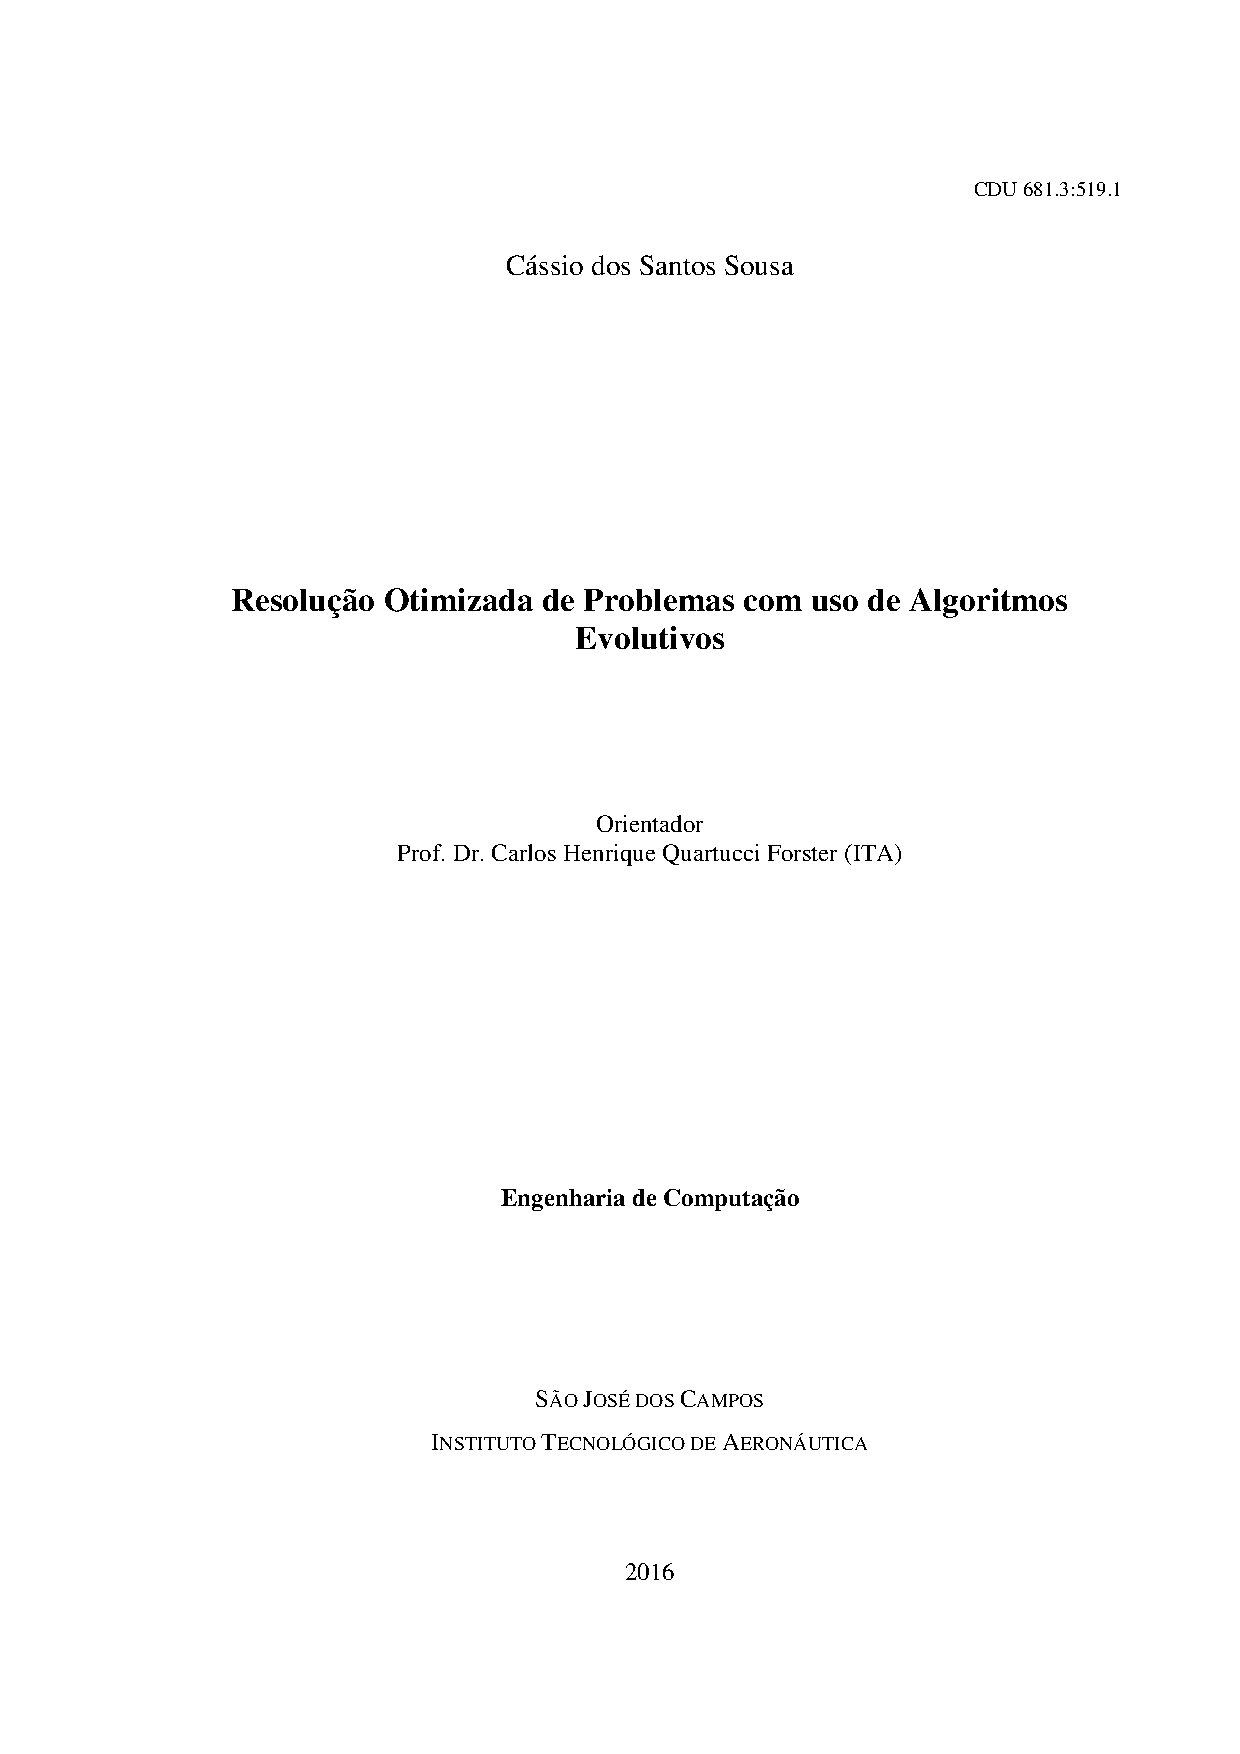
\includepdf{folha_rosto_tg.pdf}
\bookmark[level=0, page=2]{Folha de Rosto}

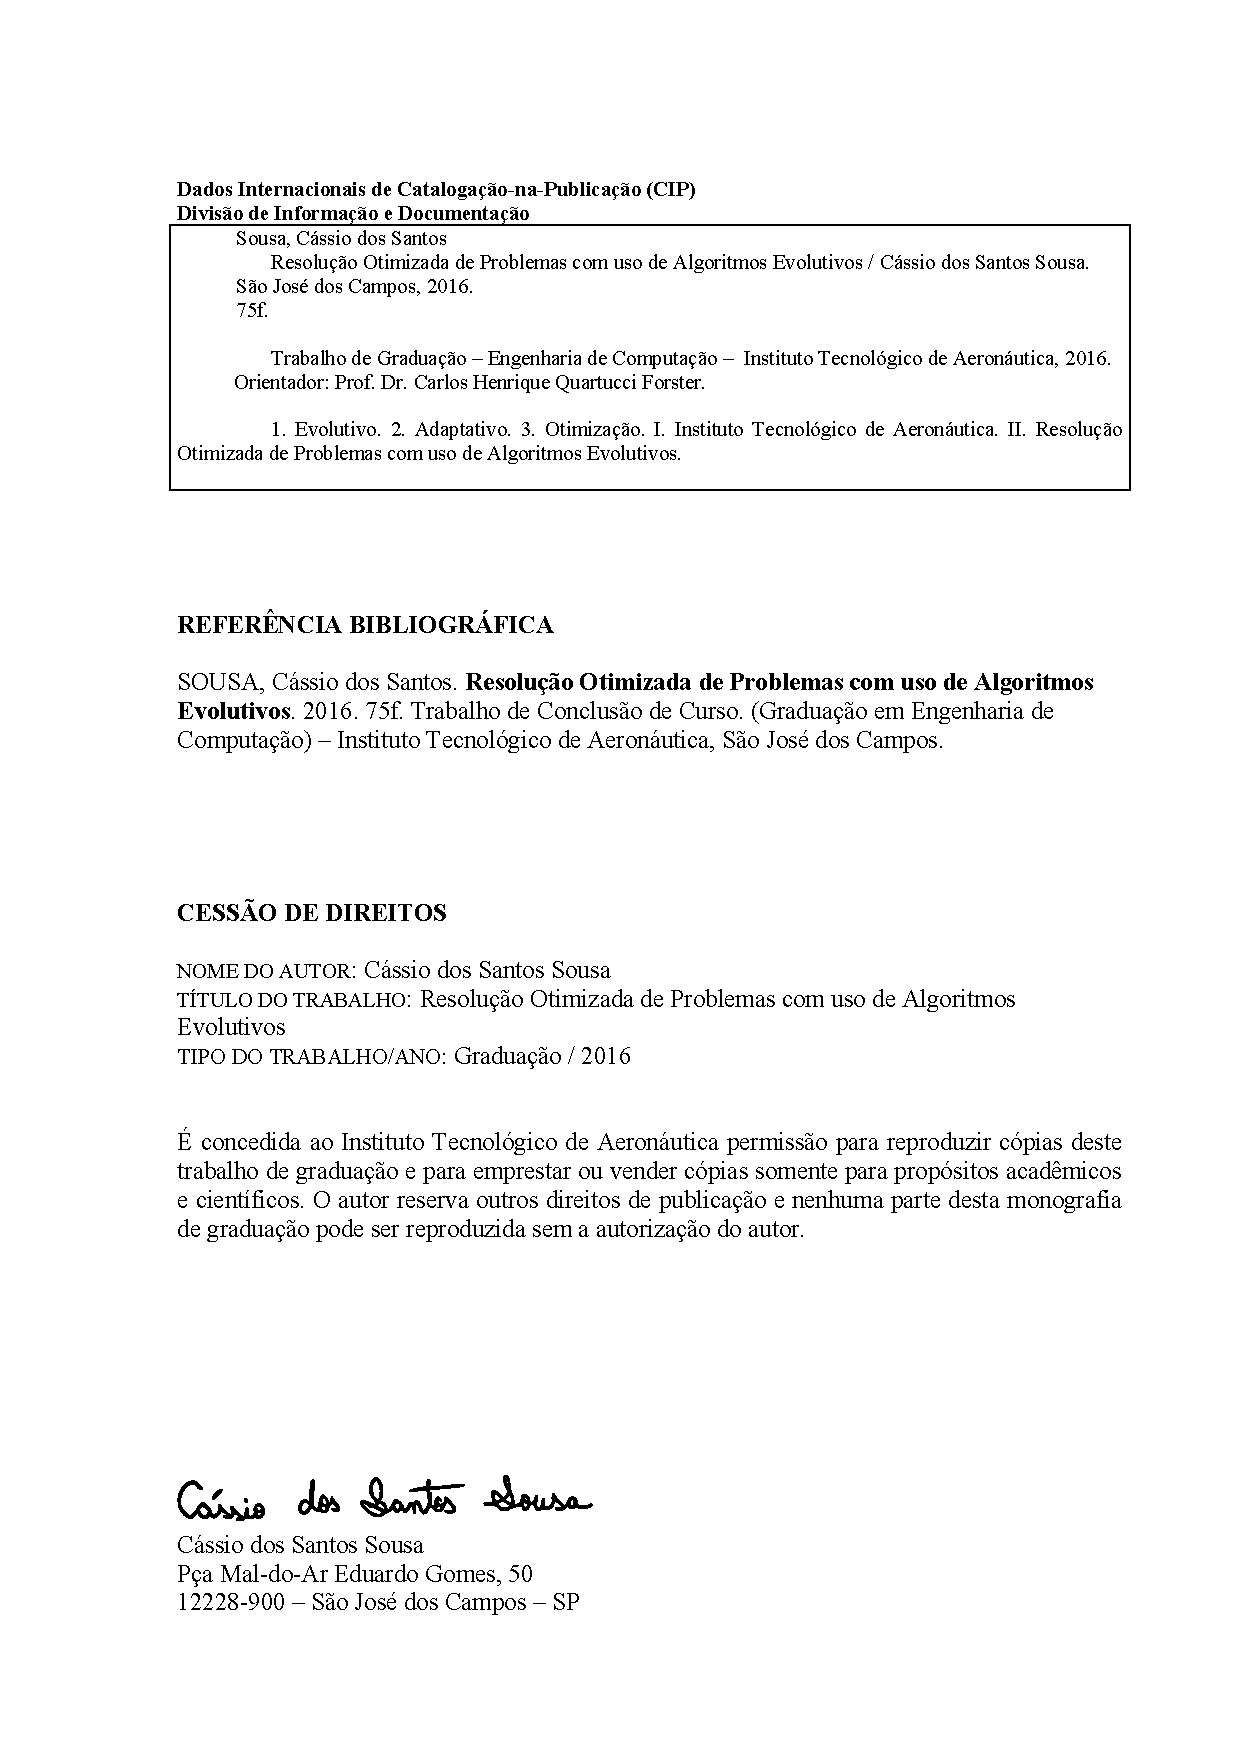
\includepdf{verso_folha_rosto_tg.pdf}
\bookmark[level=0, page=3]{Verso da Folha de Rosto}


\includepdf{folha_aprovacao_tg.pdf}
\bookmark[level=0, page=4]{Folha de Aprova\cao}

\vspace*{18cm}

\begin{flushright}
\begin{minipage}[t]{7.0 cm}
Dedico este trabalho � minha m�e Lucinez, que me trouxe suporte durante todo meu tempo no ITA, e ao Instituto Ismart, oportunidade que muda a minha vida desde 2006.
\end{minipage}
\end{flushright}
\thispagestyle{empty}
\bookmark[level=0, page=5]{Dedicat\'oria}

\chapter*{Agradecimentos}
� minha fam�lia, que se esfor�ou tanto para que eu ficasse at� o fim no ITA.

Ao meu professor orientador Carlos Forster, que me guiou por caminhos tortuosos at� a conclus�o deste trabalho de gradua��o.

Aos meus colegas de turma, que foram uma fam�lia a mais enquanto estive no ITA, e que despertaram em mim o desejo de sempre voar mais alto.

Aos demais professores da COMP, que nos acompanham desde antes do Curso Profissional, e que podem nos ver hoje como verdadeiros engenheiros.

E ao Instituto Ismart, que investe em minha forma��o acad�mica, profissional e pessoal desde 2006 com muito amor e carinho.

\newpage
\thispagestyle{empty}

\vspace*{15.0 cm}

\textit{When you are inspired by some great purpose, some extraordinary project, all your thoughts break their bounds. Your mind transcends limitations, your consciousness expands in every direction and you find yourself in a new, great and wonderful world. Dormant forces, faculties and talents become alive, and you discover yourself to be a greater person by far than you ever dreamed yourself to be.}

\begin{flushright}

Pata�jali, criador das pr�ticas do Ioga.

\end{flushright}
\thispagestyle{empty}
\bookmark[level=0, page=7]{Cita\cao}

\chapter*{Resumo}
A extra��o de caracter�sticas musicais de sinais sonoros � uma tarefa com aplica��o em diversas �reas como compress�o de sinais, ensino, edi��o musical, etc. Todavia, extrair informa��es de um sinal sonoro gravado com instrumentos reais � uma tarefa complexa. Apesar de diversos m�todos j� terem sido desenvolvidos para extra��o de caracter�sticas como tom, intensidade e dura��o de notas, existem poucos trabalhos que unificam essas etapas com alta confiabilidade, o que se reflete na escassez de produtos comerciais capazes de interpretar musicalmente sinais sonoros de forma fiel. Este trabalho objetiva a implementa��o de um programa capaz de realizar em tempo real a transcri��o musical de sinais sonoros, mesmo que ruidosos, para nota��o musical moderna. Para tornar o problema trat�vel, o estudo foi desenvolvido visando a an�lise de sinais provenientes de instrumentos de sopro temperados e monof�nicos, embora tamb�m sejam apresentados resultados obtidos ao analisar outros tipos de instrumento. O programa desenvolvido pode ser dividido em 3 m�dulos principais, respons�veis pela an�lise de tom, intensidade e tempo. A extra��o de tom � feita utilizando uma adapta��o do algoritmo de produto espectral harm�nico (HPS), a de intensidade pelo c�lculo da raiz quadr�tica m�dia e a de tempo por algoritmos de aprendizado. Por fim um m�todo heur�stico utiliza os resultados dos 3 m�dulos para gerar um arquivo MIDI para o sinal, que pode ser facilmente convertido para nota��o musical moderna. O programa desenvolvido foi avaliado utilizando m�sicas do repert�rio cl�ssico ocidental.

\thispagestyle{empty}

\chapter*{Abstract}
This work focused on using Evolutionary Algorithms (EA), more specifically Genetic Algorithms (GA), to solve different problems. Such algorithms work with populations where the smallest portion of an individual is the gene, which contains enough information for the individual to try to solve the problem. The GA developed was used for three problems: Boolean OneMax, with genes expressed by 0 or 1; Real OneMax, with genes expressed in the interval [0, 1); and a variation of the Traveling Salesman Problem, in which it's possible to go through shortcuts between the cities. In order to optimize the GA, two extra implementations were used. The first one was the elitism between generations, keeping the best individual immune to variations. The second one was using not only a static version of the GA, in which the input parameters are fixed during the execution, but also an extra module called Adaptive Genetic Algorithm (AGA), which was added to the GA's code and allows variation parameters (recombination and mutation) to change during the execution. The conclusion of this work was that, since the same GA was used to different problems (with the exception of problem-specific inputs), the treatment that would ease convergence for one problem towards the best solution(s) is not the same for other problems. In terms of optimizations, using an AGA turned out to be effective for finding good solutions. For future works, we suggest, when the focus is to solve a specific problem, to mold the GA to benefit from this choice to the fullest, and use some version of AGA in its implementation, too.

\thispagestyle{empty}

\tableofcontents
\bookmark[level=0, page=10]{Sum\'ario}
\addtocontents{sumario}{\protect\thispagestyle{empty}}
\thispagestyle{empty}
% TODO: Descobrir como tirar numeração do Sumário

\listoffigures
\thispagestyle{empty}
% TODO: Descobrir como tirar numeração da lista de figuras

\listoftables
\thispagestyle{empty}

\listofalgorithms
\thispagestyle{empty}

\lstlistoflistings
\thispagestyle{empty}

\chapter*{Lista de Abreviaturas}
\begin{acronym}
	\acro{AE}{Algoritmo Evolutivo}
	\acro{AG}{Algoritmo Gen\'etico}
	\acro{AGA}{Algoritmo Gen\'etico Adaptativo}
\end{acronym}
\thispagestyle{empty}

\chapter{Introdu\cao}
\label{1_introducao}

A resolução de diversos problemas se dá na forma de algoritmos, de instruções bem definidas. No entanto, alguns algoritmos podem pedir inúmeras instruções até concluírem, o que pode até mesmo inviabilizar a solução encontrada. A Inteligência Artificial pode atuar sobre tais problemas de modo a interagir com o problema e aprender com ele a encontrar uma solução. Ótimos candidatos para esta tarefa são os chamados \emph{Algoritmos Evolutivos (AE)}.

Algoritmos evolutivos são aqueles que se baseiam nos princípios de evolução natural da Biologia, e são aplicados em um modo particular de solução de problemas: o da tentativa-e-erro. Tais algoritmos seguem um framework mais ou menos comum, atuante sobre diferente \emph{gerações} de um problema, por meio de mudanças e combinações de \emph{indivíduos} existentes numa \emph{população} \cite{eiben2003introduction}. Tal framework, conjuntamente com as ações evolutivas, pode ser visto na figura \ref{fig:evolution-framework}.

\begin{figure}[ht!]
    \centering 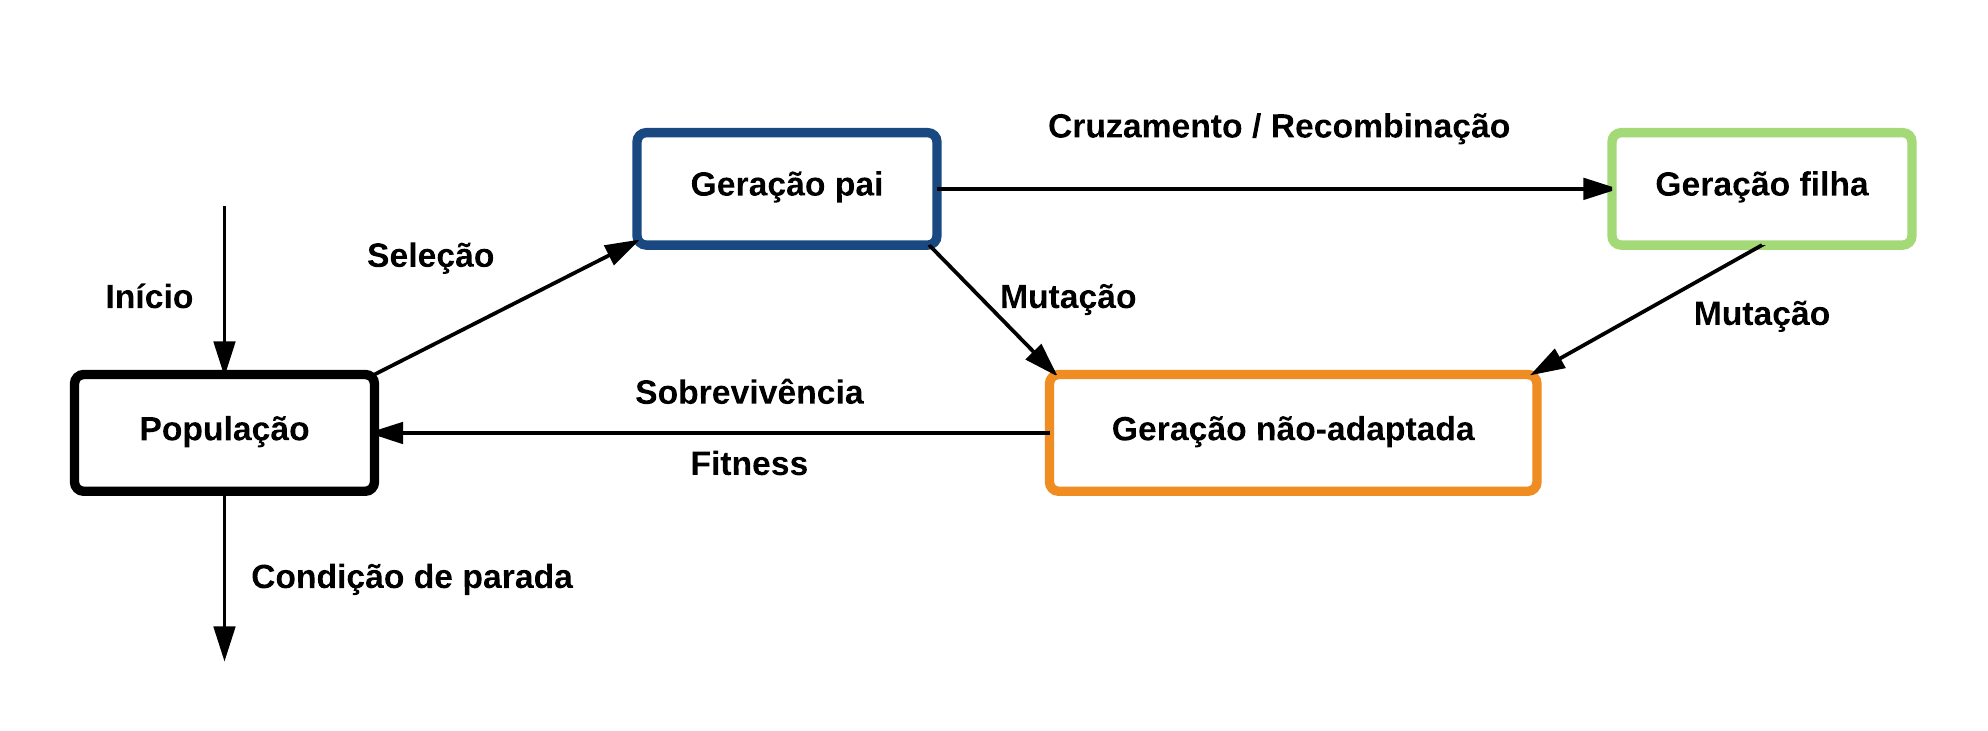
\includegraphics[width=1.0\textwidth]{evolution-framework.png}
    \caption{Framework de um algoritmo evolutivo.}
    \label{fig:evolution-framework}
\end{figure}

Cada indivíduo está tentando resolver o problema durante a execução do algoritmo evolutivo. A população contém estes indivíduos e é o alvo de interesse do processo evolutivo, e uma geração é a população que sobrevive após um ciclo de processos evolutivos do \ac{AE} sobre o problema. Similar ao processo evolutivo, seus componentes principais são as operações de variação (mutação e recombinação) e de seleção (seleção da geração pai e sobrevivência), chamadas aqui simplesmente de \emph{operações de evolução} \cite{eiben2011parameter}.

Este trabalho se utilizou de um grupo específico de Algoritmo Evolutivo, chamado de \textbf{Algoritmo Genético (AG)}. Um AG possui, como a menor estrutura de seus indivíduos, o \emph{gene}. Um gene costuma ter apenas duas propriedades: uma expressividade, normalmente associada a um valor numérico, e uma forma de mudá-la aleatoriamente.

Para um AG, a \emph{mutação} é uma mudança não controlada de um indivíduo feita a partir da mudança na expressividade de um ou mais genes. A \emph{recombinação} envolve a mistura de genes vindos de dois indivíduos que são cruzados. A \emph{seleção} envolve uma escolha a dedo dos melhores exemplares para cruzamento (a geração pai). A \emph{sobrevivência} envolve a rejeição de indivíduos que não estejam aptos o suficiente para resolver o problema. Tal aptidão é normalmente associada a uma função definida conjuntamente com o problema, chamada de \emph{função de fitness}.

\section{Objetivo}

Este trabalho propôs implementar um algoritmo genético capaz de resolver problemas determinados de diferentes complexidades e encontrar boas soluções após uma quantidade razoável de gerações.

\section{Abordagem}

Em termos de implementação, o AG deve ser tal que, uma vez aplicado sobre um problema e uma população, as gerações se desenvolvam automaticamente. O trabalho foi então dividido em 4 etapas:

\begin{enumerate}[label={[\arabic*]}]
	\item Escolha e implementação de problemas compatíveis com a aplicação do AE;
	\item Implementação do AG e de suas operações de evolução;
	\item Otimização do AG;
	\item Análise de performance e coleta de dados.
\end{enumerate}

As primeiras duas etapas são interdependentes, e precisaram ser completadas primeiro e conjuntamente. As demais etapas foram feitas sequencialmente, e foi encima da última etapa que as conclusões foram feitas.

De modo a permitir a reutilização deste código em outros problemas, o AG foi feito de modo a ser compatível com mais de um problema. As ferramentas de análise e coleta de dados consideraram tanto métricas comuns da literatura quanto parâmetros específicos dos problemas abordados.

Optou-se por utilizar Python como linguagem principal do código feito para este trabalho.

\section{Plano de Trabalho}
\label{sec:plano_trabalho}

Este trabalho foi planejado de forma que as etapas de otimização e análise do AE demorassem mais tempo. A validação dos resultados foi feita com base na literatura encontrada e nos resultados obtidos por algoritmos de código aberto (\emph{open source}) aplicados aos mesmos problemas.

\section{Organização do Trabalho}

\begin{itemize}
	\item \textbf{Capítulo 1:} Introdução
	\item \textbf{Capítulo 2:} Problemas Escolhidos
	\item \textbf{Capítulo 3:} Algoritmo Genético
	\item \textbf{Capítulo 4:} Otimização do Algoritmo
	\item \textbf{Capítulo 5:} Análises e Resultados
	\item \textbf{Capítulo 6:} Conclusões e Trabalhos Futuros
\end{itemize}


\chapter{Problemas Escolhidos}
\label{2_problemas}

Por mais que a estrutura básica de um algoritmo evolutivo seja capaz de resolver múltiplos problemas, é importante que ele seja validado por problemas de diferentes naturezas. Para isso, este trabalho focou sua atenção na resolução de três problemas com implementações diferentes para a construção do algoritmo genético.

Como o AG atua diretamente com populações, um problema deve defini-las de antemão, tanto em termos de indivíduo quanto em termos de gene. Conjuntamente, é necessário definir quão apto um indivíduo está frente à solução que ele propõe. Isso é feito por meio da \emph{função de fitness}. Para o número de indivíduos na população (ao menos inicialmente), utilizou-se um valor padrão de 100 indivíduos.

Três problemas foram escolhidos: OneMax Booleano \cite{giguere1998population}, OneMax Real e uma adaptação do problema do Caixeiro Viajante \cite{applegate2011traveling}. Os dois primeiros foram escolhidos em termos não só de sua facilidade de implementação, mas também porque são problemas "fáceis" em termos de encontro de solução ótima (como será detalhado a seguir), o que permite testar hipóteses e heurísticas de modo bem mais simples. O terceiro problema foi escolhido por não só ter uma literatura rica, mas também por ser um problema complexo, cujos resultados podem ser analisados e comparados de modo mais rico.

\section{OneMax Booleano}

Dado um conjunto de 100 bits iniciados em 0, o AG deve ser capaz de tornar todos os bits iguais a 1.

\subsection*{Gene}

Utilizou-se aqui o \emph{BooleanGene}, um gene com expressividade booleana (0 ou 1). Sua operação de mutação consiste numa operação semelhante a jogar cara-e-coroa, trocando o valor expresso para 0 ou 1 aleatoriamente, com igual probabilidade.

\subsection*{Indivíduo}

Cada indivíduo tentará resolver o problema, o que faz com que cada indivíduo tenha 100 genes do tipo BooleanGene.

\subsection*{Função de fitness}

Conta-se o número de genes de um indivíduo que sejam iguais a 1. Quanto maior a contagem, melhor.

\section{OneMax Real}

Dado um conjunto de 100 variáveis reais iniciadas em 0, o AG deve ser capaz de tornar todas elas o mais próximo de 1. Este OneMax possui uma caminhada bem mais lenta que o anterior, pois um gene booleano possui apenas dois estados, o que faz com que as ações de mutação permitam uma evolução muito mais rápida, enquanto um gene real muda sua expressividade num espectro bem maior.

\subsection*{Gene}

Utilizou-se aqui o \emph{RealGene}, um gene com expressividade real entre 0.0 e 1.0. Sua operação de mutação consiste numa escolha aleatória de um número real no intervalo [0.0, 1).

\subsection*{Indivíduo}

Cada indivíduo tentará resolver o problema, o que faz com que cada indivíduo tenha 100 genes do tipo RealGene.

\subsection*{Função de fitness}

Soma-se a expressividade de todos os genes de um indivíduo. Quanto maior a contagem, melhor. Feita de maneira apropriada, esta função pode ser a mesma utilizada para o OneMax Booleano.

\section{Caixeiro Viajante Adaptado}

Dado um conjunto de cidades e as distâncias entre elas, o AG deve ser capaz de descobrir qual o menor caminho que possibilita a um caixeiro visitar todas as cidades e retornar à cidade original. Tal problema é NP-Hard, e avaliar se uma solução candidata é algo tão complexo quanto a resolução do problema em si.

Este problema é uma adaptação do original por não obrigar ao problema que as cidades sejam visitadas uma única vez. Isso permite que um indivíduo possa atravessar duas cidades através de um atalho que passe por outras cidades (com isso, o grafo não precisa ser completo).

\subsection*{Gene}

Utilizou-se o \emph{IntegerGene}, um gene com expressividade inteira entre 0 e K-1, com uma operação de mutação capaz de escolher aleatoriamente um valor inteiro neste intervalo. A inicialização deste gene possui K como parâmetro.

\subsection*{Indivíduo}

No caso de um indivíduo do problema do Caixeiro Viajante, foi pensado que o mesmo deveria ser capaz de gerar, a partir da expressividade de seus genes, um percurso que passasse uma única vez por todas as cidades. Para isso, os genes aqui foram organizados de modo um pouco diferente dos problemas OneMax.

Digamos, por exemplo, que um caixeiro na cidade A precise passar pelas cidades [B, C, D, E, F] e voltar à cidade A. O indivíduo de tal problema teria então quatro genes (o número total de cidades, menos dois) criados da seguinte forma:

\begin{itemize}
	\item O primeiro gene possui expressividade de 0 a 4;
	\item O segundo gene possui expressividade de 0 a 3;
	\item O terceiro gene possui expressividade de 0 a 2;
	\item O quarto gene possui expressividade de 0 a 1.
\end{itemize}

Digamos que um dos indivíduos do AG tenha, pela expressividade de seus genes, os valores [3, 0, 1, 0]. Para se calcular o percurso feito por tal indivíduo, escolhe-se a cidade da lista naquela posição, a qual é removida antes de se escolher a próxima cidade. Ou seja:

\begin{itemize}
	\item Gene 1: [3] mapeia a cidade E na lista [B, C, D, E, F]. Sem ela, a lista se torna [B, C, D, F];
	\item Gene 2: [0] mapeia a cidade B na lista [B, C, D, F]. Sem ela, a lista se torna [C, D, F];
	\item Gene 3: [1] mapeia a cidade D na lista [C, D, F]. Sem ela, a lista se torna [C, F];
	\item Gene 4: [0] mapeia a cidade C na lista [C, F]. Sem ela, a lista se torna [F].
\end{itemize}

Como [F] foi a única cidade que tais genes não escolheram, ela será visitada por último. Com isso, o indivíduo com genes [3, 0, 1, 0] traz o percurso $A \rightarrow E \rightarrow B \rightarrow D \rightarrow C \rightarrow F \rightarrow A$.

O percurso inicial terá sempre genes com expressividade zero. No exemplo fornecido, o caminho inicial (trazido por [0, 0, 0, 0]) de todos os indivíduos seria $A \rightarrow B \rightarrow C \rightarrow D \rightarrow E \rightarrow F \rightarrow A$.

\subsection*{Função de fitness}

A função de fitness aqui calcula a distância percorrida pelo caixeiro no trajeto completo trazido pelo indivíduo, considerando sempre o menor caminho a ser percorrido entre quaisquer duas cidades. Isso é trazido pelo uso do algoritmo de Dijkstra \cite{dijkstra1959note} no grafo constituído pelas cidades. Seu uso será detalhado melhor a seguir, mas quanto menor a distância que um indivíduo encontrar, melhor.

Como parte do problema do Caixeiro Viajante é o de encontrar um trajeto de menor custo, não é dito à função de fitness qual é a menor distância que o grafo possui.

\subsection*{Algoritmo de Dijkstra}

O algoritmo de Dijkstra possui o seguinte pseudocódigo \cite{cormen2001dijkstra}:

\begin{algorithm}[H]
$\textbf{Dijkstra(} Grafo, cidade \textbf{)}$
\Begin{
	$Inicializar(Q)$\;
	$Inicializar(dist)$\;
	$Inicializar(prev)$\;
	\ForEach{cidade v no Grafo} {
		$dist[v] \gets \infty$\;
		$prev[v] \gets desconhecido$\;
		$Q.adicionar(v)$\;
	}
	$dist[cidade] \gets 0$\;
	\While{Q não estiver vazio} {
		$u \gets VerticeEmQComMenorDist(Q, dist)$\;
		$Q.remover(u)$\;
		\ForEach{Vizinho w de u} {
			$atalho \gets dist[u] + DistanciaEntre(u, w)$\;
			\If{atalho < dist[w]} {
				$dist[w] \gets atalho$\;
				$prev[w] \gets u$\;
			}
		}
	}
	\Return{dist, prev}
}
\caption{Pseudocódigo do Algoritmo de Dijkstra.}
\label{alg:dijkstra}
\end{algorithm}

A complexidade de tal algoritmo, por possuir um loop dentro de outro, é, para o pior caso, $O(N^2)$, sendo $N$ o número de cidades. No entanto, ele só descobre a menor distância tendo como referência a cidade utilizada como parâmetro. Por conta disso, o algoritmo precisa ser rodado uma vez para cada cidade, trazendo uma complexidade total $O(N^3)$ para o seu uso.

O requerimento para este algoritmo convergir é o de que a distância entre quaisquer duas cidades seja maior que zero. Para ser utilizada com o AG, foi considerado também que o grafo fosse conexo, de tal forma que qualquer percurso sugerido por um indivíduo tenha uma distância total finita e não-nula.

O algoritmo de Dijkstra tenta buscar atalhos entre quaisquer duas cidades em sua execução. Se ele for utilizado para completar o grafo, um percurso como $A \rightarrow B$ pode pedir que sejam visitadas outras cidades (o que, em casos reais de mapeamento de cidades, é comum acontecer).

Um indivíduo que propuser um percurso não saberá dizer se há atalhos entre duas cidades. No entanto, como estamos procurando a menor distância a ser percorrida no grafo, a função de fitness irá visitar todos os atalhos, sem considerar tal cidade como visitada. Esperou-se que, ao longo das gerações, os atalhos acabassem sendo escolhidos para visita naturalmente.


\chapter{Algoritmo Gen\'etico}
\label{3_algoritmo_genetico}

O pseudocódigo tradicional de um algoritmo evolutivo pode ser dado por \cite{algoritmopseudo}:

\begin{algorithm}[H]
\Begin{
$P \gets InicializarPopulacao(fitness)$\;
$P.fitness()$\;
$t = 0$\;
\While{t < número de gerações} {
	$Pais \gets Selecao(P)$\;
	$Filhos \gets Crossover(Pais)$\;
	$P \gets P \cup Filhos$\;
	$Mutacao(P)$\;
	$P.fitness()$\;
	$P \gets Sobrevivem(P)$\;
}
}
\caption{Pseudocódigo do Algoritmo Genético.}
\label{alg:ag}
\end{algorithm}

Cada uma destas funções principais (todas exceto a função de fitness, que é uma das entradas do problemas) pode ser feita de diferentes maneiras. No entanto, tais implementações independem do problema a ser resolvido, o que torna sua confecção e manutenção bem mais simples.

\section{Seleção}

A escolha dos pais é feita por.

\section{Crossover}

Escolhidos os pais, optou-se neste trabalho por embaralhá-los aleatoriamente numa lista e, escolhendo-os dois a dois, verificar se os dois pais serão cruzados, de acordo com uma probabilidade $p_c$. Se sim, os pais terão seus materiais genéticos misturados por uma ação chamada \emph{crossover}.

Crossover envolve a quebra da sequência de genes de dois indivíduos em um mesma secção, com a subsequente troca de material na região delimitada por esta secção. Este trabalho se utilizou do crossover em dois pontos, o qual divide as sequências em duas partes distintas, ocorrendo troca do material genético entre estas partes. Tal ação é mostrada na figura \ref{fig:evolution-framework}.

\begin{figure}[ht!]
    \centering 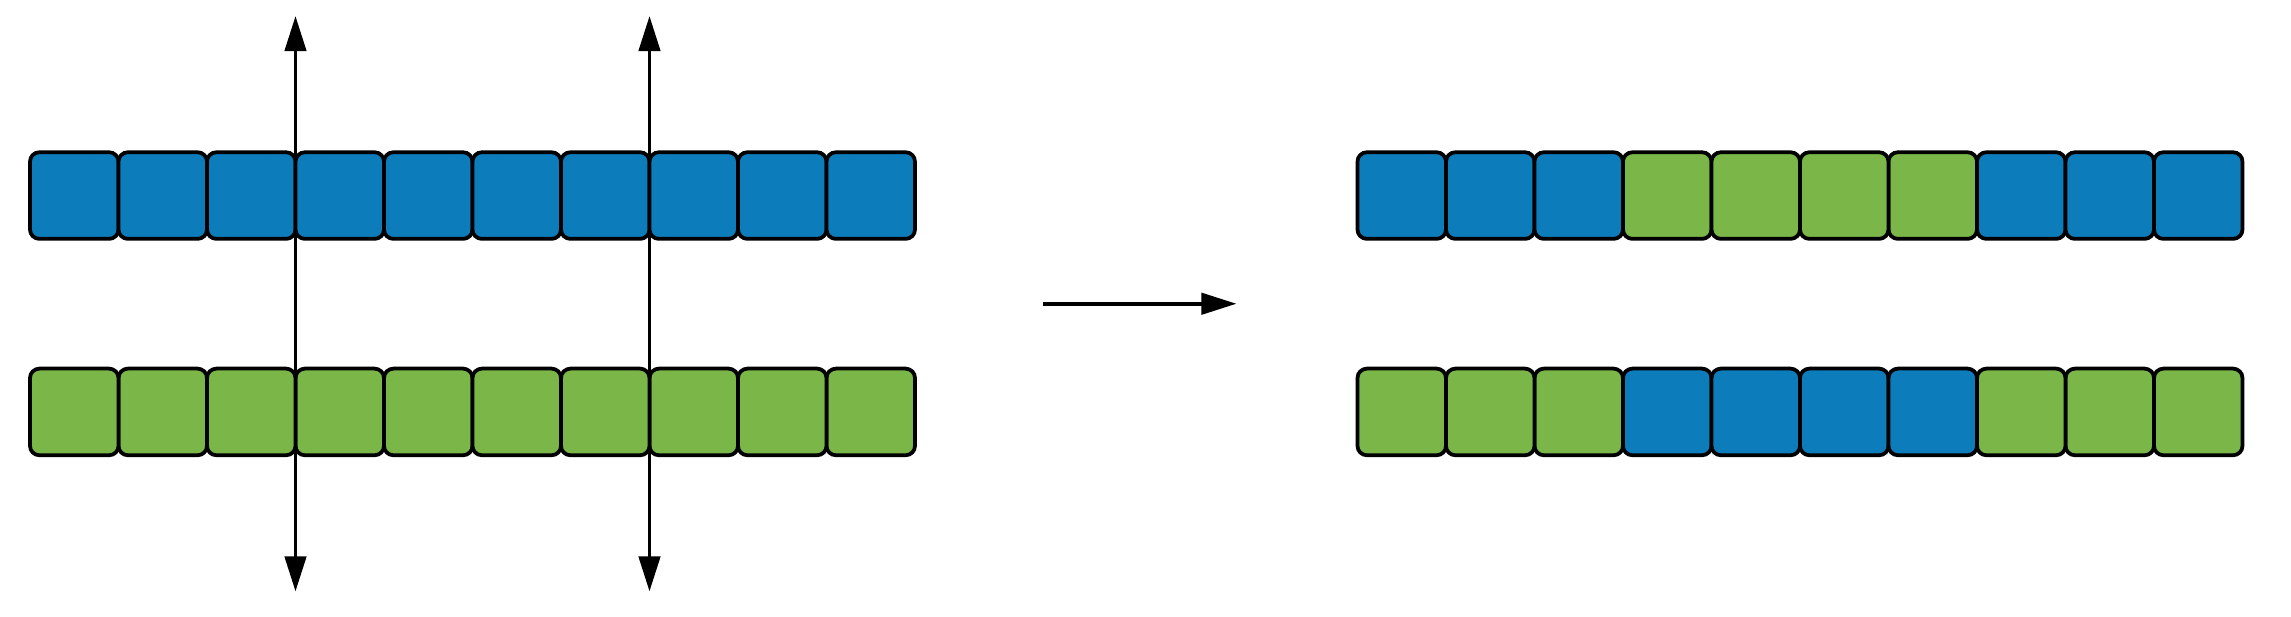
\includegraphics[width=1.0\textwidth]{crossover.png}
    \caption{Ação de crossover em dois pontos.}
    \label{fig:crossover}
\end{figure}

Toda ação de crossover gera duas sequências de genes (filhas) novas a partir das sequências originais (pais), adicionando dois indivíduos novos a cada crossover bem sucedido.

\section{Mutação}

A ação de mutação funciona, em sua estrutura mais básica, da seguinte forma: itera-se sobre todos os genes da população um a um. Com uma probabilidade $p_m$, é avaliado se o gene deveria ou não alterar sua expressividade. Se sim, o gene tem seu valor alterado aleatoriamente.

\section{Sobrevivência}

Texto.



\chapter{Otimização do Algoritmo}
\label{4_otimizacao}

Como proposta deste trabalho, pensou-se em como seria possível otimizar um AG de modo a encontrar boas soluções em poucas gerações. Dado o pseudocódigo de um AE, é possível propor uma série de otimizações, desde aquelas voltadas à melhoria de processamento, como o processamento paralelo de indivíduos em uma dada geração, àquelas que otimizam cada uma das quatro operações evolutivas principais (seleção, recombinação, mutação e sobrevivência).

De modo geral, o que traz novas soluções ao problema são as operações de variação (recombinação e mutação), e por conta disso, foram as mais analisadas neste capítulo. Otimizações mais simples discutidas em outros trabalhos, mas que se mostraram eficazes no encontro ou manutenção de boas soluções, também foram discutidas neste capítulo.

A manutenção de boas soluções foi obtida pelo uso de \emph{elitismo}. A otimização nas operações de variação foi obtida pelo uso dos chamados Algoritmos Genéticos Adaptativos (AGA).

\section{Elitismo}

O elitismo é a manutenção do indivíduo mais adaptado de uma geração, deixando-o imune a mutações para que a melhor solução não seja perdida \cite{mitchell1998introduction}. Um indivíduo elitista ainda pode ser considerado para recombinação e geração de filhos, uma vez que as operações de mutação e recombinação são independentes. É possível também criar um grupo elitista, mantendo-se uma certa quantidade ou porcentagem de indivíduos imune a mutações.

Este trabalho utilizou elitismo para o melhor indivíduo em todas as execuções do AG. Tal propriedade pode ser desativada no código.

\section{Algoritmo Genético Adaptativo (AGA)}

A forma mais tradicional de implementação de um AG atribui valores estáticos aos parâmetros de entrada, incluindo os parâmetros de crossover e mutação. No entanto, os indivíduos buscarão soluções de acordo com estes dois parâmetros, e deixá-los estáticos pode limitar o alcance do AG e impedi-lo de encontrar soluções melhores.

Se fosse possível modificar tais parâmetros enquanto o AG é executado, de modo a se adaptar às mudanças de fitness dos próprios indivíduos, teríamos uma solução. Um bom candidato para isso são os chamados Algoritmos Genéticos Adaptivos (AGAs) \cite{srinivas1994adaptive}.

O conceito por trás de um AGA envolve implementar em cima de um AG de modo a modificar os parâmetros de crossover e/ou mutação ao longo do tempo. Não obstante, é possível moldar um AGA de modo a tratar crossover e mutação com probabilidades diferentes para cada indivíduo, de acordo com seus valores de fitness.

Para este trabalho, optou-se por trabalhar com versões adaptadas de outros AGAs \cite{jakobovic1999adaptive, wang2001improved, srinivas1994adaptive} e implementar uma versão própria, explicada a seguir:

\begin{itemize}

	\item Apenas o parâmetro de mutação é modificado ao longo das gerações, uma vez que o crossover seja sempre um valor alto (como 0.9, padronizado neste trabalho);

	\item A adaptação de $p_m$ acontece apenas depois que um ciclo de operações de evolução acontecer;

	\item O que decidirá se $p_m$ mudará será o desvio do melhor valor de fitness $f_{best}$ em comparação com o fitness médio $\bar{f}$, como na equação a seguir:

\begin{equation}
	\left| \frac{f_{best} - \bar{f}}{\bar{f}} \right|
\label{eq:aga}
\end{equation}

	\item Se este desvio for menor que um valor $p{p_m}_0$, isso significa que a mutação está fraca e os indivíduos estão se aproximando de uma mesma solução, que pode não ser necessariamente a melhor. Para contornar isso, $p_m$ irá aumentar;

	\item Caso contrário, as soluções estarão se desviando muito, o que pode ser resultado de uma mutação intensa. Para resolver isso, $p_m$ irá diminuir;

	\item O valor de ${p_m}_0$ é o valor inicial de $p_m$ para o valor inicial de ${p_m}_0$, de modo a servir de termômetro para o valor do desvio;

	\item No entanto, $p_m$ não pode ser igual a zero nem maior que 1, dado que representa uma probabilidade. Seguindo a linha de outros trabalhos \cite{matthias2013variable}, $p_m$ será limitado ao intervalo [0.001, 0.5] (se $p_m$ tentar extrapolar estes limites, ele retornará ao valor extremo mais próximo);

	\item O incremento/decremento para $p_m$ será linear e igual a 0.001;

	\item Como há uma divisão por $\bar{f}$, se este valor for zero ou muito próximo de zero para alguma geração, este AGA não será executado.

\end{itemize}

Traduzindo-se a explicação para um algoritmo, chegamos ao código mostrado no algoritmo \ref{alg:aga}. Este trabalho avaliará o desempenho deste AGA comparando a evolução da população com e sem o uso do AGA para um mesmo valor inicial de $p_m$. O intuito não foi o de encontrar um AGA ideal, mas sim o de avaliar se o uso dele ajudaria ou não no encontro de soluções melhores.

\begin{algorithm}[ht]
\Begin{
	${p_m}_0 \gets $ (valor inicial de $p_m$ na inicialização do AG)\;
	$\epsilon \gets 0.0001$\;
	\ForEach{ciclo de operações de evolução} {
		$\bar{f} \gets $ (média dos valores de fitness)\;
		\If{$\bar{f} < \epsilon$} {
			\Return
		}
		$f_{best} \gets $ (melhor valor de fitness na população)\;
		$desvio \gets \left| \frac{f_{best} - \bar{f}}{\bar{f}} \right|$\;
		\If{desvio <= ${p_m}_0$} {
			$p_m \gets min(0.5, p_m + 0.001)$\;
		}
		\Else{
			$p_m \gets max(0.001, p_m - 0.001)$\;
		}
	}
}
\caption{Pseudocódigo do Algoritmo Genético Adaptativo (AGA).}
\label{alg:aga}
\end{algorithm}

Para exemplificar o funcionamento do AGA, foram feitas simulações para diferentes valores de ${p_m}_0$ para o OneMax Booleano, na figura \ref{fig:aga_test}. É possível ver que $p_m$ tenta sempre manter o desvio entorno de ${p_m}_0$, incentivando a busca de soluções diferentes para o sistema.

\begin{figure}[ht!]
    \centering 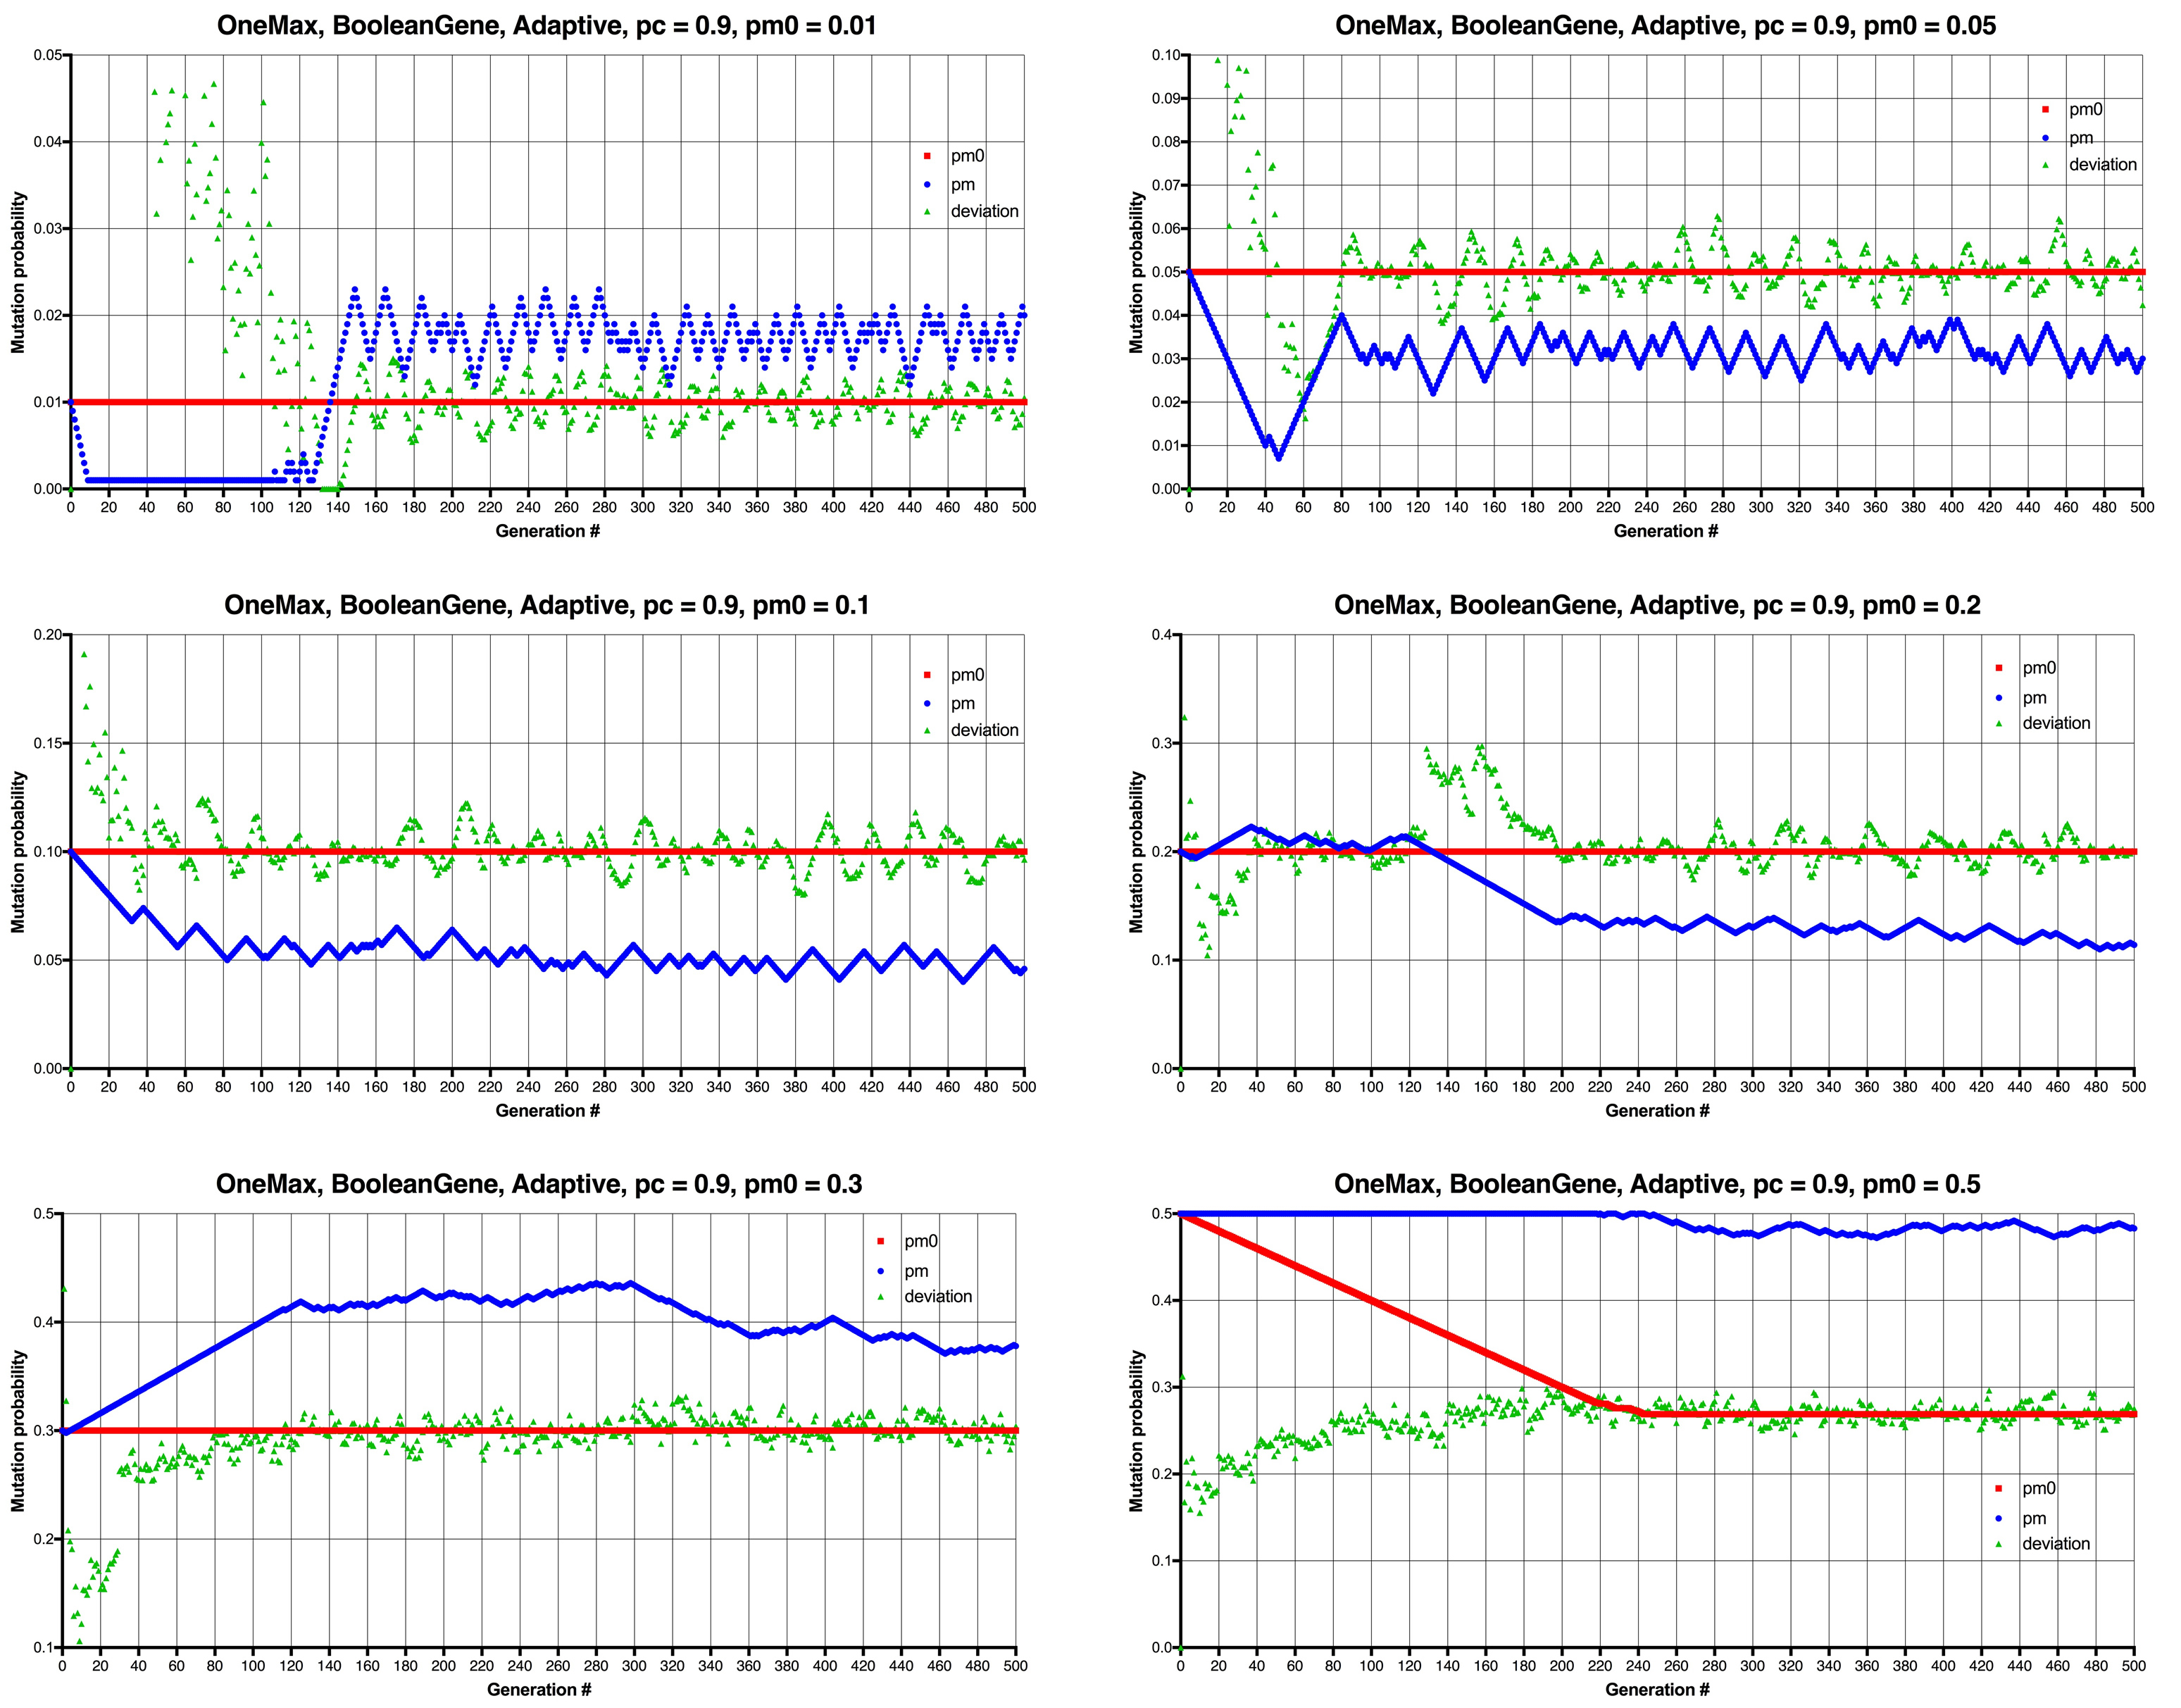
\includegraphics[width=1.0\textwidth]{boolean_onemax_aga.jpg}
    \caption{Evolução dos valores de $p_m$ e ${p_m}_0$ para o problema OneMax para valores diferentes de ${p_m}_0$ (em vermelho) ao longo de 500 gerações. Observa-se que o desvio (em verde) tenta sempre se igualar a ${p_m}_0$, e $p_m$ (em azul) varia de modo a permitir isso.}
    \label{fig:aga_test}
\end{figure}

A ideia por trás de uma implementação própria foi a de testar a implementação de um AGA a partir de conceitos mais simples. Se a ideia de adaptação de um AGA, conforme vista na literatura, for tão simples quanto a base evolutiva do AG, sua implementação também deve buscar algo simples.



\chapter{An\'alises e Resultados}
\label{5_resultados}

\section{Parâmetros analisados}

Como um AG trabalha com tentativa-e-erro, não há uma geração exata para a qual pode ser prevista uma determinada solução (ou proximidade à solução). Para se analisar a evolução dos indivíduos ao longo das gerações, este trabalho focou em analisar os seguintes parâmetros:

\begin{itemize}
	\item Valor mínimo de fitness em um indivíduo;
	\item Valor máximo de fitness em um indivíduo;
	\item Valor médio de fitness entre todos os indivíduos;
	\item Desvio padrão dos valores de fitness.
\end{itemize}

O desvio padrão utilizado aqui foi o amostral, dado por:

\begin{equation}
	\sigma = \sqrt{\frac{1}{N-1} \sum_{i=1}^N (x_i - \overline{x})^2}
\end{equation}

Os gráficos criados tiveram como base uma única simulação do AG para o problema e parâmetros de entrada escolhidos. Não é possível ter expectativas de valores ou gerações, uma vez que o AG trabalha com tentativa-e-erro, então criá-las ou assumi-las seria difícil de quantizar.

Como já foi comentado antes, se não for mencionado o contrário (mesmo para o caso adaptativo), utilizou-se 0.9 para $p_c$ e 0.01 para $p_m$. Todas as execuções utilizaram 100 indivíduos, 200 gerações e elitismo do melhor indivíduo. Se um problema convergiu completamente para a melhor solução antes das 200 gerações completarem, os gráficos foram reduzidos para melhor visualização, uma vez que os pontos extras não trariam novas informações para nós.

As simulações feitas com uso do AGA foram utilizadas para comparação com a implementação estática do AG. Além disso, foi avaliado o comportamento adaptativo de $p_m$ ao longo das gerações.

\section{OneMax Booleano}

\subsection{Caso Estático}

Este problema foi considerado simples de ser resolvido por um AG, uma vez que poucas mutações em um gene já permitem que ele ficasse igual a 1. A figura \ref{fig:onemax_boolean} demonstra exatamente isso, com convergência completa dos indivíduos para a solução ótima após 93 gerações, sendo que a própria solução ótima foi encontrada com a melhor solução aparecendo após 78 gerações.

\begin{figure}[ht!]
    \centering 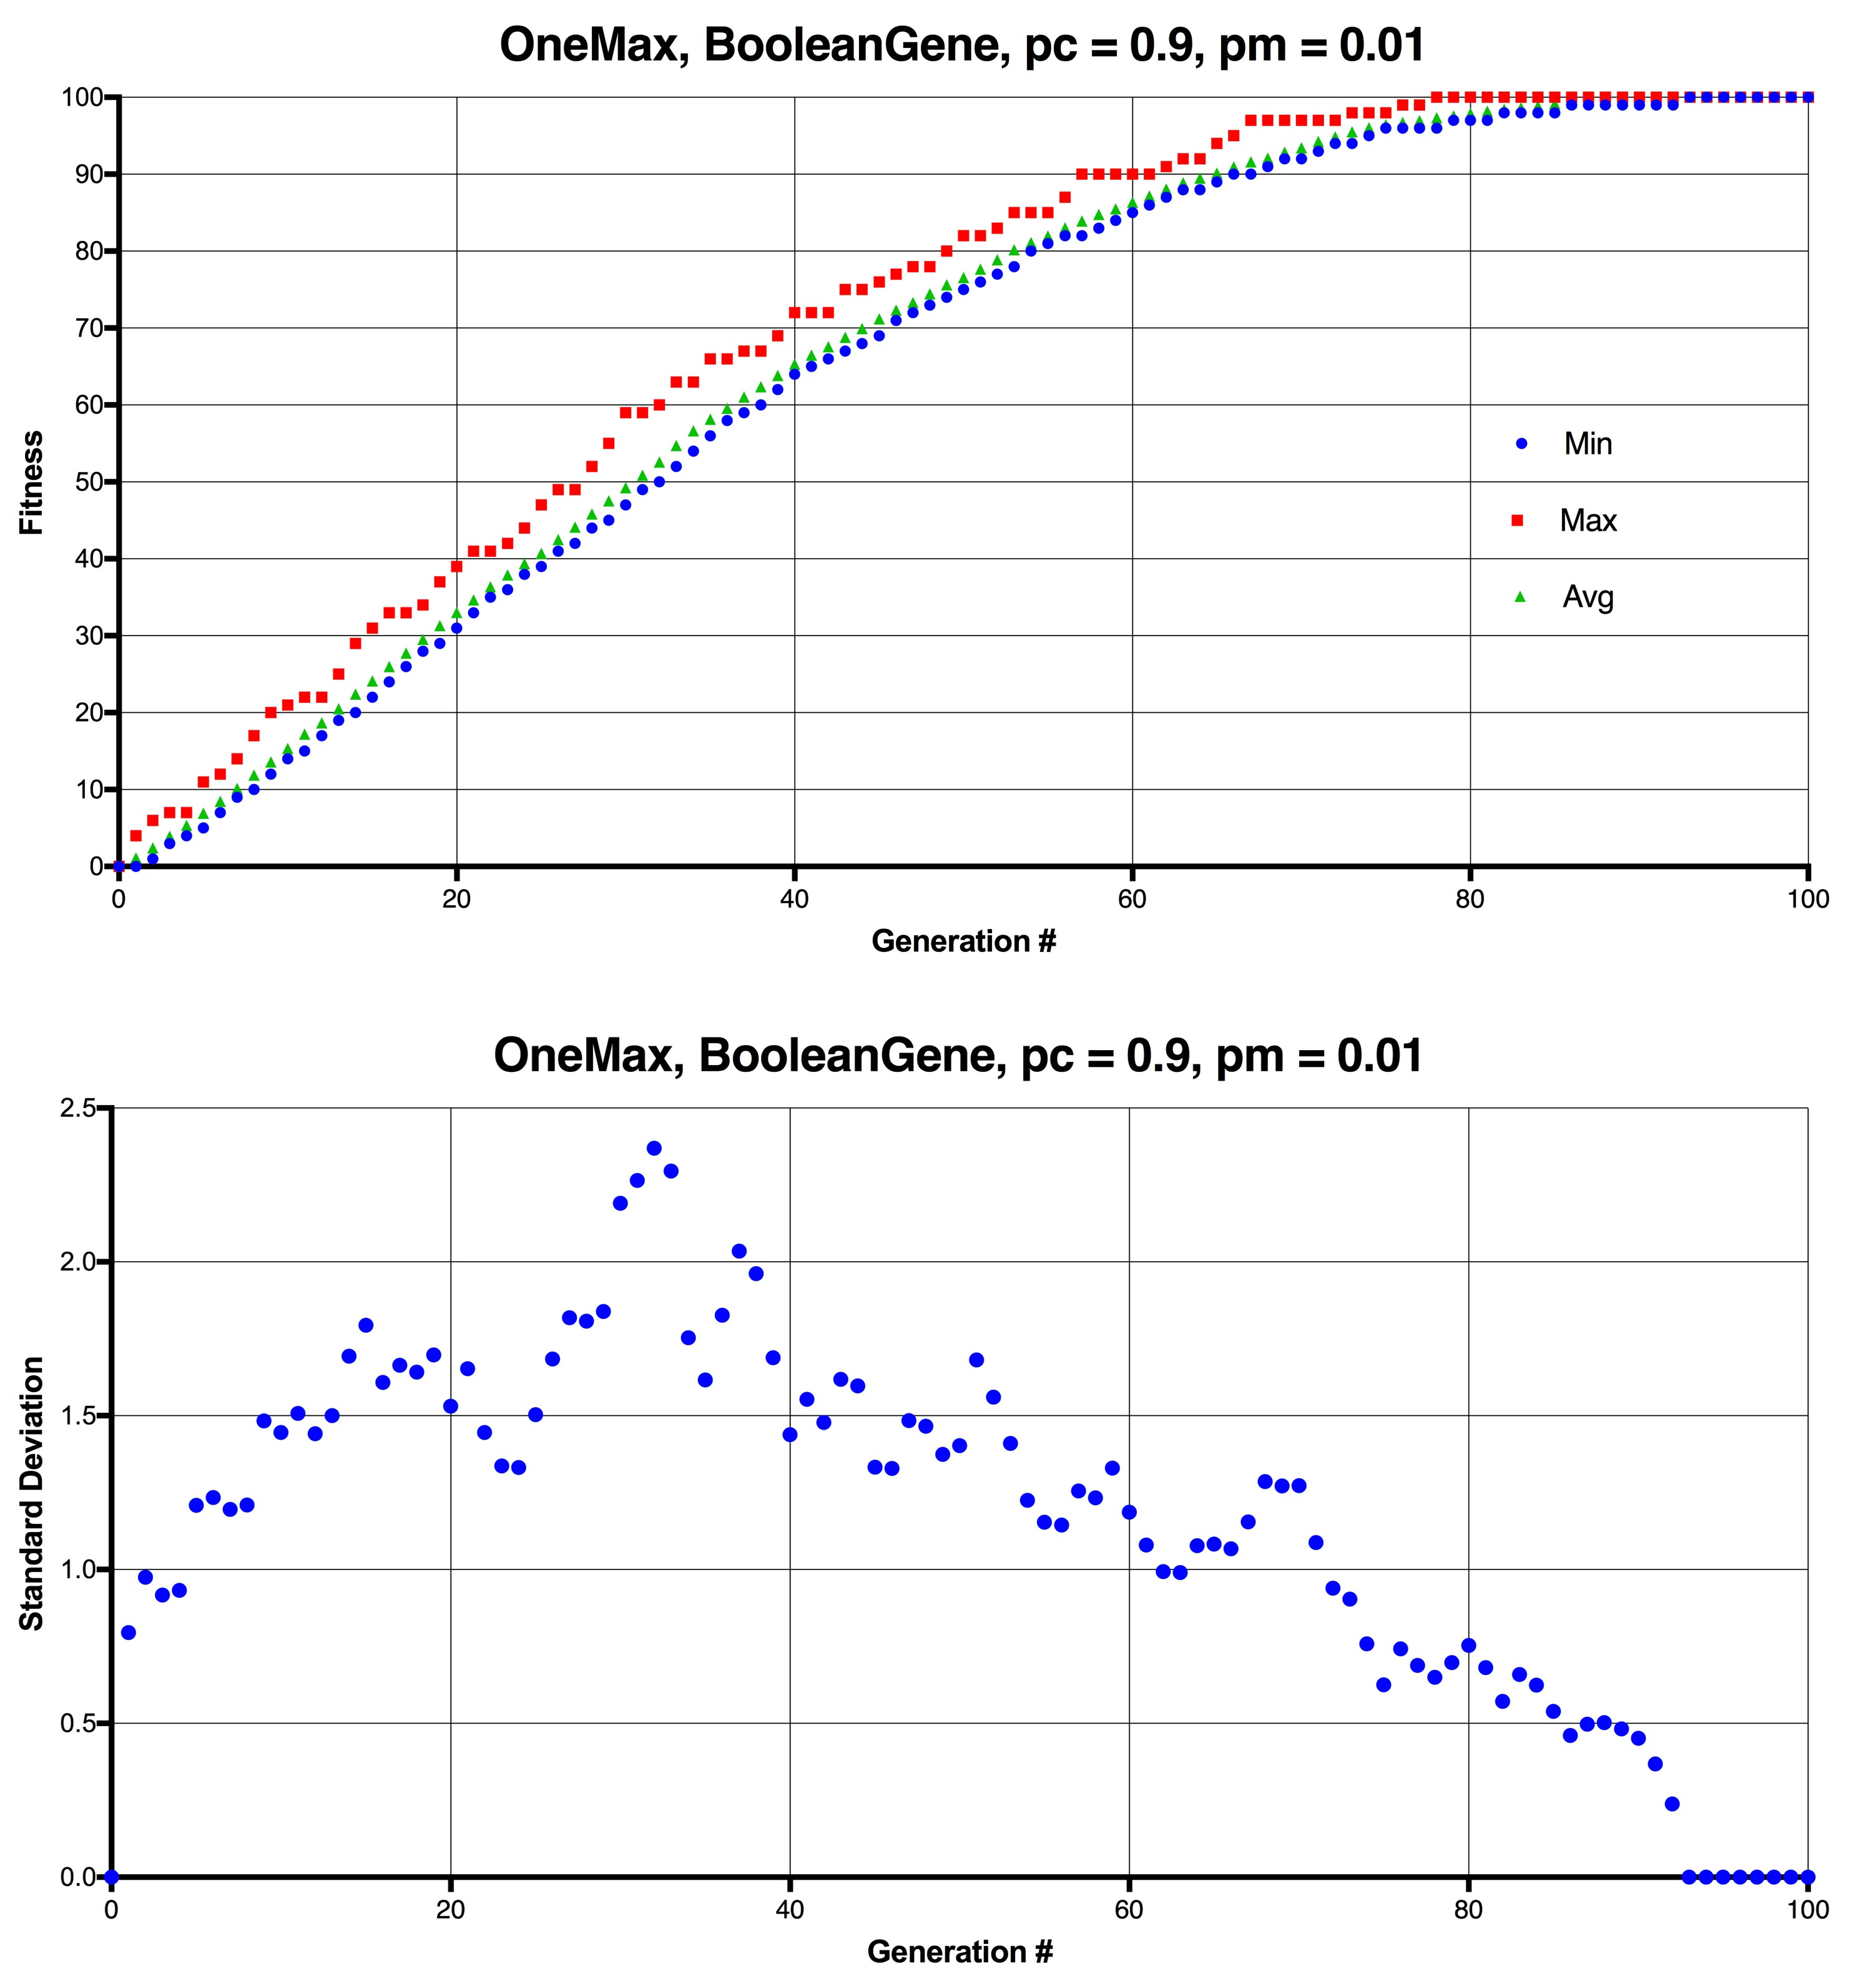
\includegraphics[width=1.0\textwidth]{onemax_boolean.jpg}
    \caption{Evolução do fitness para o problema do OneMax Booleano mostrando mínimo, máximo, valor médio e desvio padrão ($p_c=0.9$, $p_m=0.01$). Foram necessárias 78 gerações para que a solução ótima aparecesse, e 93 gerações para que a população inteira convergisse para ela.}
    \label{fig:onemax_boolean}
\end{figure}

O comportamento estático para os valores padronizados de $p_c$ e $p_m$ mostrou um crescimento aproximadamente linear dos valores de fitness, tanto para o pior quanto para o melhor indivíduo. Isso demonstra que tais valores demonstram um crescimento equilibrado da população, e a mutação existente é suficiente para evoluir os indivíduos.

\subsection{Caso Adaptativo}

Com o AGA ativado, ficou bem mais complicado para o OneMax atingir a solução ótima. Como mostrado na figura \ref{fig:onemax_boolean_adaptive}, foram necessárias 140 gerações para que o melhor indivíduo atingisse a solução ótima, e a média dos valores de fitness oscilou entre 98 e 99 para as últimas gerações. Em termos de desvio padrão, o valor nunca passou de 2.0 (de um máximo de 100), o que nos diz que a população não se dispersou completamente pelo efeito adaptativo.

\begin{figure}[ht!]
    \centering 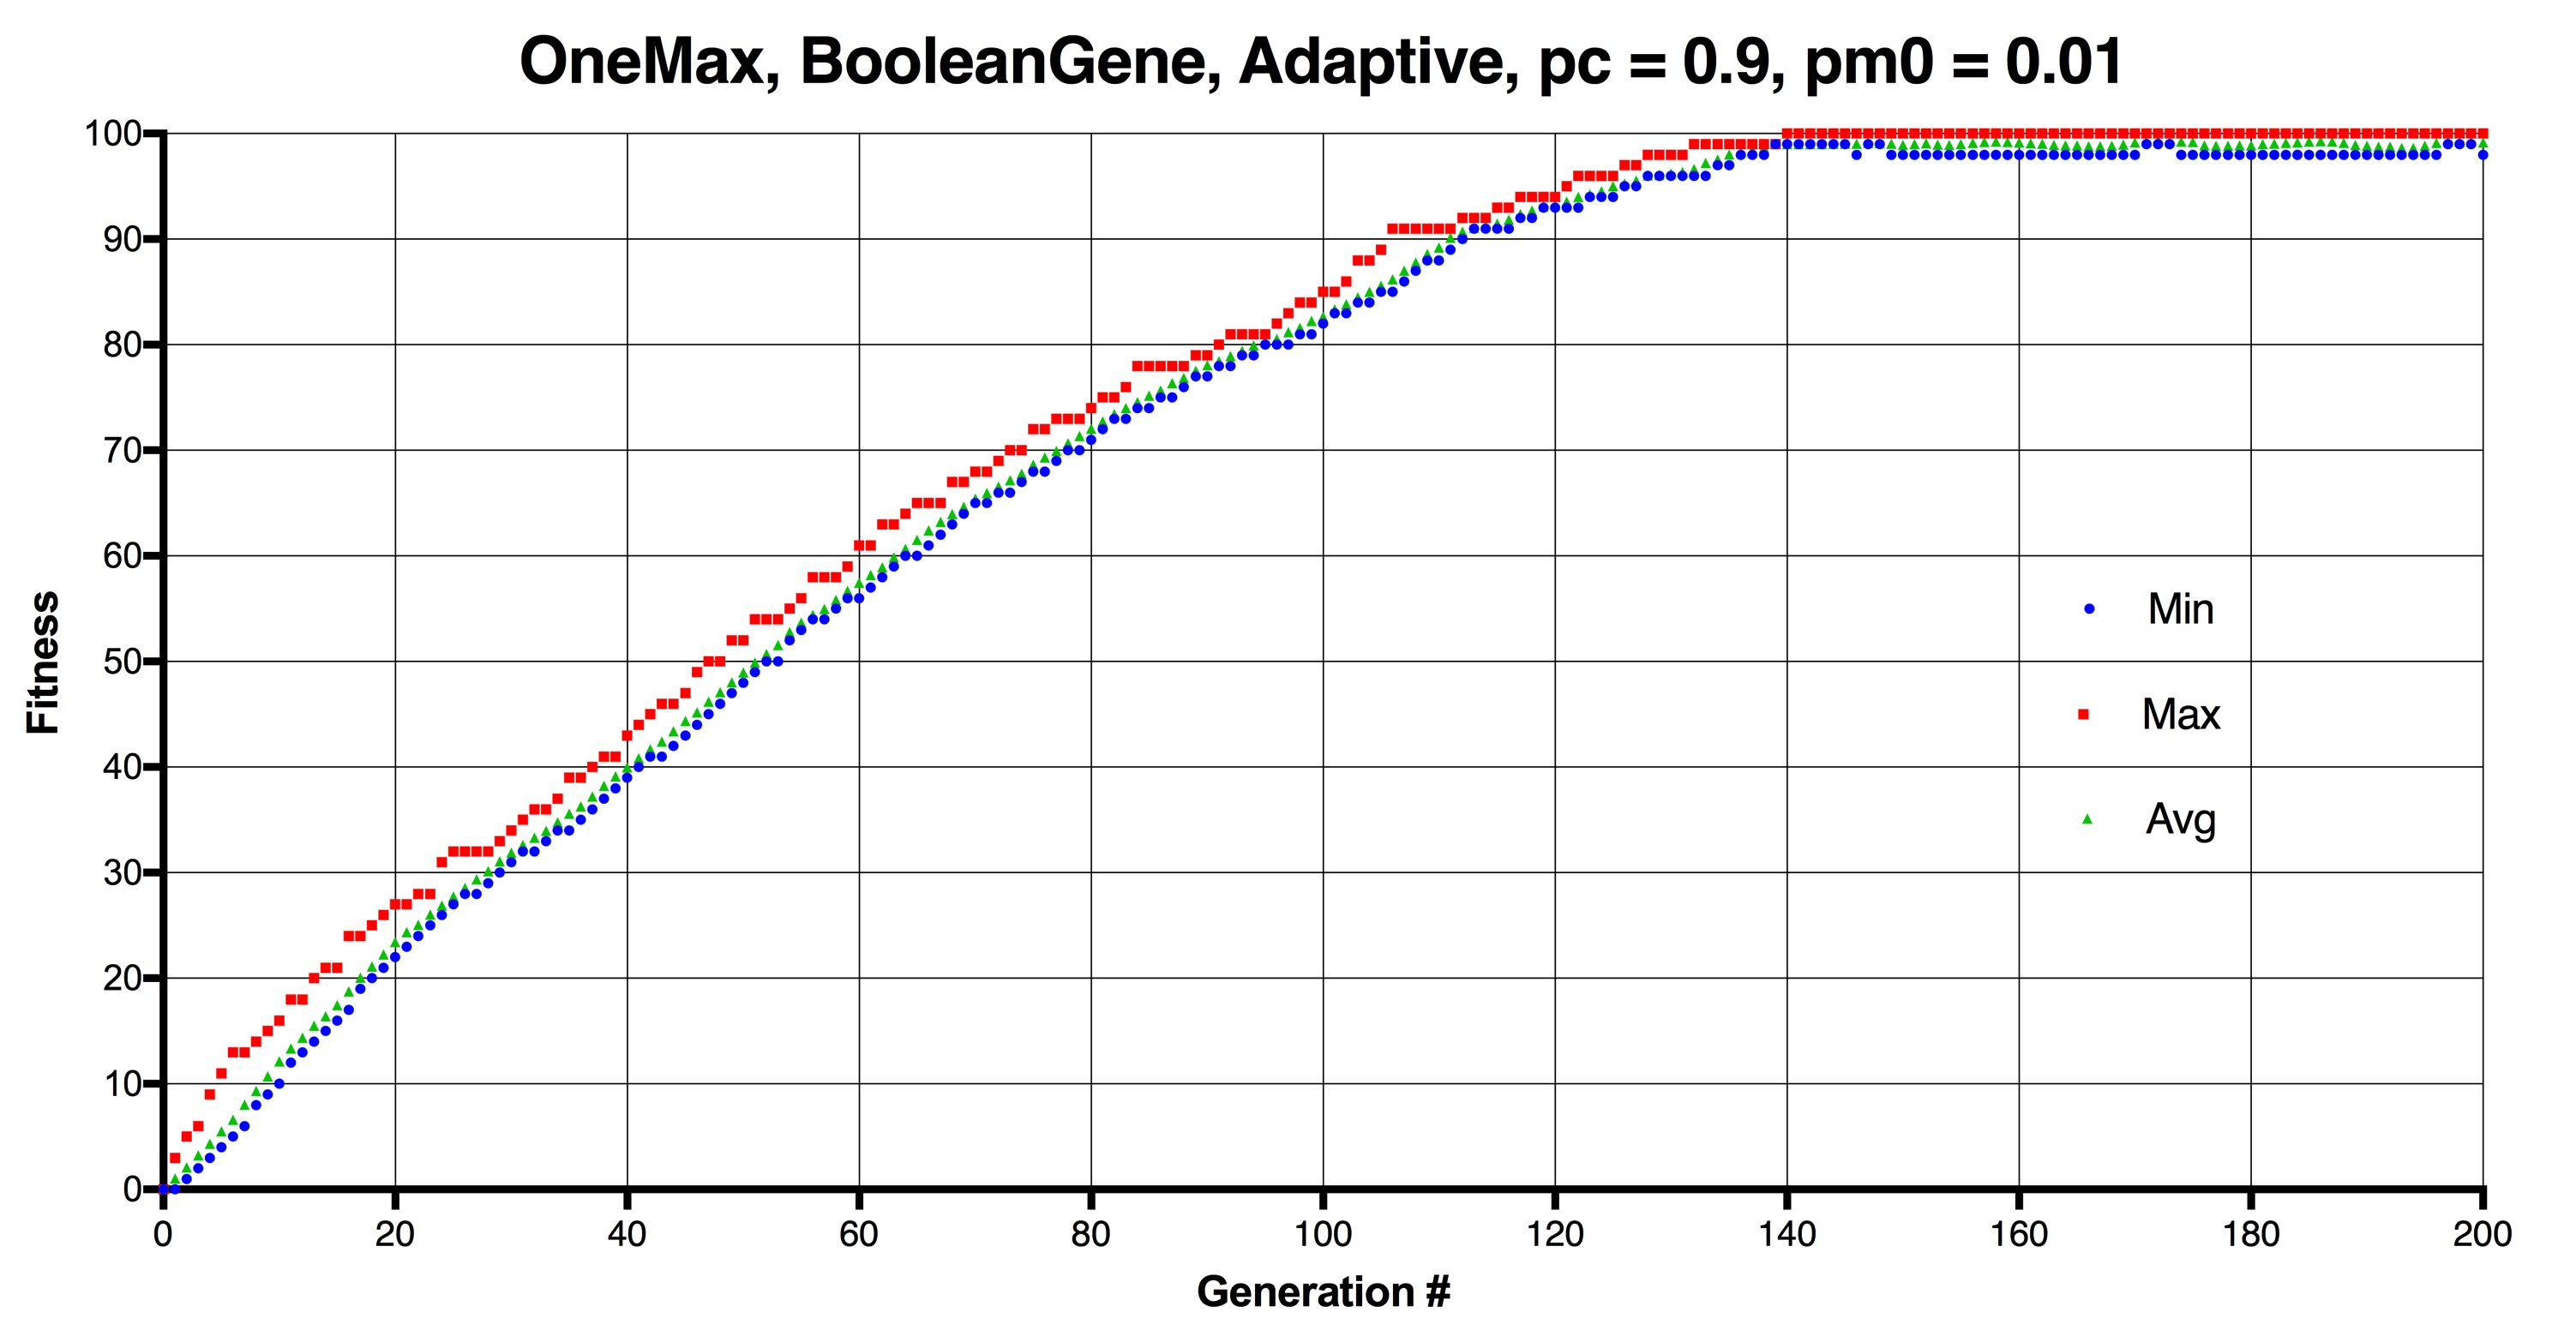
\includegraphics[width=1.0\textwidth]{onemax_boolean_adaptive.jpg}
    \caption{Evolução do fitness para o problema do OneMax Booleano Adaptativo mostrando mínimo, máximo, valor médio e desvio padrão ($p_c=0.9$, ${p_m}_0=0.01$). Foram necessárias 140 gerações para que um indivíduo encontrasse a solução ótima.}
    \label{fig:onemax_boolean_adaptive}
\end{figure}

Um efeito interessante pode ser visto na figura \ref{fig:onemax_boolean_adaptive_pm} com relação à evolução de $p_m$ e ${p_m}_0$. É possível ver que as primeiras gerações ainda eram muito dispersas, o que fez com que $p_m$ começasse a cair. No entanto, como mencionado antes, um valor baixo de $p_m$ se mostrou mais do que suficiente para que a população do caso estático fosse capaz de encontrar a solução ótima.

\begin{figure}[ht!]
    \centering 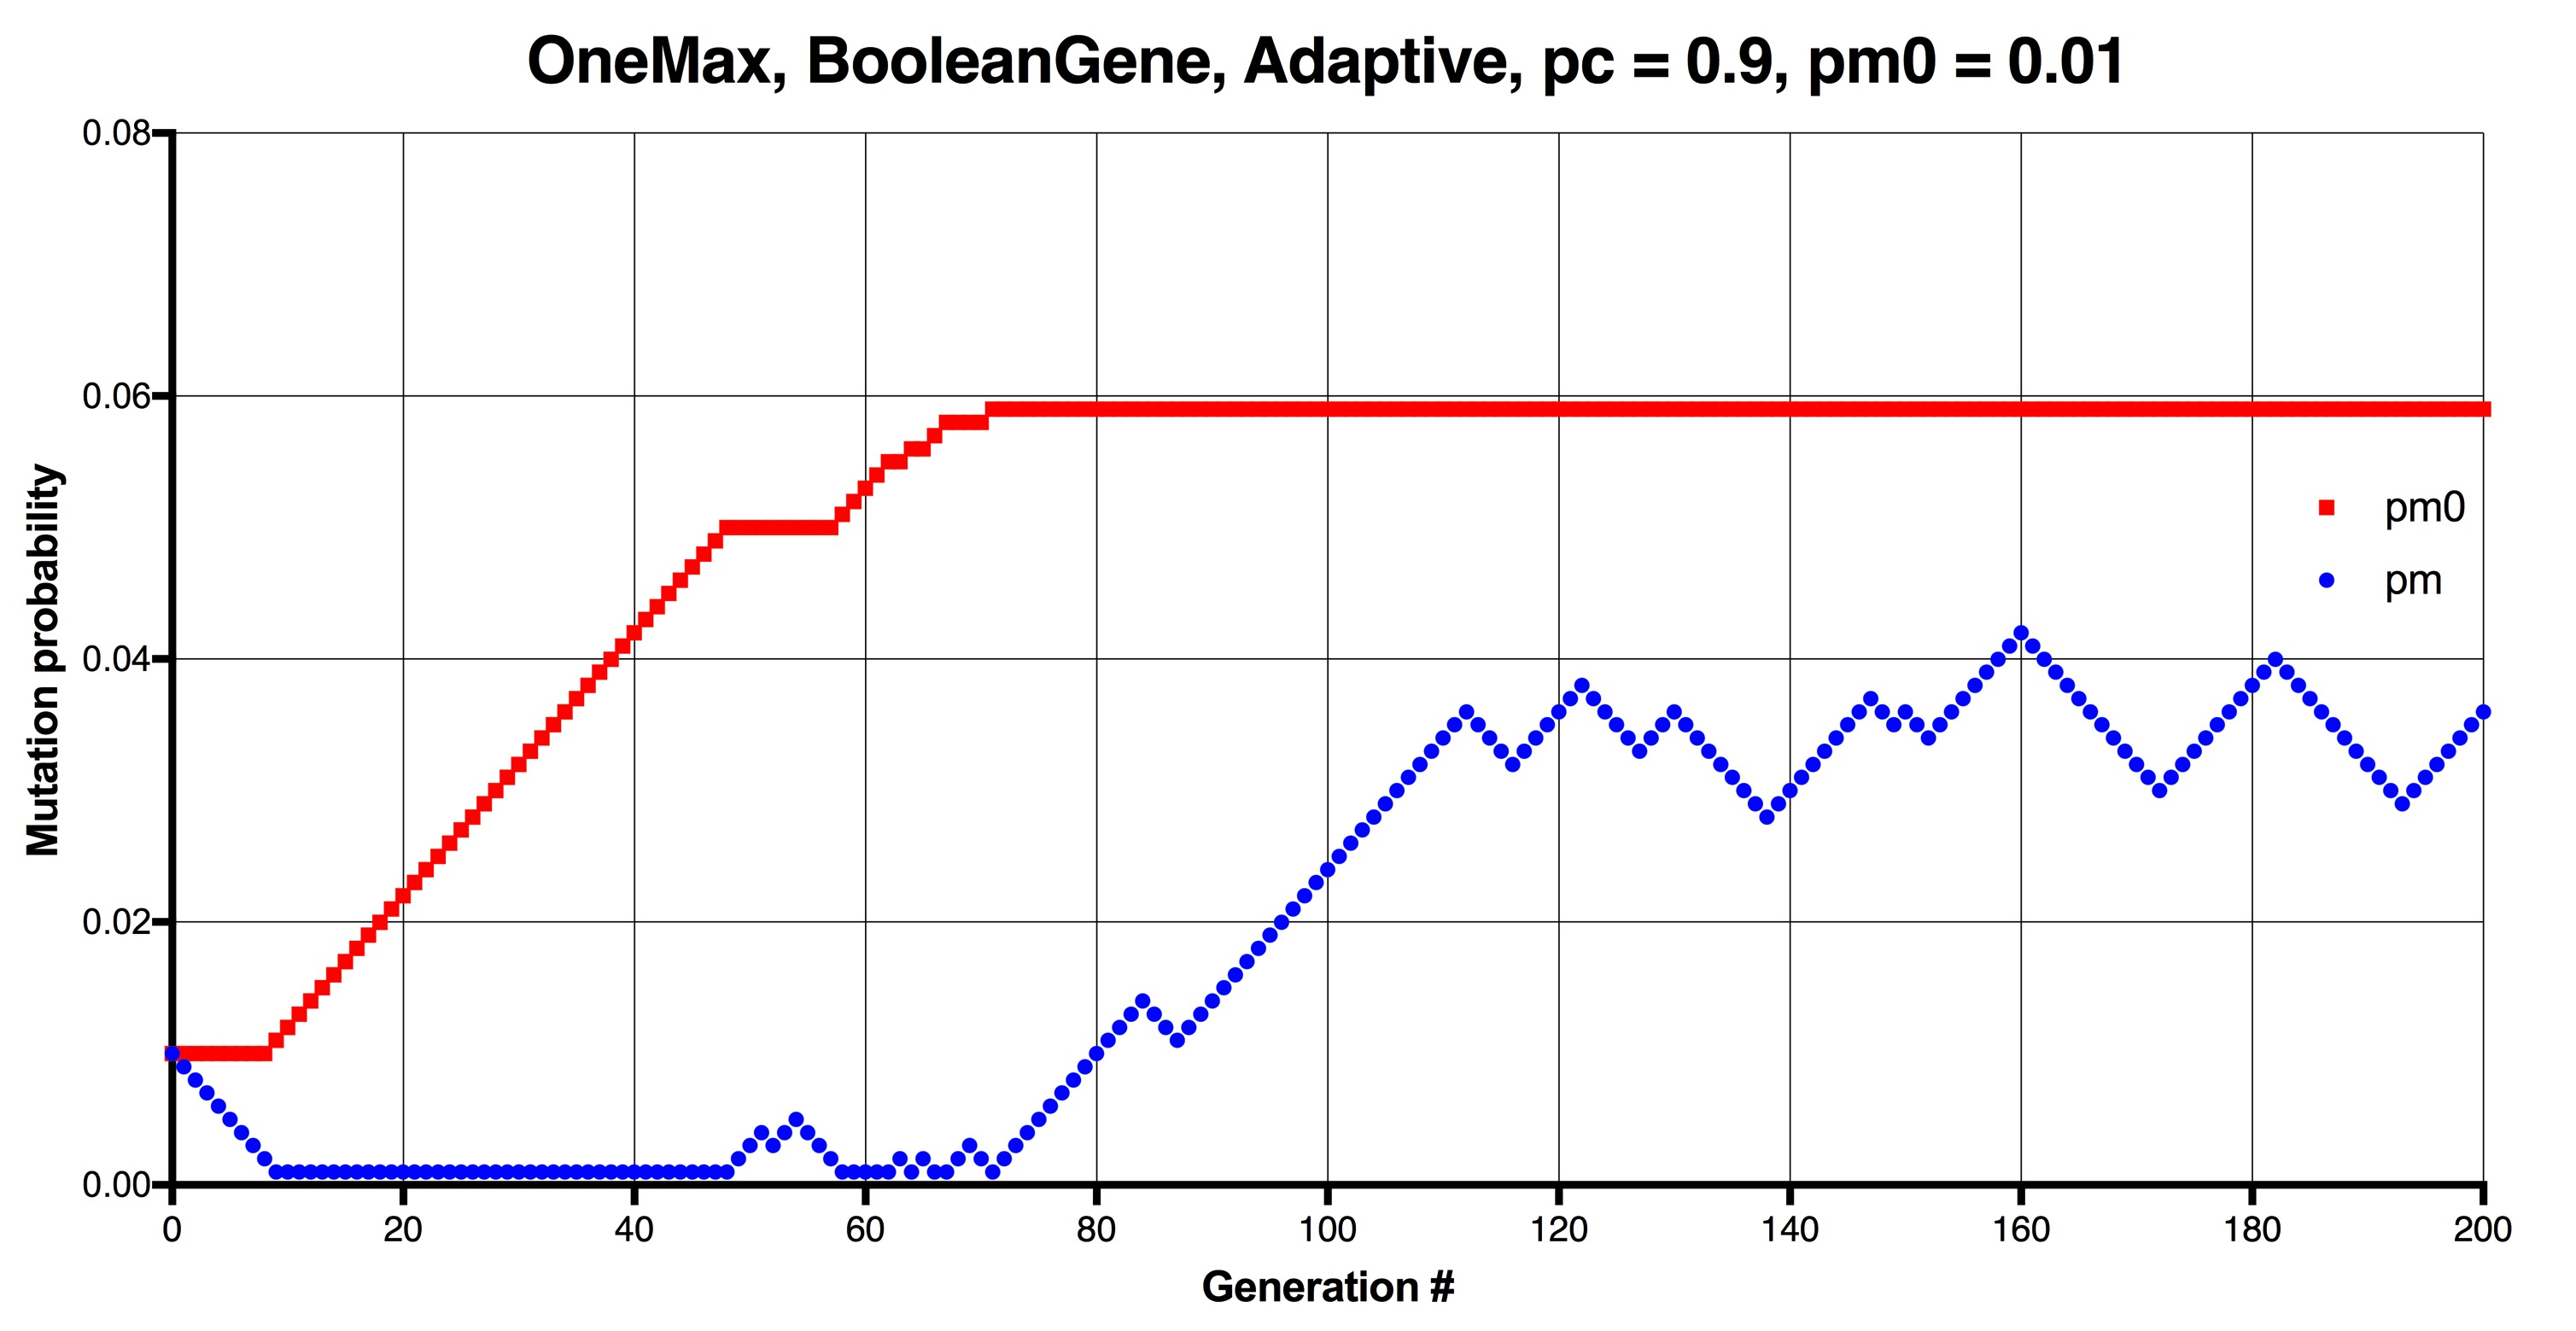
\includegraphics[width=1.0\textwidth]{onemax_boolean_adaptive_pm.jpg}
    \caption{Evolução da probabilidade de mutação $p_m$ ao longo das gerações, juntamente com o desvio do melhor valor de fitness com relação à média ($p_c=0.9$, ${p_m}_0=0.01$).}
    \label{fig:onemax_boolean_adaptive_pm}
\end{figure}

Por conta disso, ${p_m}_0$ começou a aumentar enquanto a população evoluía e ficava mais homogênea. O AGA, para uma população homogênea, interpreta isso como se a população tivesse travado em uma solução. Por conta disso, após cerca de 70 gerações, a homogeneização da população e o aumento de ${p_m}_0$ se encontraram, e $p_m$ começou a aumentar.

Quando $p_m$ parou de crescer (por volta de 110 gerações), ele estabilizou em torno de um valor mais alto que o inicial (por volta de 0.03). Tal aumento (tanto de $p_m$ quanto de ${p_m}_0$) se mostrou suficiente para que a população fosse incapaz de convergir conjuntamente para a solução ótima.

Foi possível tirar desta simulação que, mesmo que o intuito inicial deste AGA tivesse sido o de fugir de momentos em que o AG travasse em uma solução, ele veio com um custo, que foi o de evitar que a população fosse capaz de convergir conjuntamente para a solução ótima. Se o intuito de usar o AG for o de encontrar uma boa solução no final, esse custo é baixo.

Os dados de interesse vindos destas simulações podem ser encontrados na tabela \ref{tab:onemax_boolean}.

\begin{table}
\caption{Dados coletados do problema do OneMax Booleano ($p_m = 0.01$).}
\label{tab:onemax_boolean}

\center
\begin{tabular}{|c|cc|}
	\hline
	Algoritmo analisado (AG = caso estático)	& AG		& AGA		\\
	\hline
	Solução ótima encontrada?					& Sim		& Sim		\\
	Gerações p/solução ótima					& $78$		& $140$		\\
	Convergência da população (gerações)		& $93$		& $--$		\\
	Fitness médio após 100 gerações				& $100$		& $82.67$	\\
	Fitness médio após 200 gerações 			& $100$		& $99.17$	\\
	Valor final de $p_m$						& $0.01$ 	& $0.019$	\\
	Valor mínimo de $p_m$						& $0.01$	& $0.001$	\\
	Valor máximo de $p_m$						& $0.01$	& $0.021$	\\
	Valor médio de $p_m$						& $0.01$	& $0.00594$	\\
	Valor médio de $p_m$ (últimas 100 gerações)	& $0.01$	& $0.0105$	\\
	\hline
\end{tabular}
\end{table}

\section{OneMax Real}

Para o OneMax Real, é virtualmente impossível chegar ao valor máximo de fitness (100.0), uma vez que a mutação para um número aleatório trabalha no intervalo [0, 1). Por conta disso, as análises feitas aqui focaram no comportamento da curva e na diferença de comportamento frente aos resultados do OneMax Booleano.

\subsection{Caso Estático}

Para o OneMax Real, foi possível ver, na figura \ref{fig:onemax_real}, que a população, mesmo não sendo capaz de atingir o fitness máximo, conseguiu se homogeneizar e continuar crescendo ao longo das gerações, o que foi demonstrado também pela queda do desvio padrão.

\begin{figure}[ht!]
    \centering 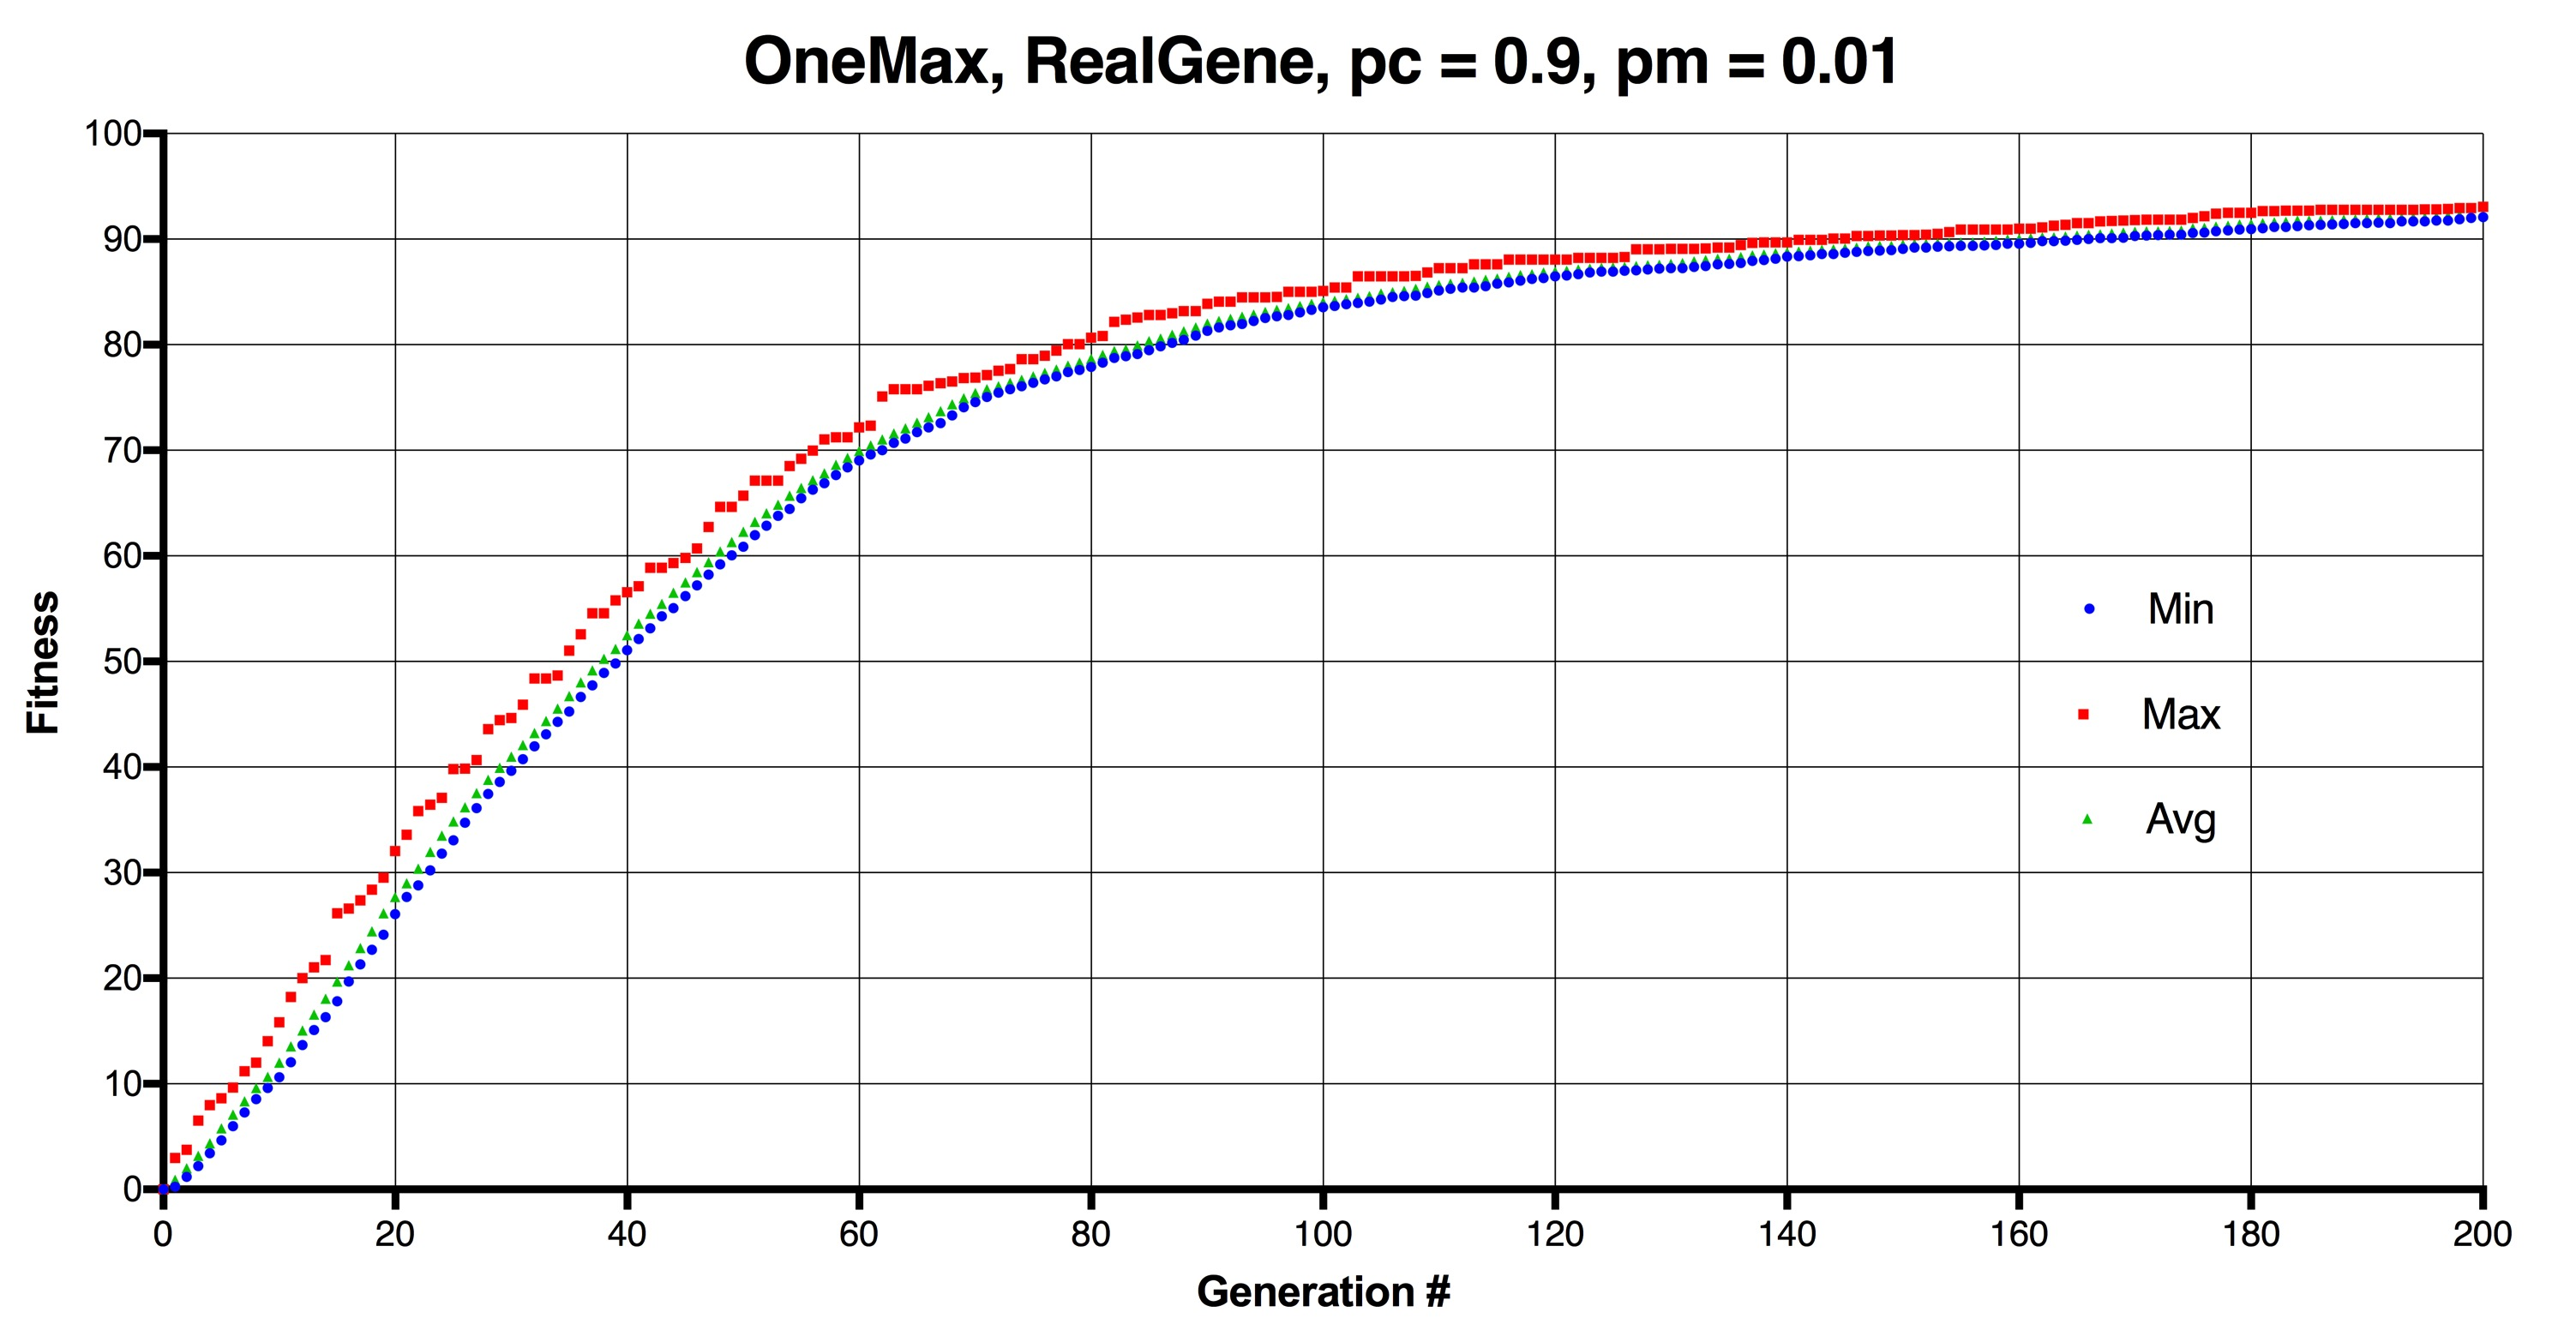
\includegraphics[width=1.0\textwidth]{onemax_real.jpg}
    \caption{Evolução do fitness para o problema do OneMax Real mostrando mínimo, máximo e valor médio ($p_c=0.9$, $p_m=0.01$).}
    \label{fig:onemax_real}
\end{figure}

Os pontos de qualquer uma das medições (média, mínimo e máximo) parecem formar uma curva. Descobri-la fugiu do escopo deste trabalho, mas tal formato pode estar associado à probabilidade de se aumentar a expressividade de um gene. Na execução deste AG, cada gene é levado para mutação com probabilidade $p_m$. Se um gene tiver uma expressividade $0 < x < 1$, a mutação (assumida uniforme) possui uma probabilidade $(1-x)$ de aumentá-la. Logo, a expressividade aumentará em uma dada geração com probabilidade:

\begin{equation}
	p_m(1-x)
\end{equation}

\subsection{Caso Adaptativo}

Os efeitos notados para o OneMax Booleano se repetiram aqui. Como se pode ver nas figuras \ref{fig:onemax_real_adaptive}, a população se estabilizou após cerca de 110 gerações, o que indica que a mutação se estabilizou em um determinado valor.

\begin{figure}[ht!]
    \centering 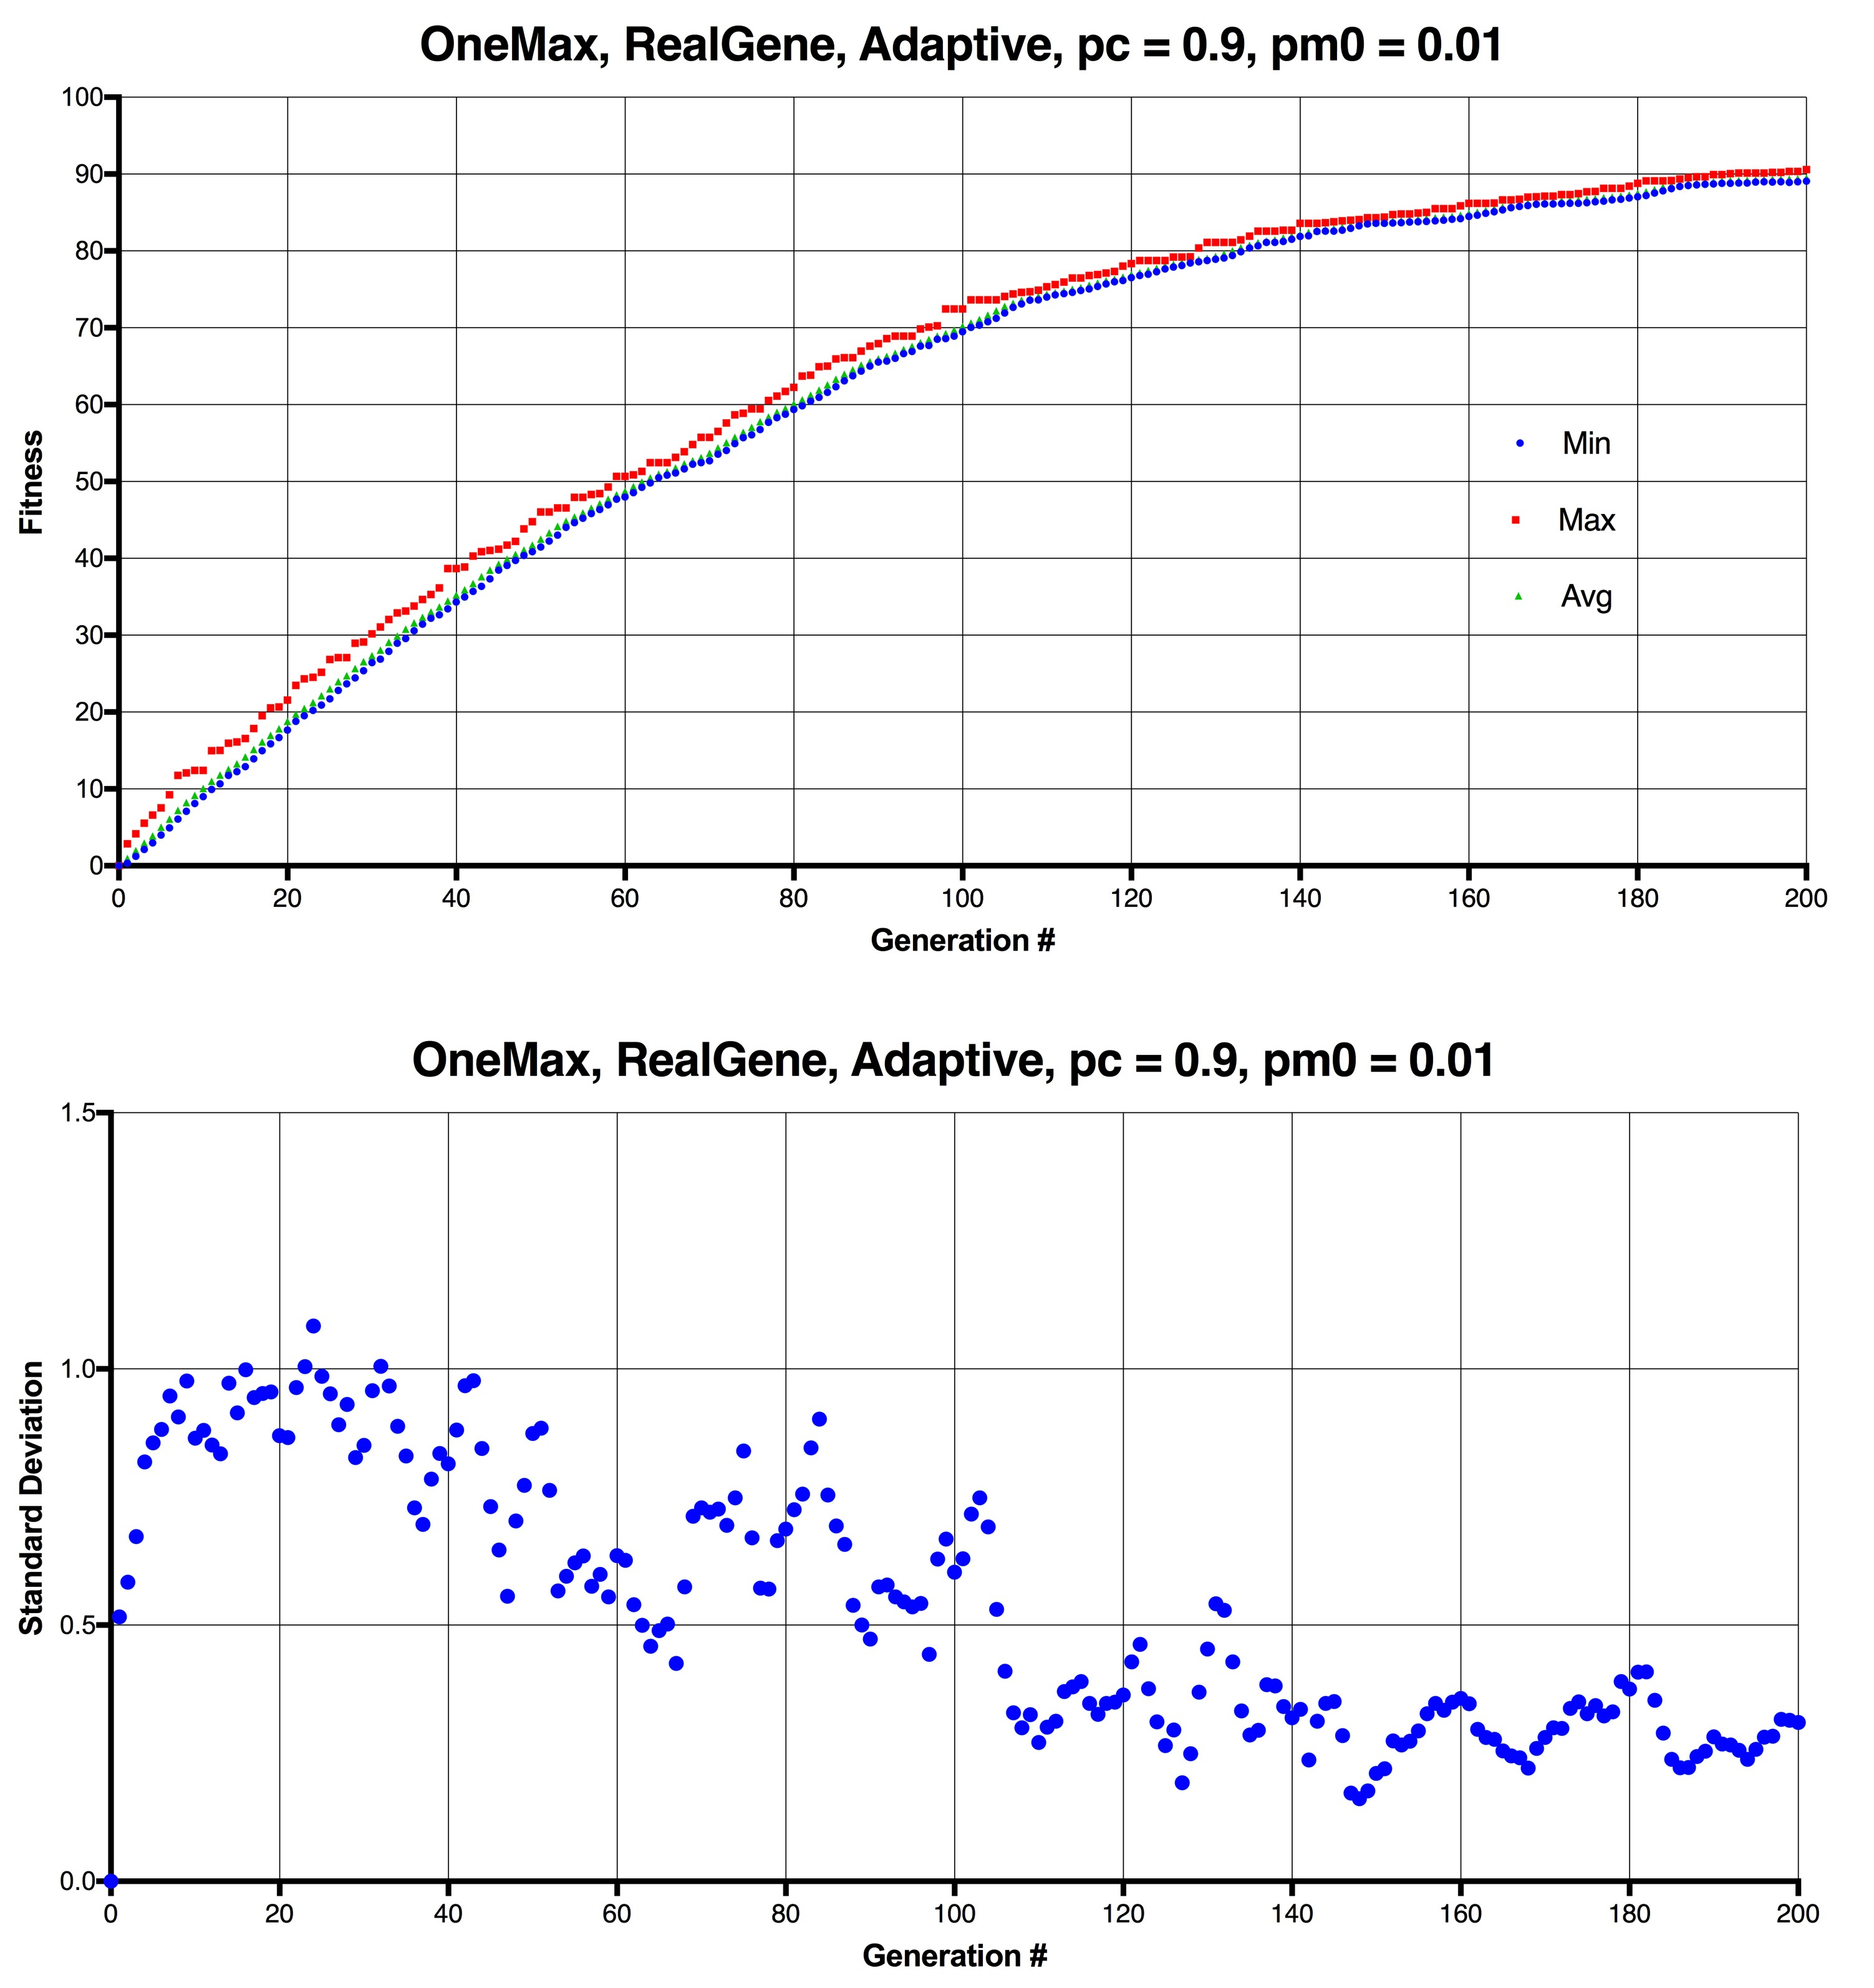
\includegraphics[width=1.0\textwidth]{onemax_real_adaptive.jpg}
    \caption{Evolução do fitness para o problema do OneMax Real Adaptativo mostrando mínimo, máximo e valor médio ($p_c=0.9$, ${p_m}_0=0.01$).}
    \label{fig:onemax_real_adaptive}
\end{figure}

Vemos também que o desvio padrão dos valores de fitness aparentou crescer ao longo das gerações. Isso se deu mais por conta do aumento de $p_m$ após 73 gerações, mostrado na figura \ref{fig:onemax_real_adaptive_pm}. Comparado ao OneMax Booleano, o $p_m$ atingiu valores maiores próximo às últimas gerações (oscilando em torno de 0.04), o que pode ter contribuído para o aumento do desvio padrão, mesmo com a média dos valores de fitness se mantendo relativamente no mesmo valor.

\begin{figure}[ht!]
    \centering 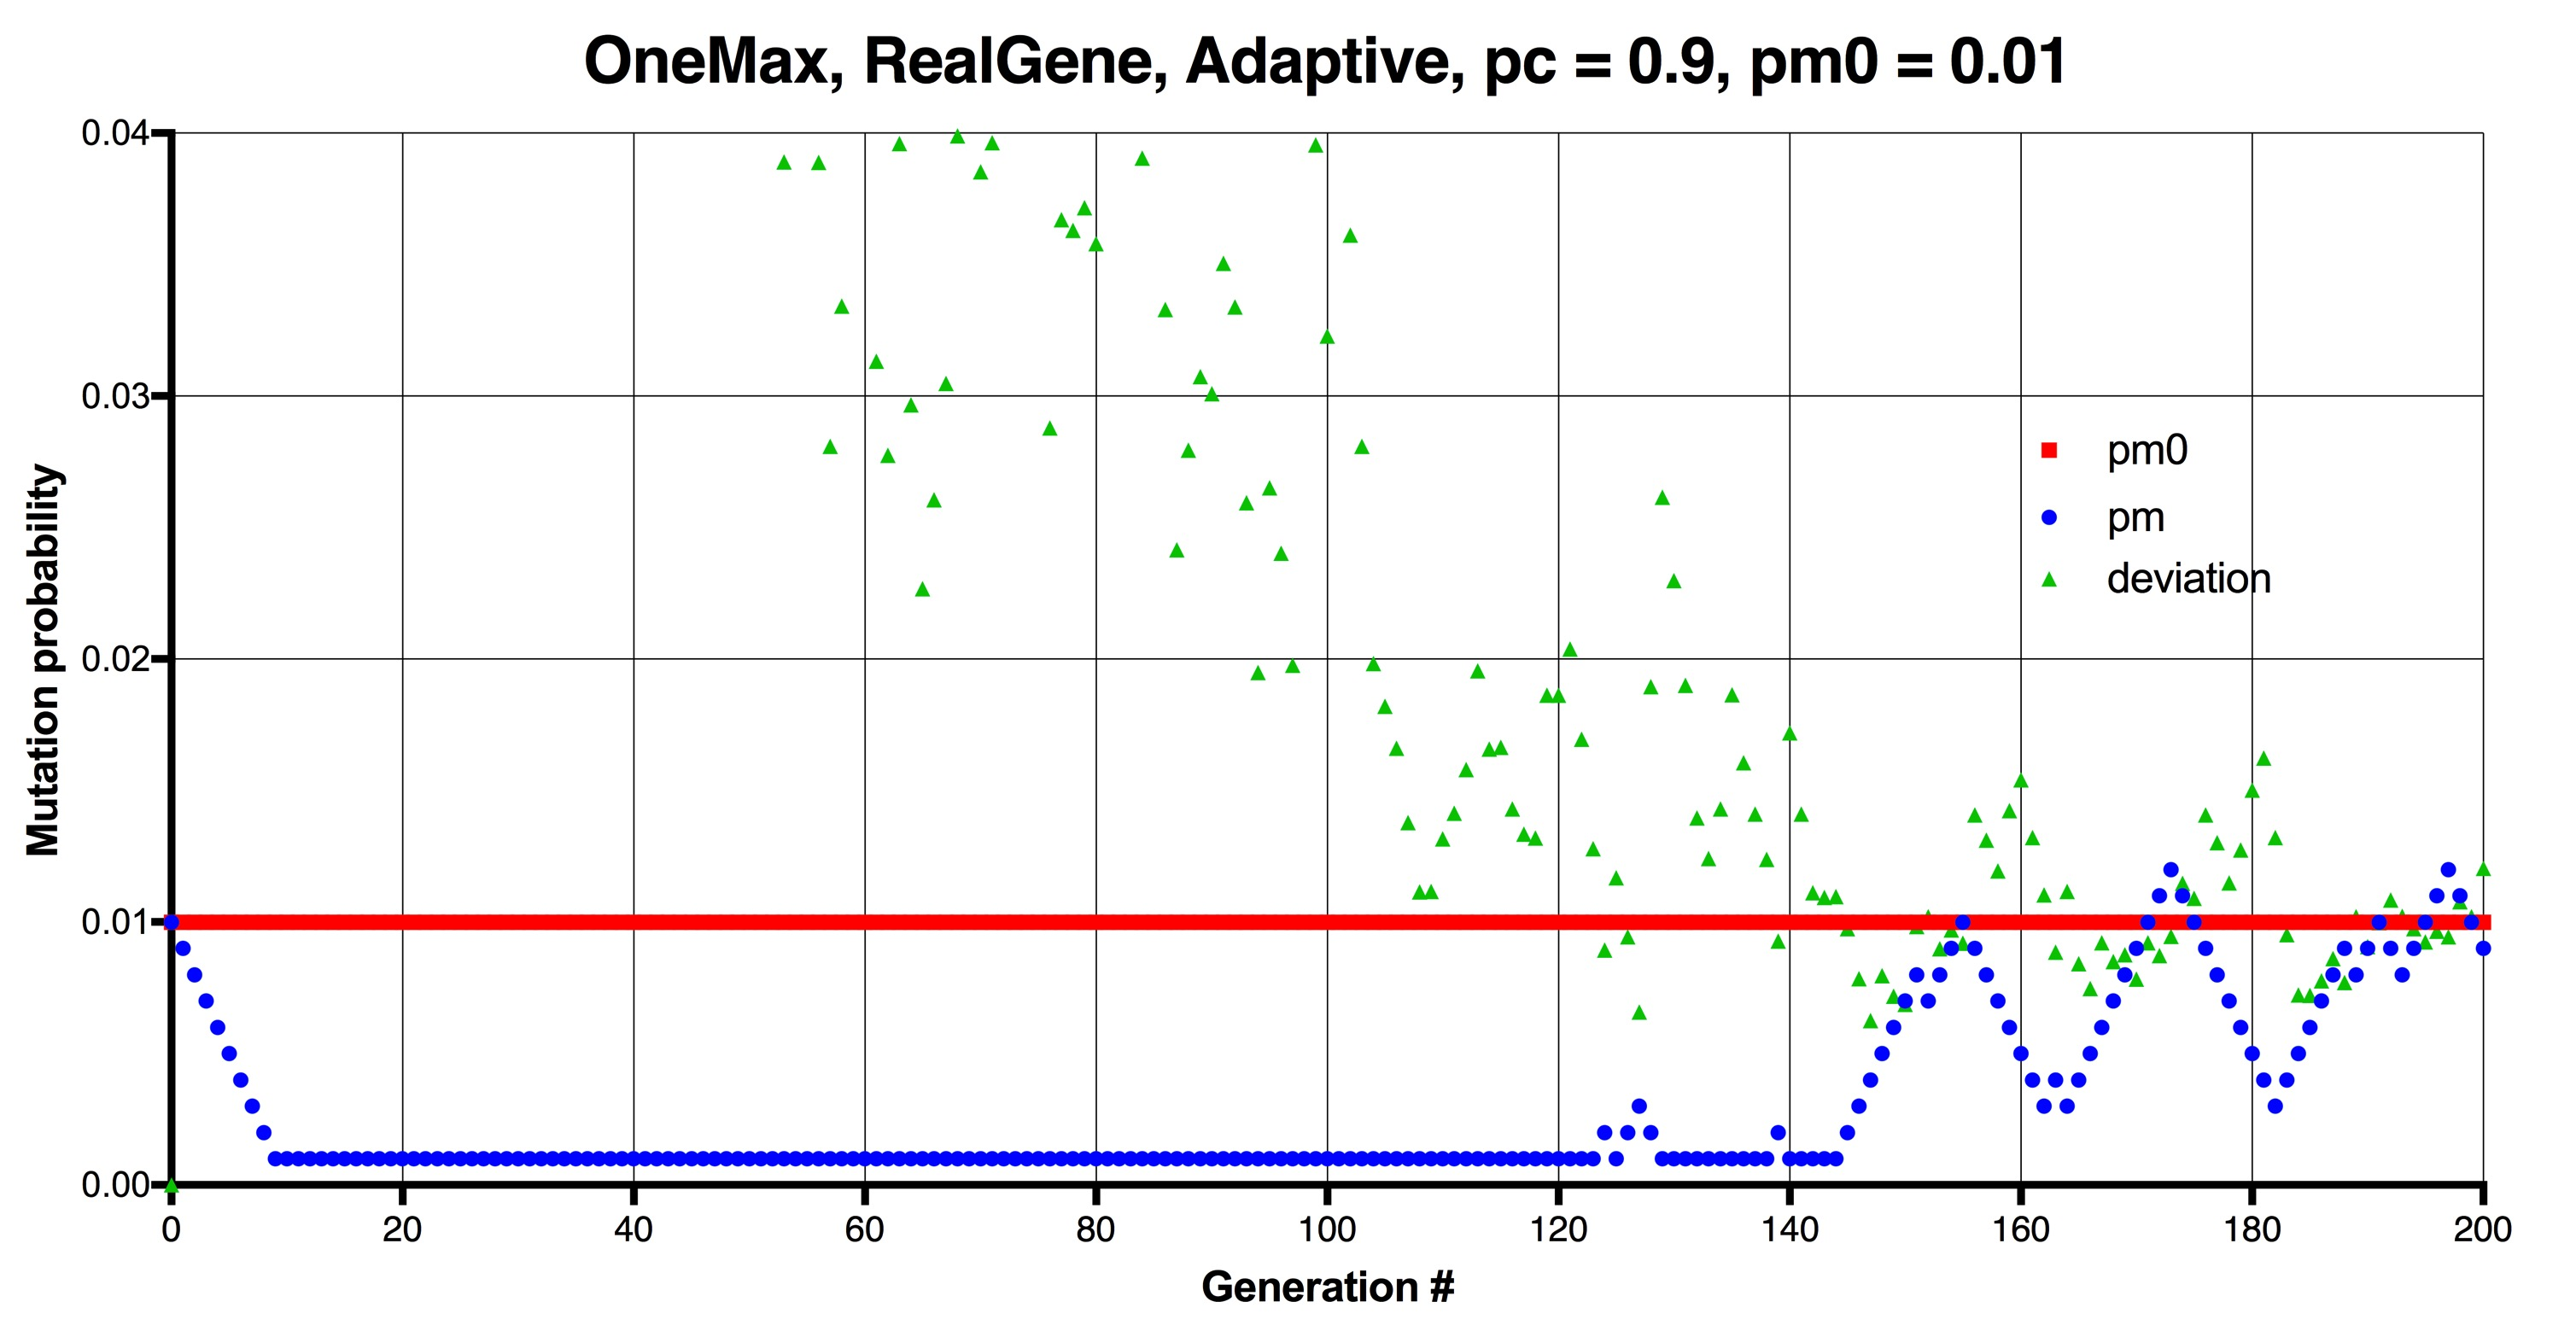
\includegraphics[width=1.0\textwidth]{onemax_real_adaptive_pm.jpg}
    \caption{Probabilidade de mutação ao longo das gerações para o problema do OneMax Real Adaptativo ($p_c=0.9$, ${p_m}_0=0.01$).}
    \label{fig:onemax_real_adaptive_pm}
\end{figure}

Os dados de interesse vindos destas simulações podem ser encontrados na tabela  \ref{tab:onemax_real}.

\begin{table}
\caption{Dados coletados do problema do OneMax Real ($p_m = 0.01$).}
\label{tab:onemax_real}

\center
\begin{tabular}{|c|cc|}
	\hline
	Algoritmo analisado (AG = caso estático) 	& AG		& AGA		\\
	\hline
	Fitness máximo após 100 gerações			& $85.115$	& $72.452$	\\
	Fitness médio após 100 gerações				& $84.048$	& $70.186$	\\
	Fitness máximo após 200 gerações 			& $93.083$	& $90.585$	\\
	Fitness médio após 200 gerações 			& $92.355$	& $89.507$	\\
	Valor final de $p_m$						& $0.01$ 	& $0.009$	\\
	Valor mínimo de $p_m$						& $0.01$	& $0.001$	\\
	Valor máximo de $p_m$						& $0.01$	& $0.012$	\\
	Valor médio de $p_m$						& $0.01$	& $0.00300$	\\
	Valor médio de $p_m$ (últimas 100 gerações)	& $0.01$	& $0.00458$	\\
	\hline
\end{tabular}
\end{table}

\section{Caixeiro Viajante Adaptado}

Para as simulações deste problema, utilizou-se então o grafo do programa Open-Source DEAP com 17 cidades \cite{DEAP_JMLR2012, deap2016tsp}. Tal grafo é conexo, completo e bidirecionado, e sua distância mínima (começando na primeira cidade) é 2085. Ele está presente na listagem \ref{lst:cidades}.

\begin{lstlisting}[float, floatplacement=H, caption={Mapa de cidades para o problema do Caixeiro Viajante Adaptado.}, label=lst:cidades]
[0, 633, 257, 91, 412, 150, 80, 134, 259, 505, 353, 324, 70, 211, 268, 246, 121],
[633, 0, 390, 661, 227, 488, 572, 530, 555, 289, 282, 638, 567, 466, 420, 745, 518],
[257, 390, 0, 228, 169, 112, 196, 154, 372, 262, 110, 437, 191, 74, 53, 472, 142],
[91, 661, 228, 0, 383, 120, 77, 105, 175, 476, 324, 240, 27, 182, 239, 237, 84],
[412, 227, 169, 383, 0, 267, 351, 309, 338, 196, 61, 421, 346, 243, 199, 528, 297],
[150, 488, 112, 120, 267, 0, 63, 34, 264, 360, 208, 329, 83, 105, 123, 364, 35],
[80, 572, 196, 77, 351, 63, 0, 29, 232, 444, 292, 297, 47, 150, 207, 332, 29],
[134, 530, 154, 105, 309, 34, 29, 0, 249, 402, 250, 314, 68, 108, 165, 349, 36],
[259, 555, 372, 175, 338, 264, 232, 249, 0, 495, 352, 95, 189, 326, 383, 202, 236],
[505, 289, 262, 476, 196, 360, 444, 402, 495, 0, 154, 578, 439, 336, 240, 685, 390],
[353, 282, 110, 324, 61, 208, 292, 250, 352, 154, 0, 435, 287, 184, 140, 542, 238],
[324, 638, 437, 240, 421, 329, 297, 314, 95, 578, 435, 0, 254, 391, 448, 157, 301],
[70, 567, 191, 27, 346, 83, 47, 68, 189, 439, 287, 254, 0, 145, 202, 289, 55],
[211, 466, 74, 182, 243, 105, 150, 108, 326, 336, 184, 391, 145, 0, 57, 426, 96],
[268, 420, 53, 239, 199, 123, 207, 165, 383, 240, 140, 448, 202, 57, 0, 483, 153],
[246, 745, 472, 237, 528, 364, 332, 349, 202, 685, 542, 157, 289, 426, 483, 0, 336],
[121, 518, 142, 84, 297, 35, 29, 36, 236, 390, 238, 301, 55, 96, 153, 336, 0]
\end{lstlisting}

\subsection{Caso Estático ($p_m = 0.01$)}

Para o caso estático com $p_m = 0.01$, mostrado na figura \ref{fig:tsp001}, vemos que este valor de $p_m$ incentiva pouco o encontro de soluções melhores, demonstrado pela melhor solução (pontos azuis) ter mantido o mesmo valor por mais de 100 gerações. Em termos de desvio padrão, na figura \ref{fig:tsp001std}, percebeu-se que $p_m = 0.01$ foi capaz apenas de igualar os valores de fitness de modo rápido (uma vez que há apenas 15 genes a serem recombinados).

\begin{figure}[ht!]
    \centering 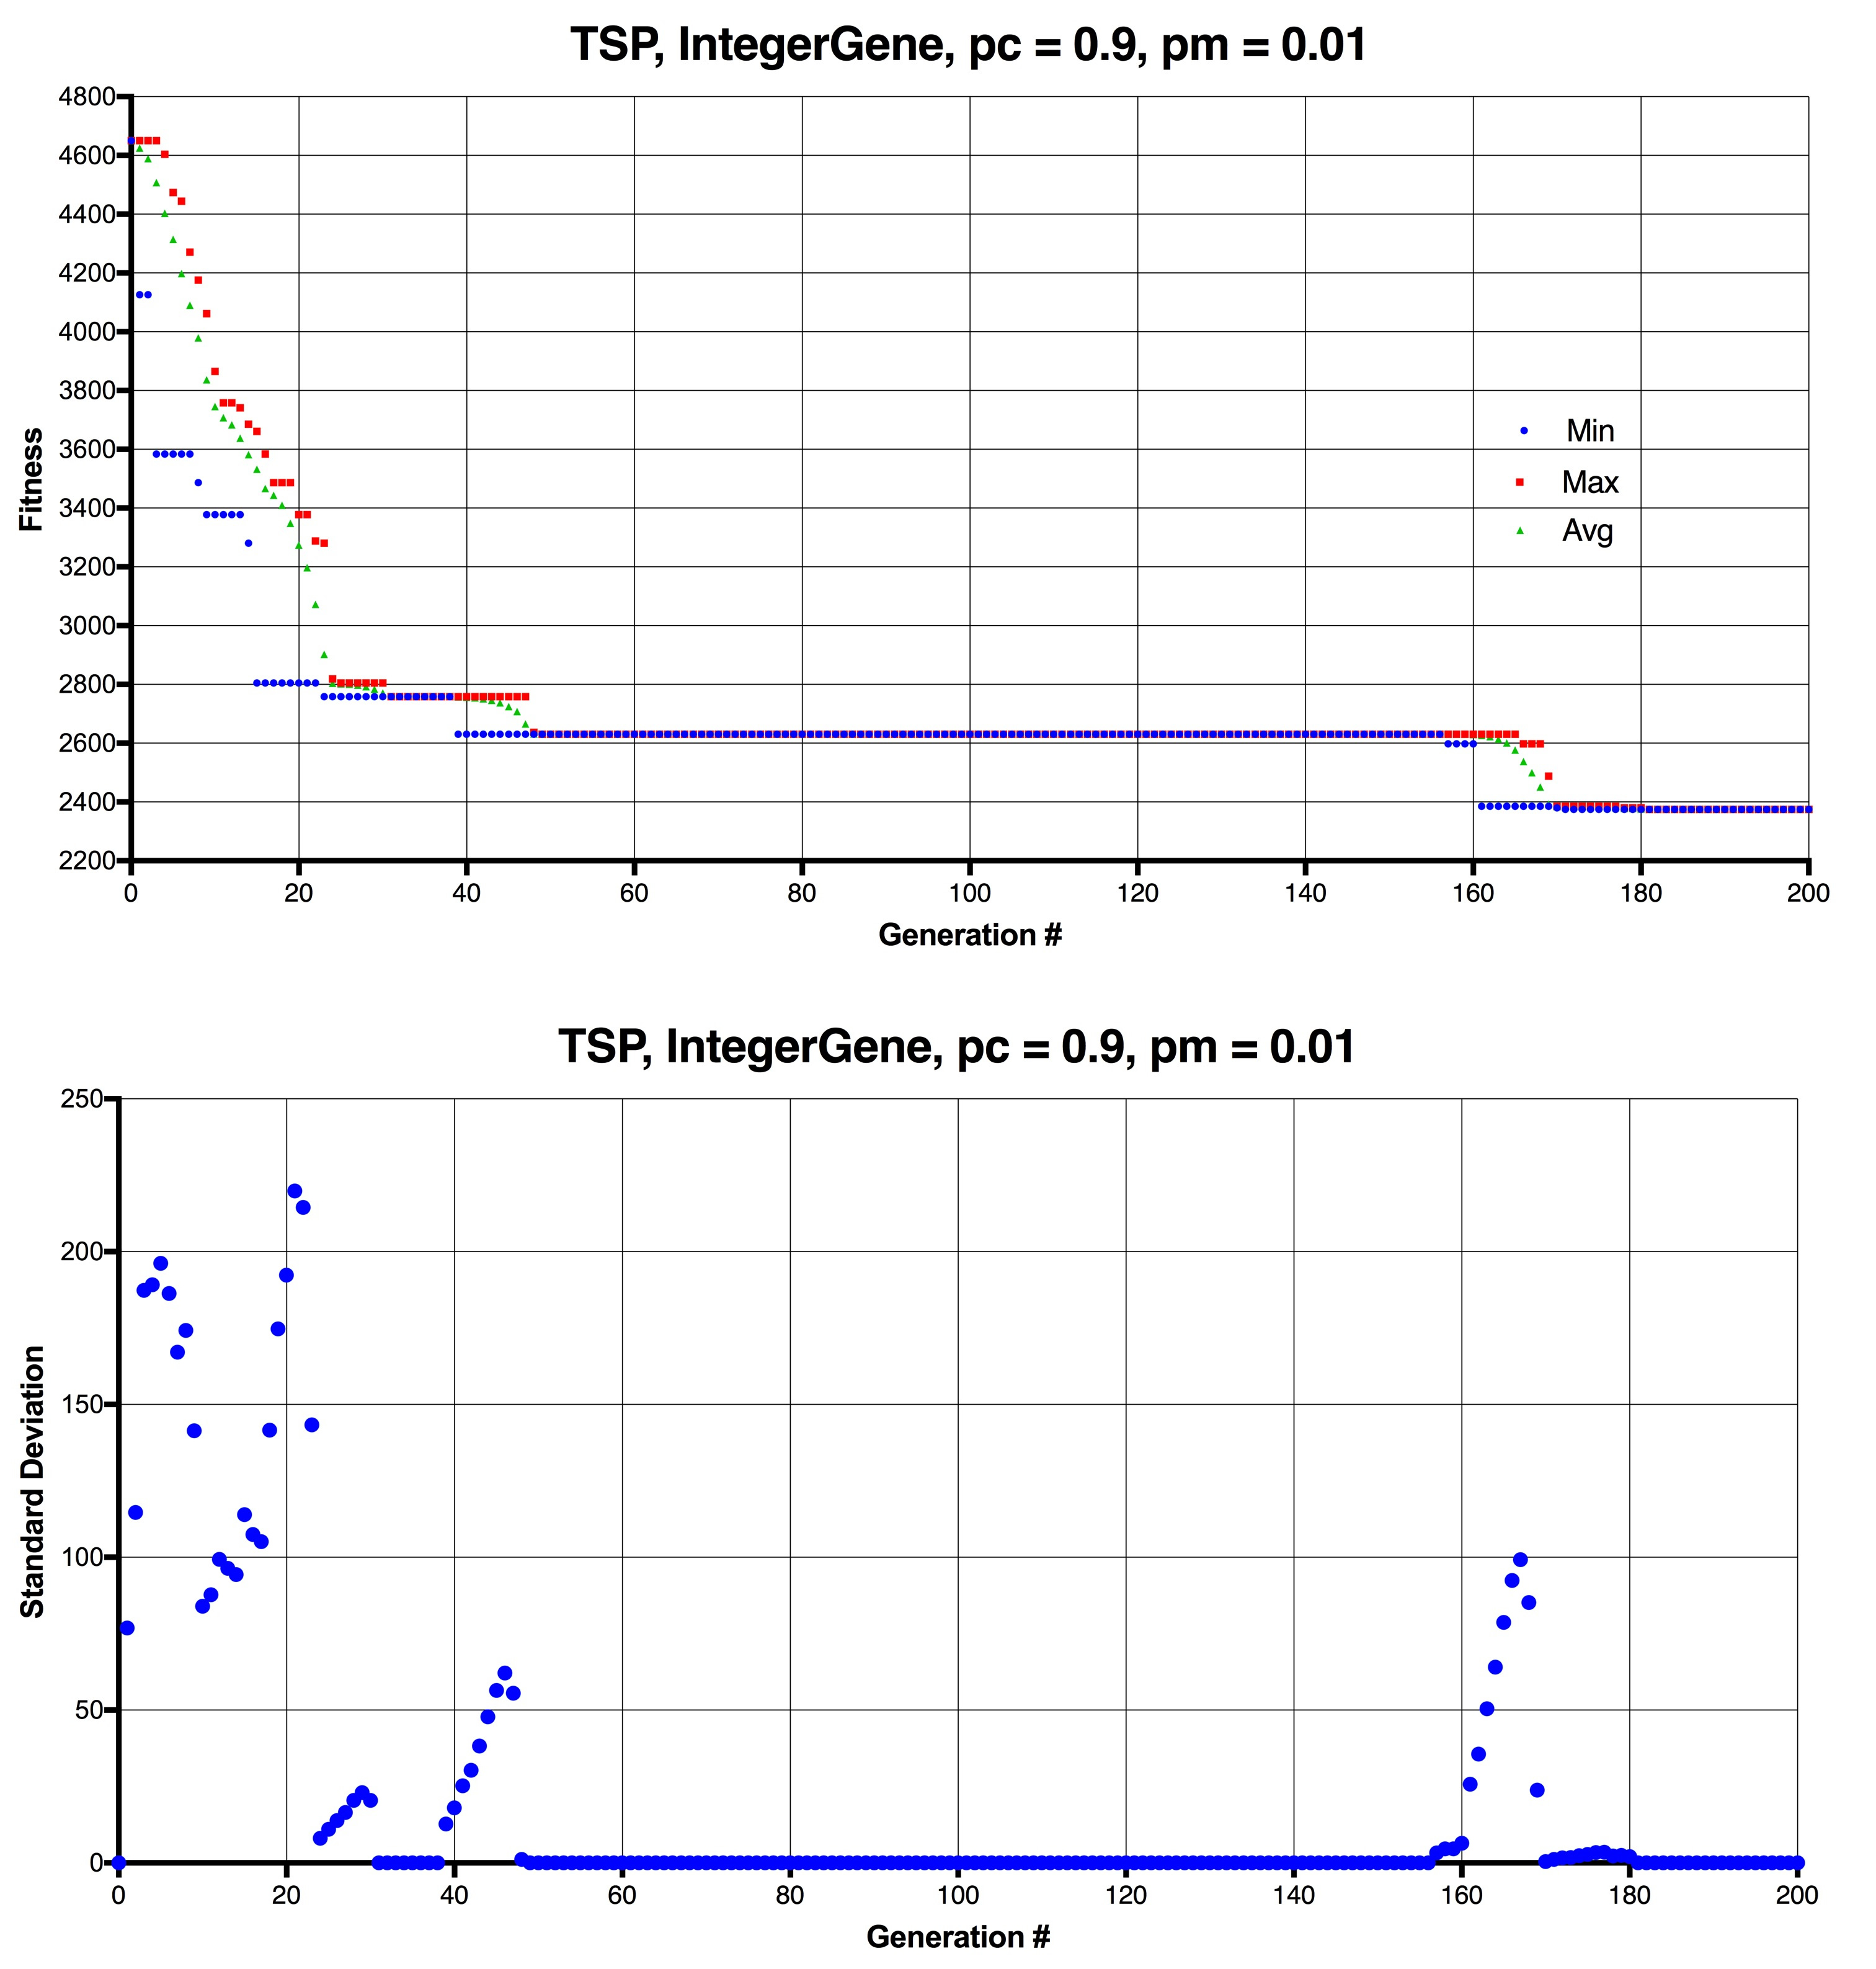
\includegraphics[width=1.0\textwidth]{tsp_001.jpg}
    \caption{Evolução do fitness para o problema do Caixeiro Viajante Adaptado mostrando mínimo, máximo e valor médio ($p_c=0.9$, $p_m=0.01$). O menor caminho encontrado tem distância total de 2375.}
    \label{fig:tsp001}
\end{figure}

\begin{figure}[ht!]
    \centering 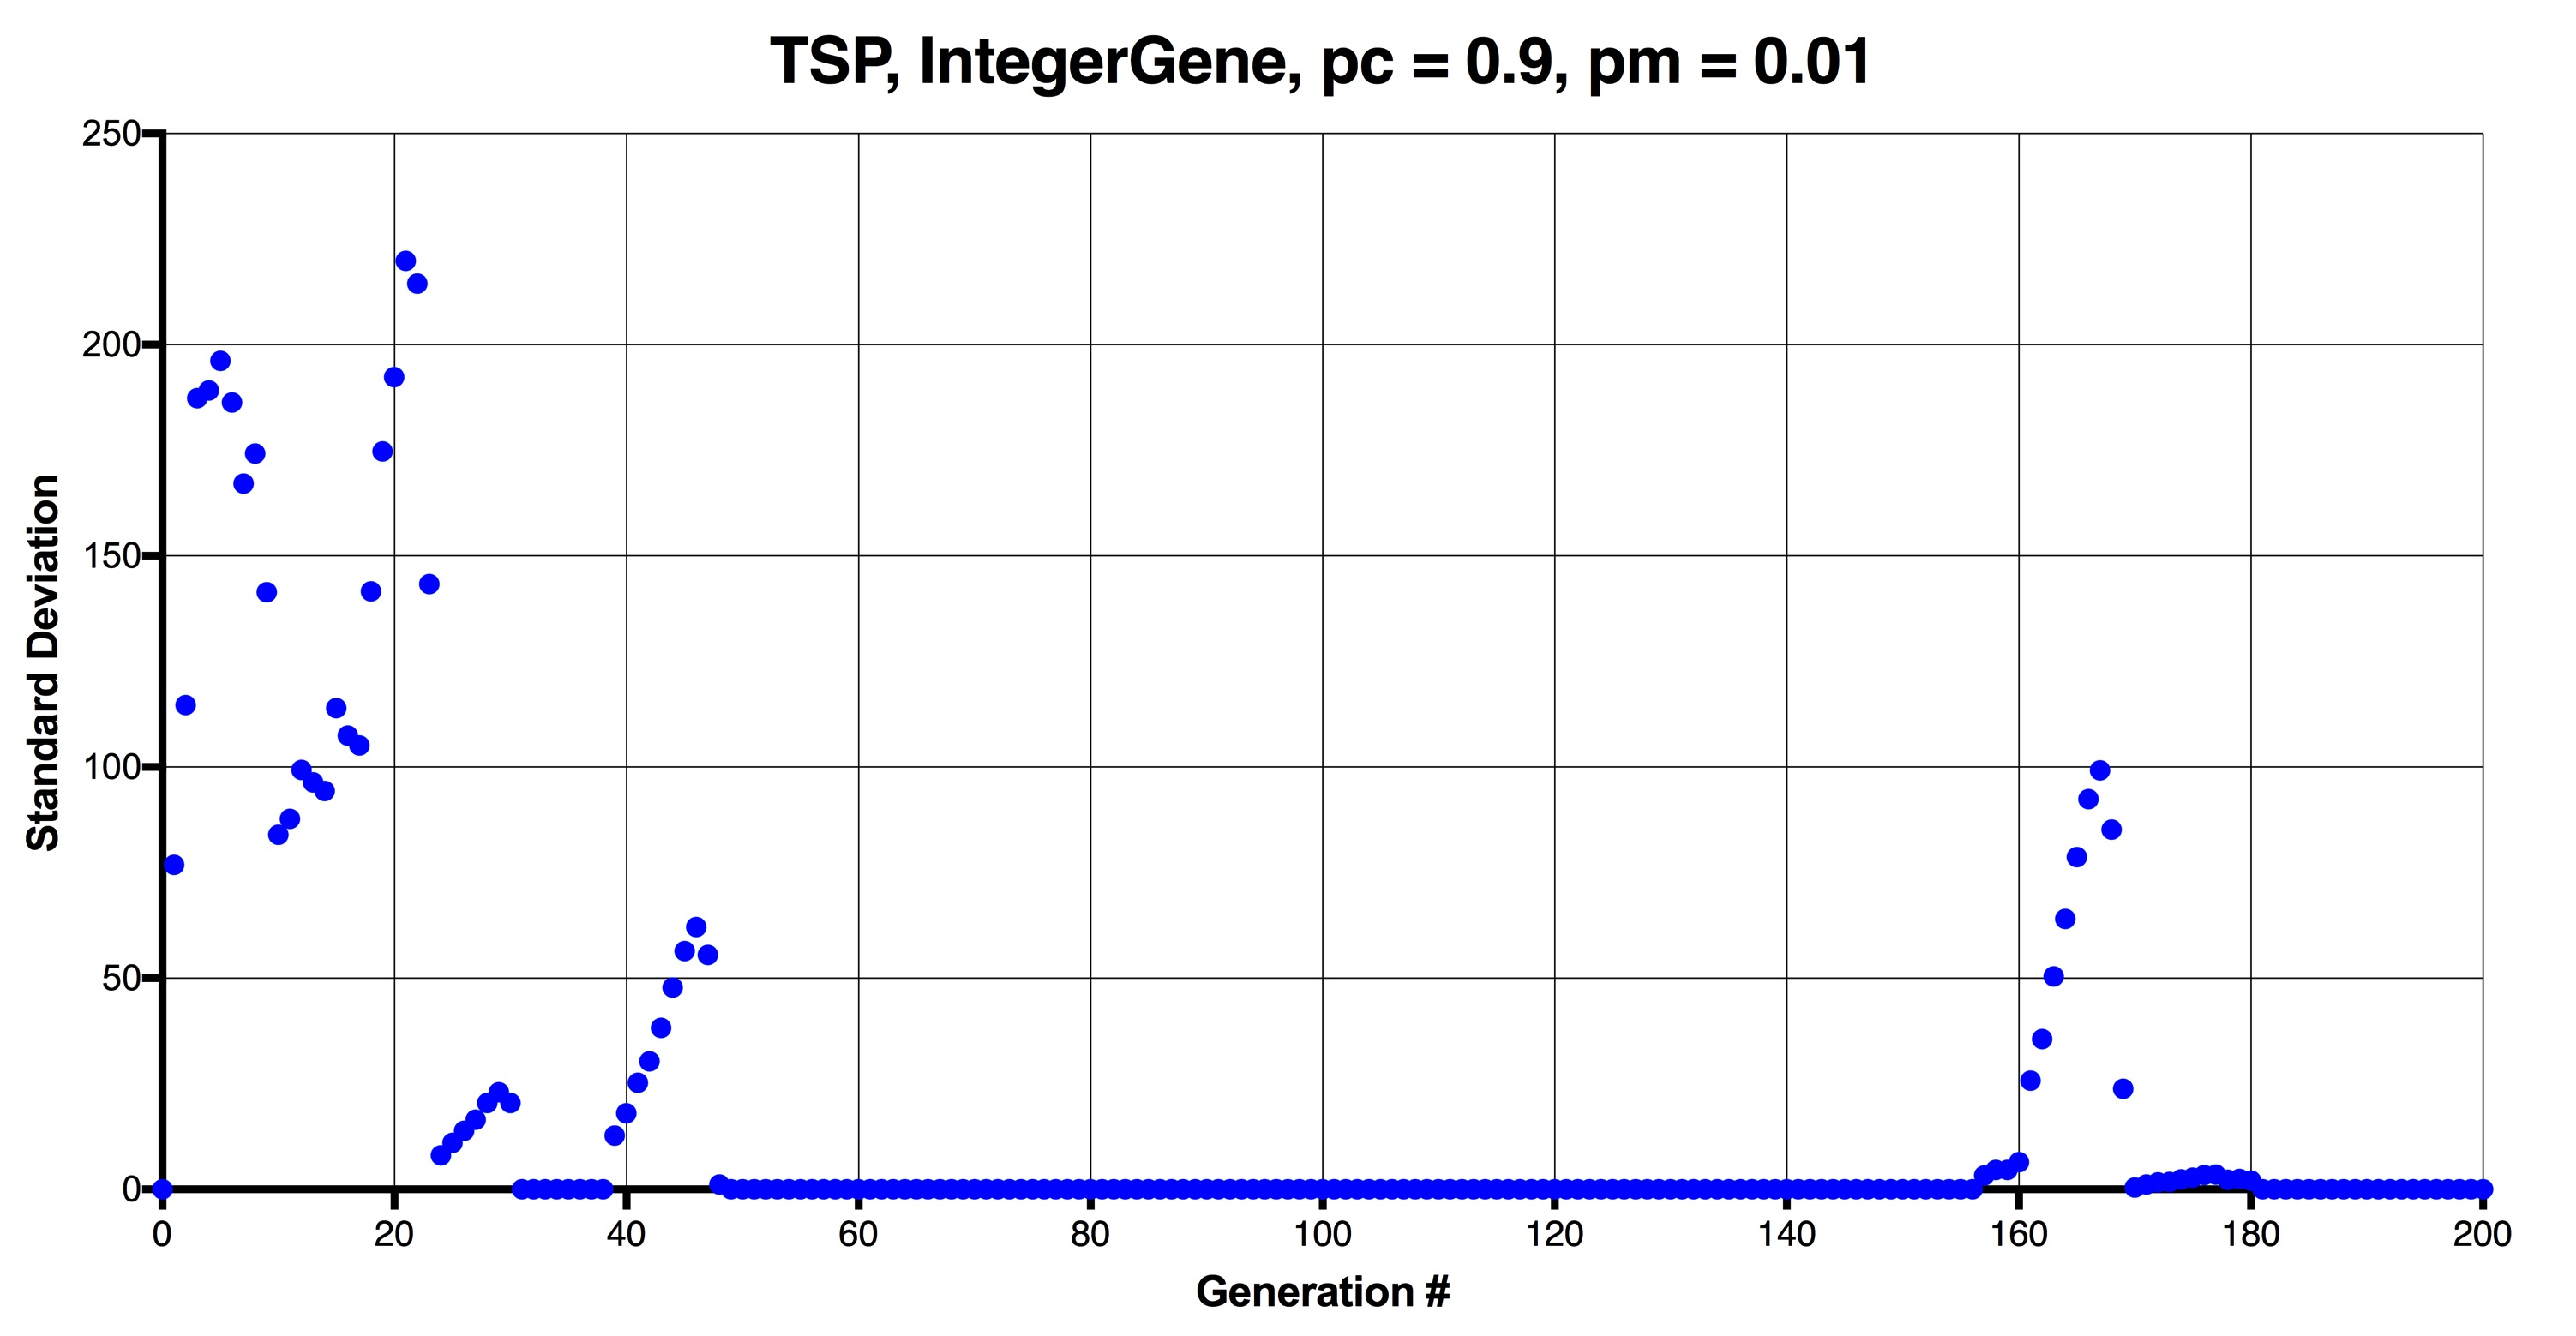
\includegraphics[width=1.0\textwidth]{tsp_001_std.jpg}
    \caption{Desvio padrão ao longo das gerações para o problema do Caixeiro Viajante Adaptado ($p_c=0.9$, ${p_m}_0=0.01$).}
    \label{fig:tsp001std}
\end{figure}

Uma possível interpretação foi a de que o AG travou em um mínimo local, e um valor maior de $p_m$ poderia resolver este problema. Optou-se então por testar $p_m = 0.2$.

\subsection{Caso Estático ($p_m = 0.2$)}

Para o caso estático com $p_m = 0.2$, mostrado na figura \ref{fig:tsp02}, vemos que $p_m = 0.2$ conseguiu chegar a uma solução melhor (2300 contra 2375). No entanto, o comportamento do valor mínimo de fitness ainda foi muito próximo daquele visto para $p_m = 0.01$ (agora mantendo a melhor solução por mais de 120 gerações).

\begin{figure}[ht!]
    \centering 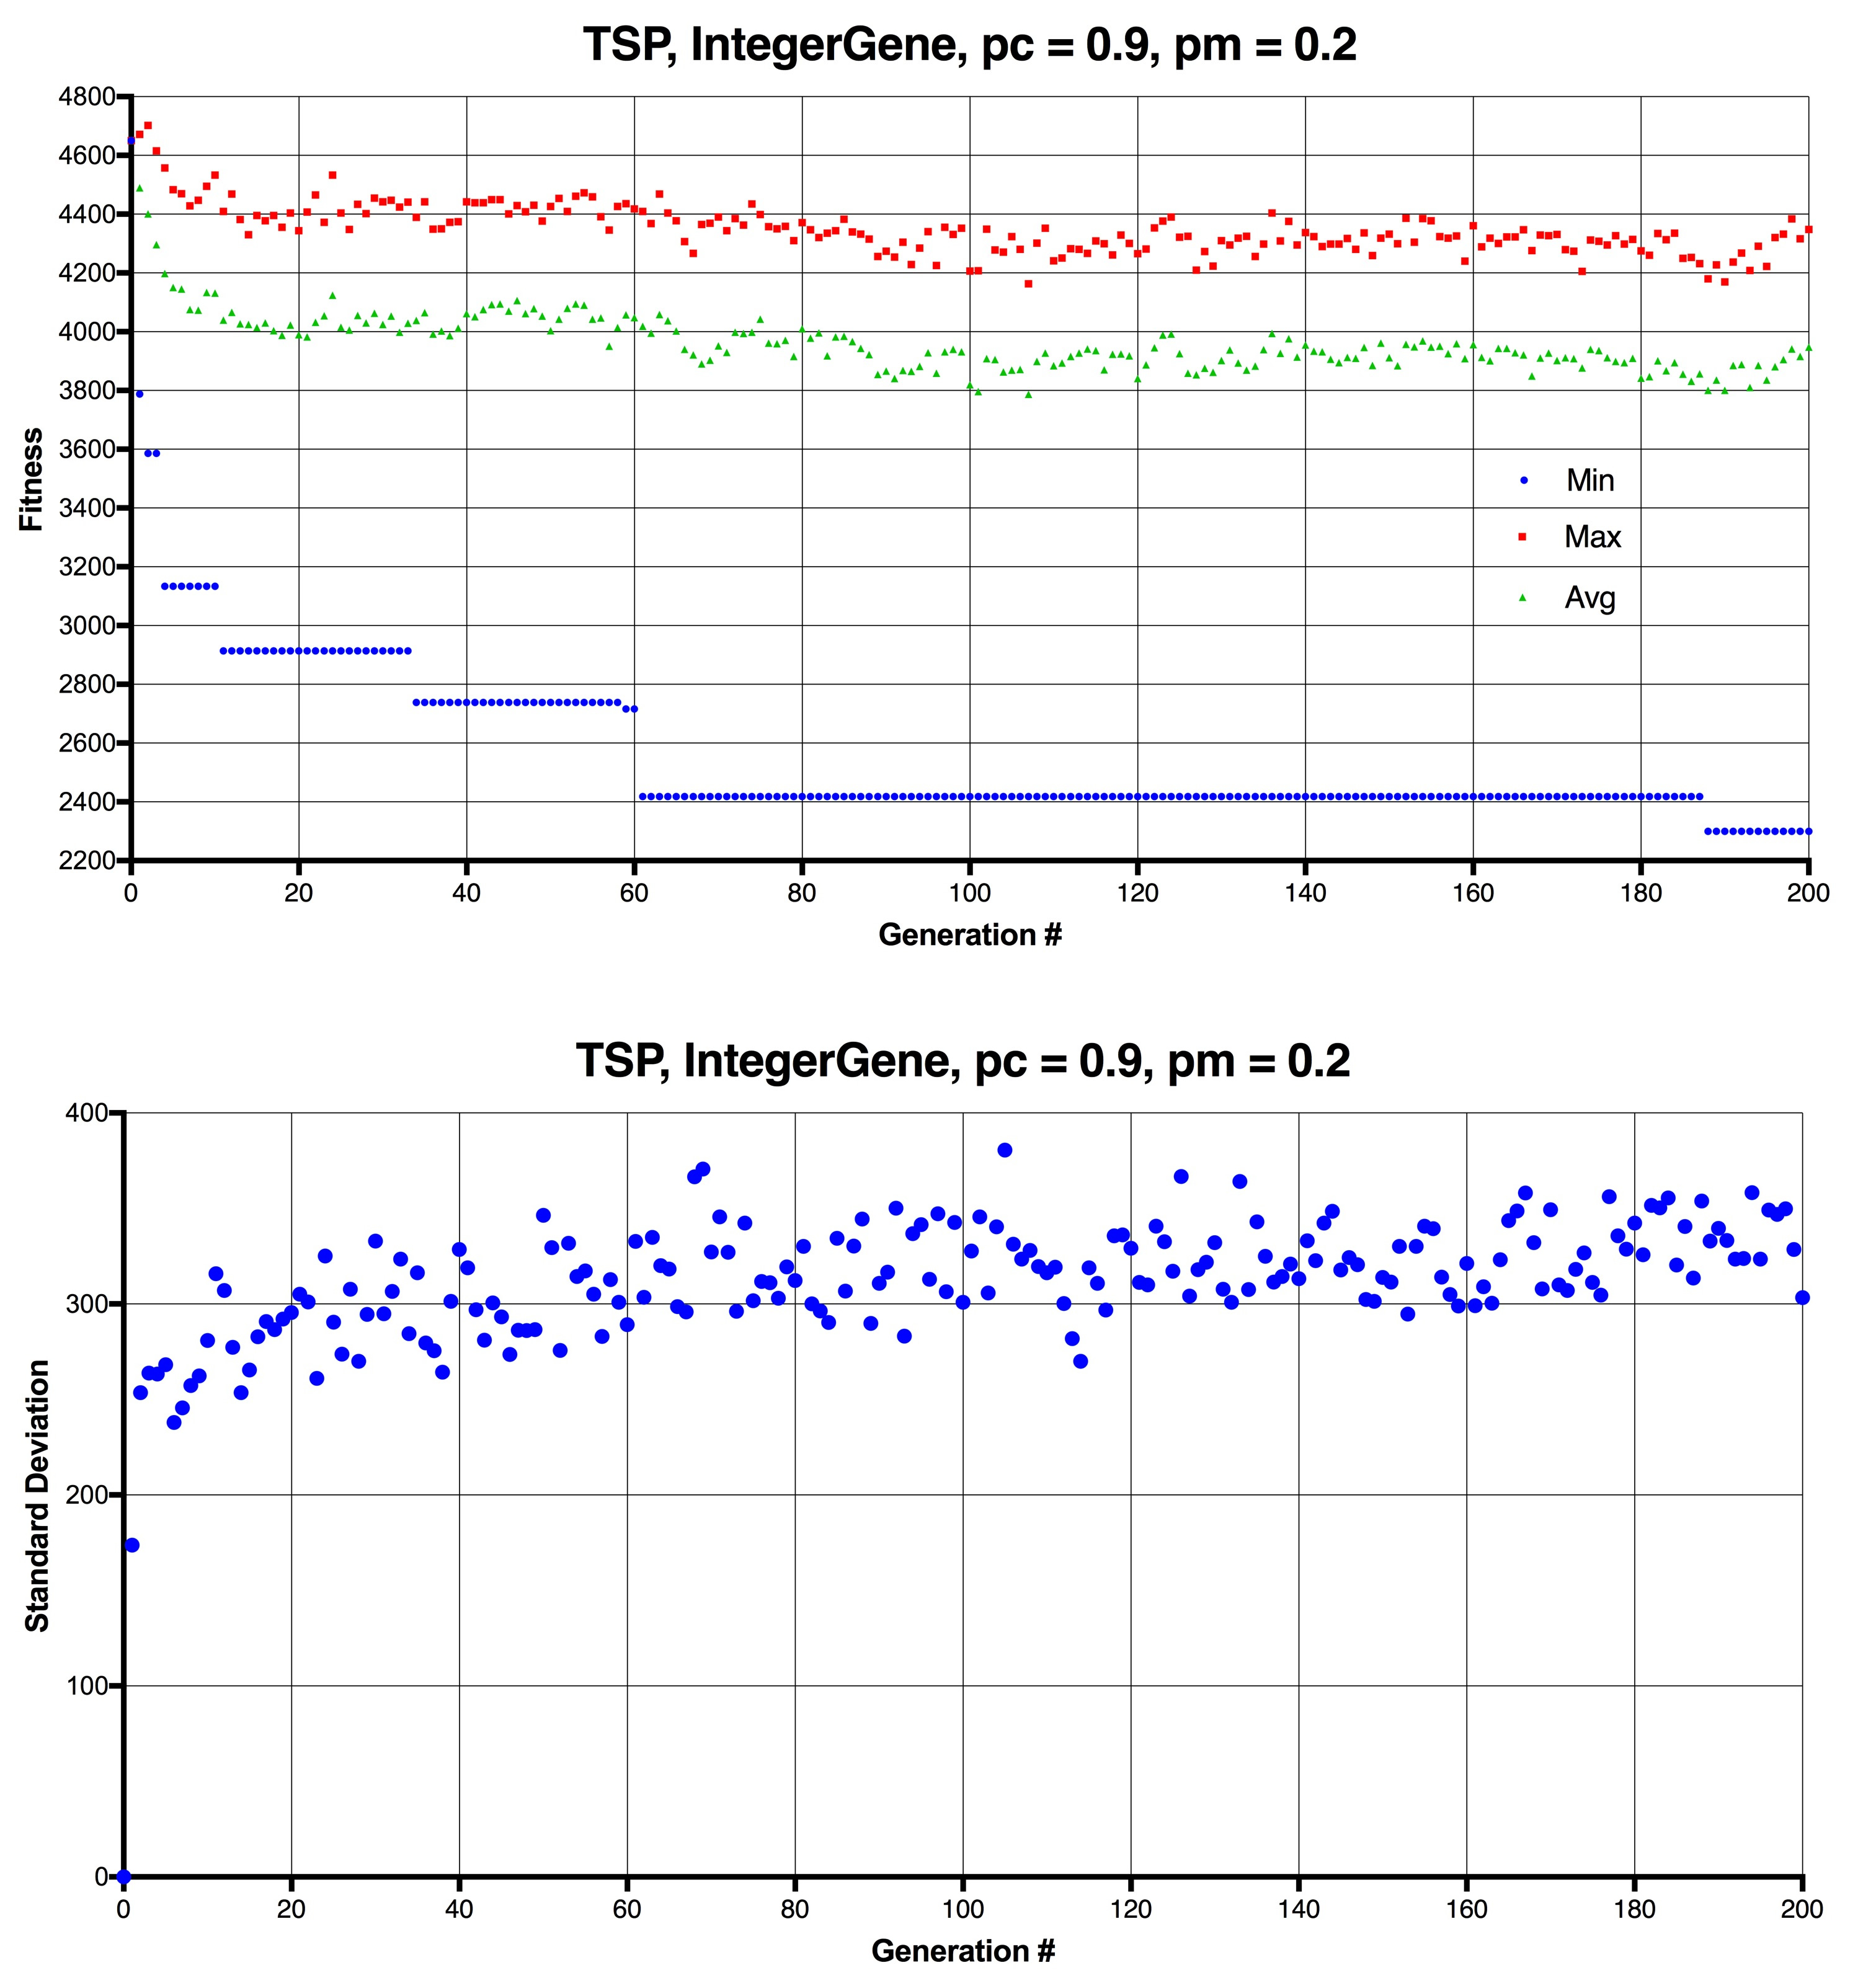
\includegraphics[width=1.0\textwidth]{tsp_02.jpg}
    \caption{Evolução do fitness para o problema do Caixeiro Viajante Adaptado mostrando mínimo, máximo e valor médio ($p_c=0.9$, $p_m=0.2$). O menor caminho encontrado tem distância total de 2300.}
    \label{fig:tsp02}
\end{figure}

O desvio padrão, mostrado na figura \ref{fig:tsp02std}, mostrou que uma mutação mais intensa incentiva o surgimento de muito mais soluções. No entanto, tais soluções são igualmente imprevisíveis aos olhos do problema, o que fez crer que aumentar $p_m$ (para 20\%, que já é absurdamente alto) não fez diferença para o caso estático.

\begin{figure}[ht!]
    \centering 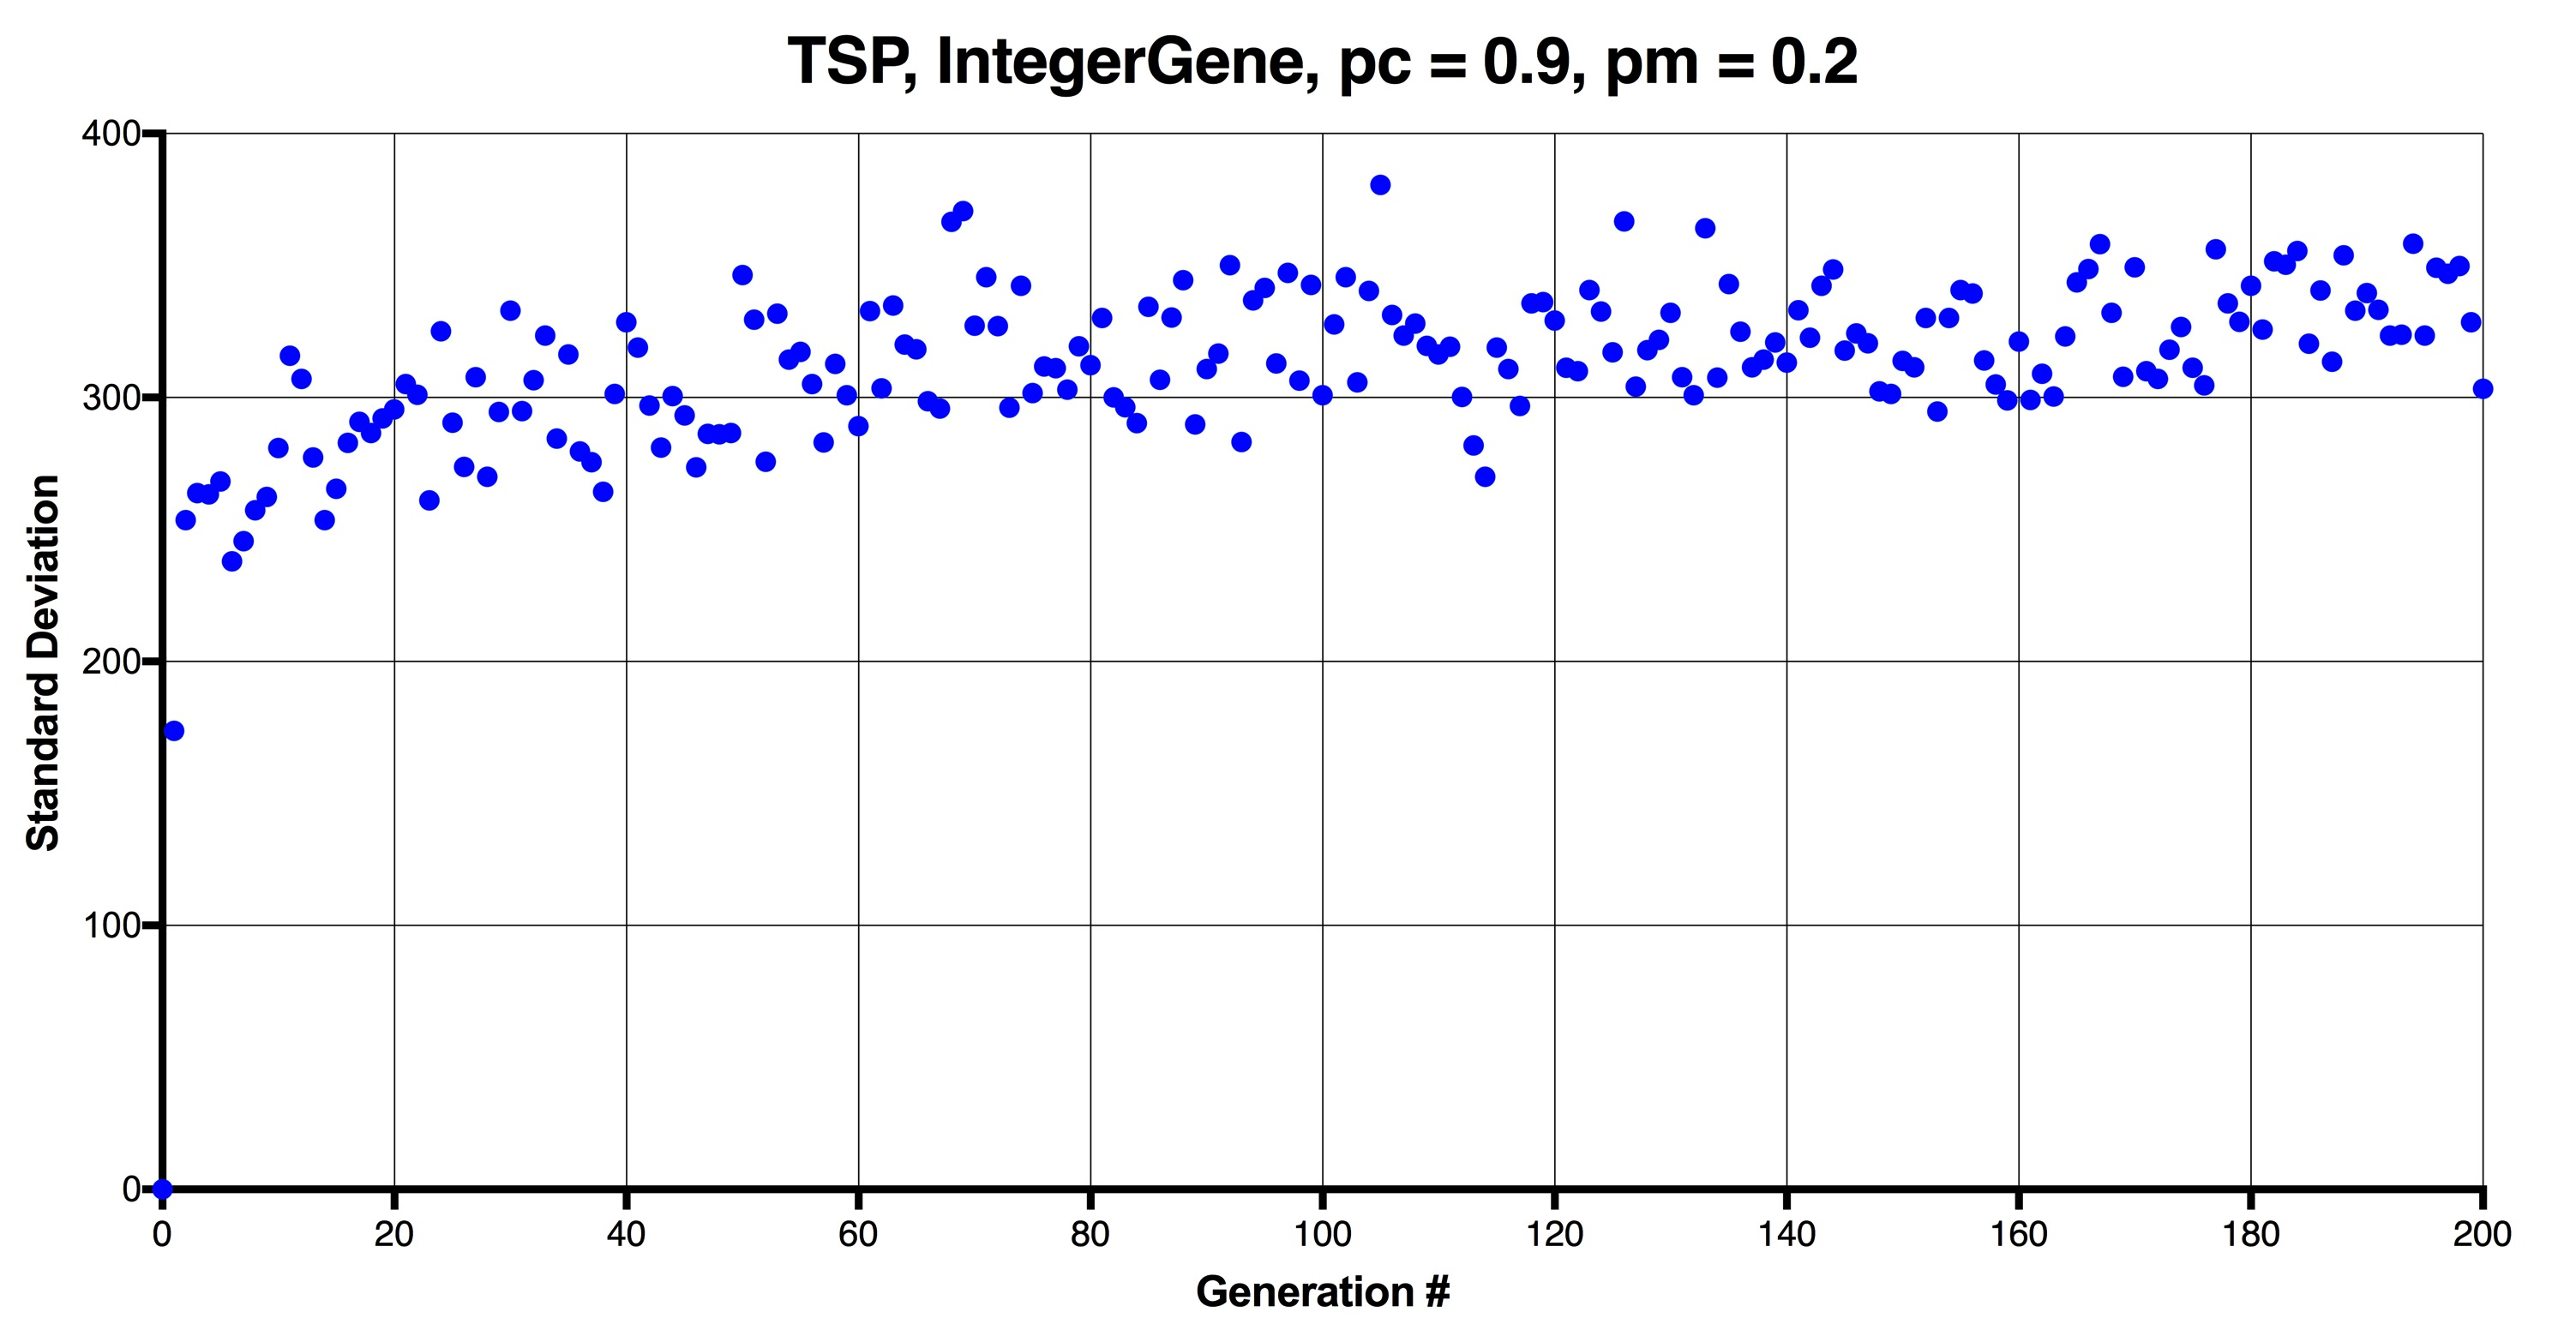
\includegraphics[width=1.0\textwidth]{tsp_02_std.jpg}
    \caption{Desvio padrão ao longo das gerações para o problema do Caixeiro Viajante Adaptado ($p_c=0.9$, ${p_m}_0=0.2$).}
    \label{fig:tsp02std}
\end{figure}

\subsection{Caso Adaptativo ($p_m = 0.01$)}

O caso adaptativo para $p_m = 0.01$ mostrou uma evolução bem diferente do caso estático. Como visto na figura \ref{fig:tsp_001_adaptative}, os indivíduos também conseguiram igualar seus valores de fitness de modo relativamente rápido, mas a melhor solução pôde mudar bem mais rápido. A melhor solução ficou travada por não mais que 76 gerações (região azul entre as gerações 80 e 140), e mesmo assim, os demais indivíduos foram capazes de variar nesse intervalo, o que parece ter ajudado no encontro de soluções melhores. Tal comportamento das soluções pode ser observado nos desvios padrões, mostrados na figura \ref{fig:tsp_001_adaptive_std}.

\begin{figure}[ht!]
    \centering 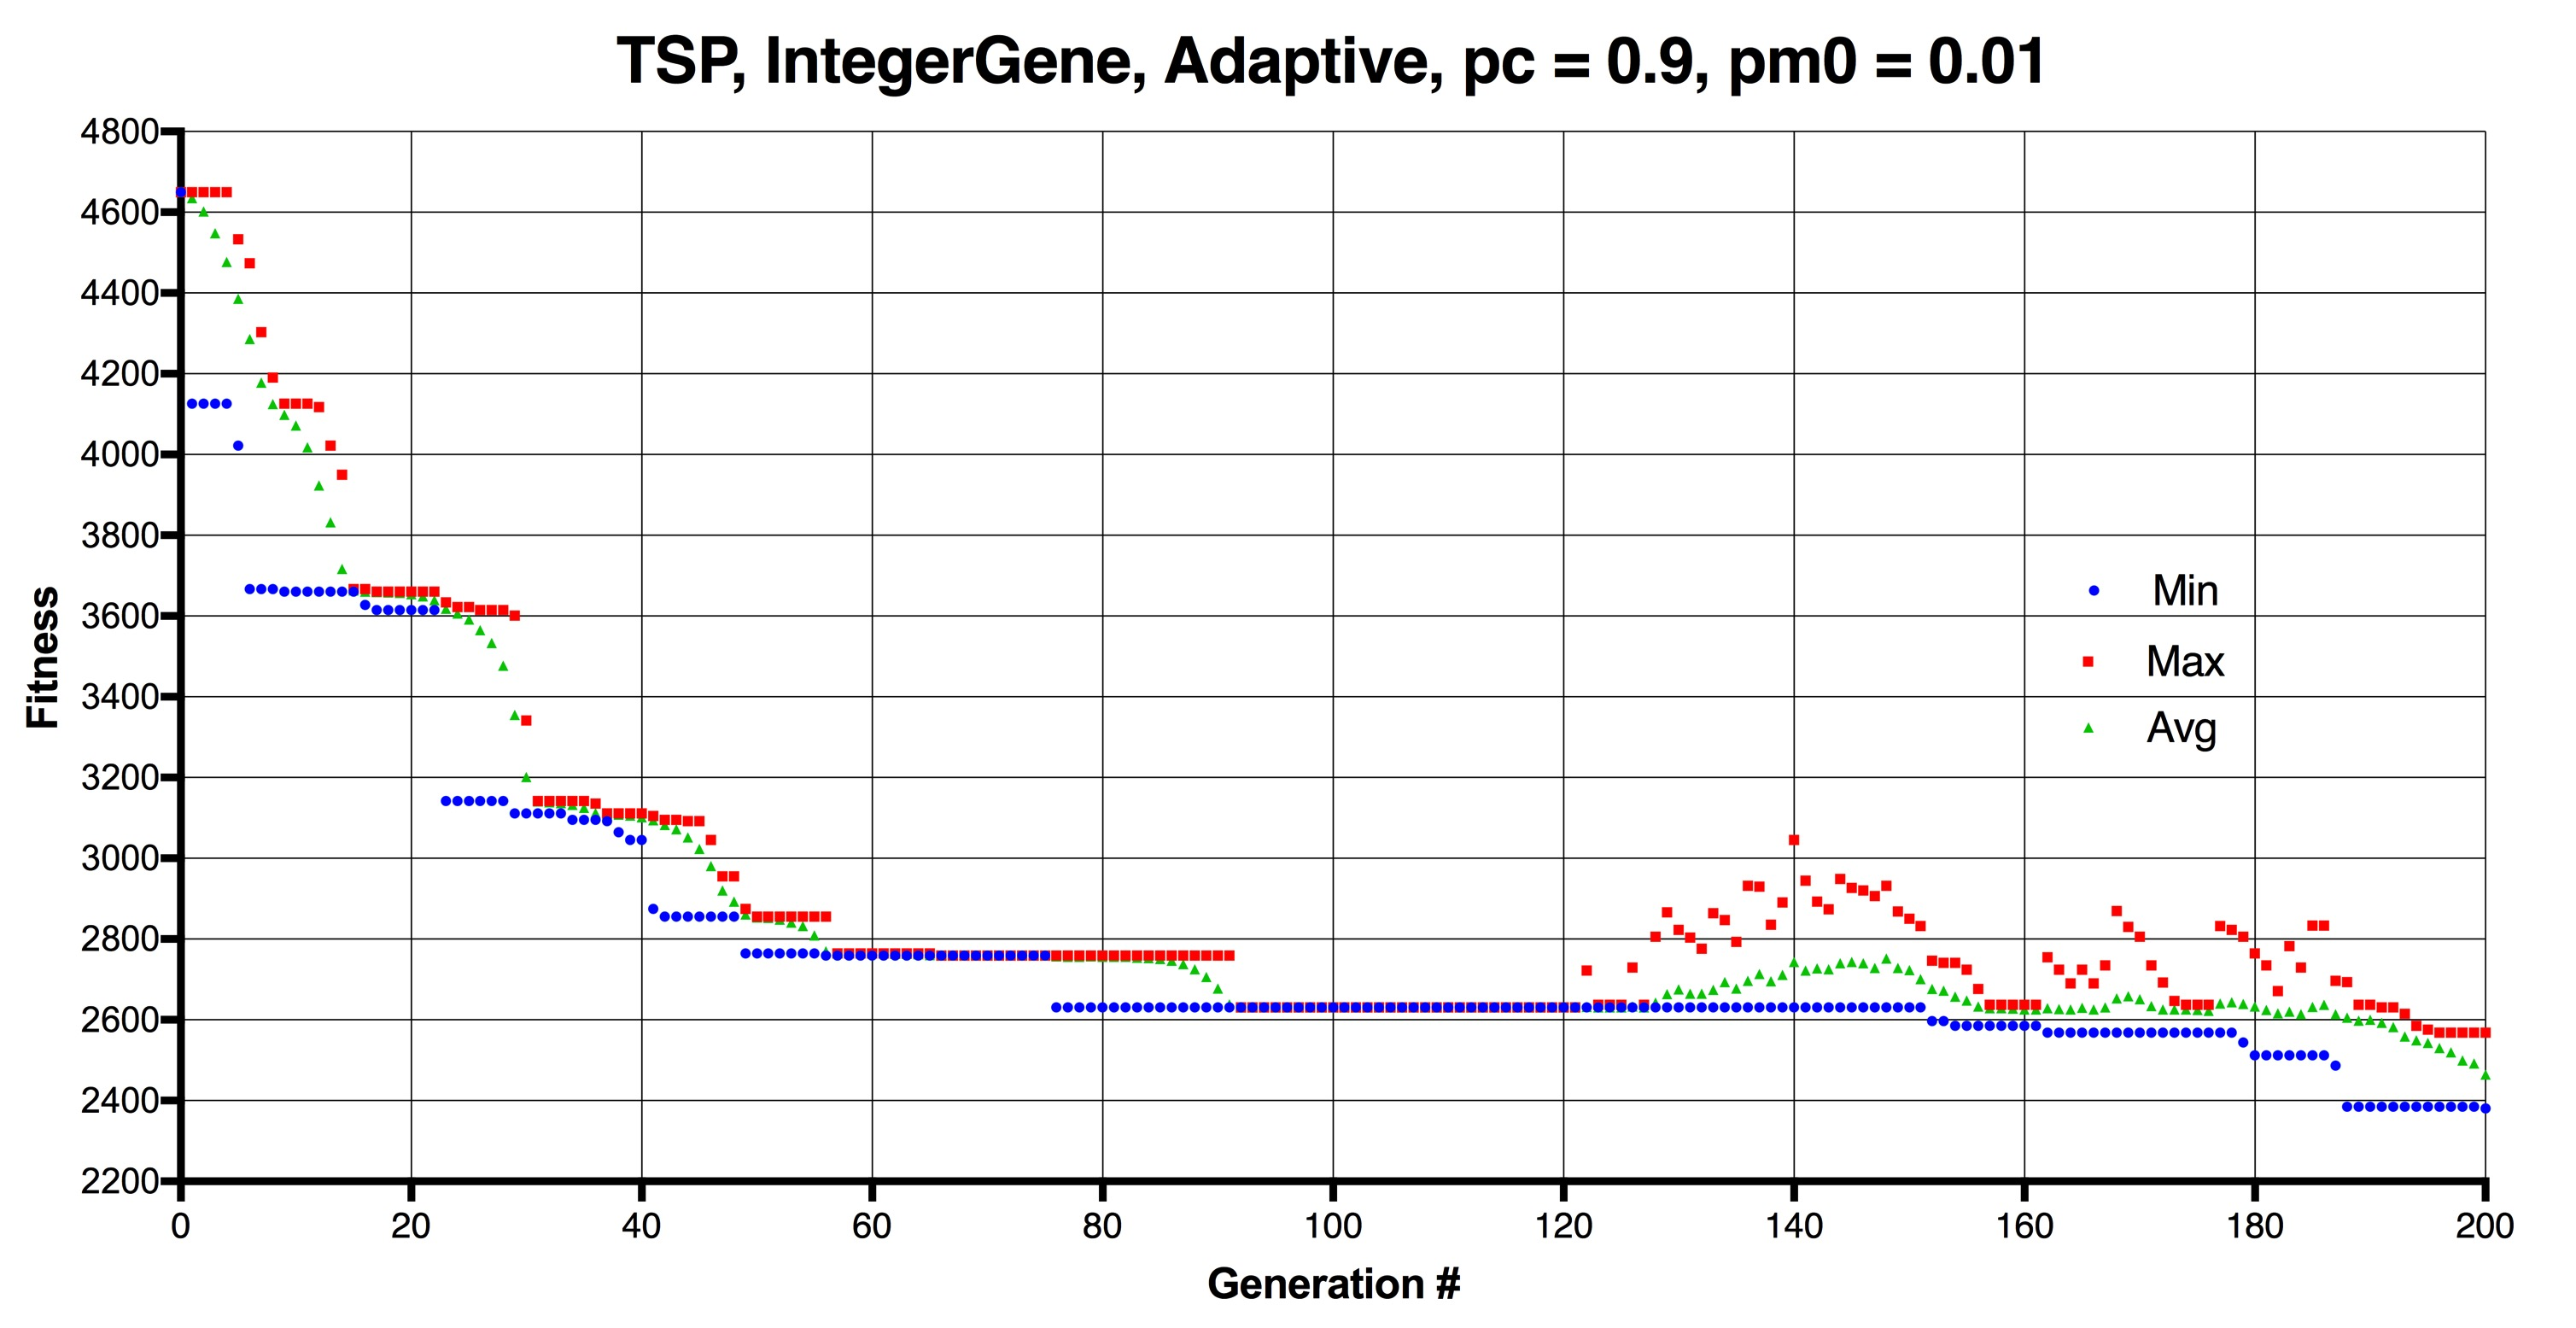
\includegraphics[width=1.0\textwidth]{tsp_001_adaptive.jpg}
    \caption{Evolução do fitness para o problema do Caixeiro Viajante Adaptado Adaptativo, mostrando mínimo, máximo e valor médio ($p_c=0.9$, ${p_m}_0=0.01$). O menor caminho encontrado tem distância total de 2381.}
    \label{fig:tsp_001_adaptative}
\end{figure}

\begin{figure}[ht!]
    \centering 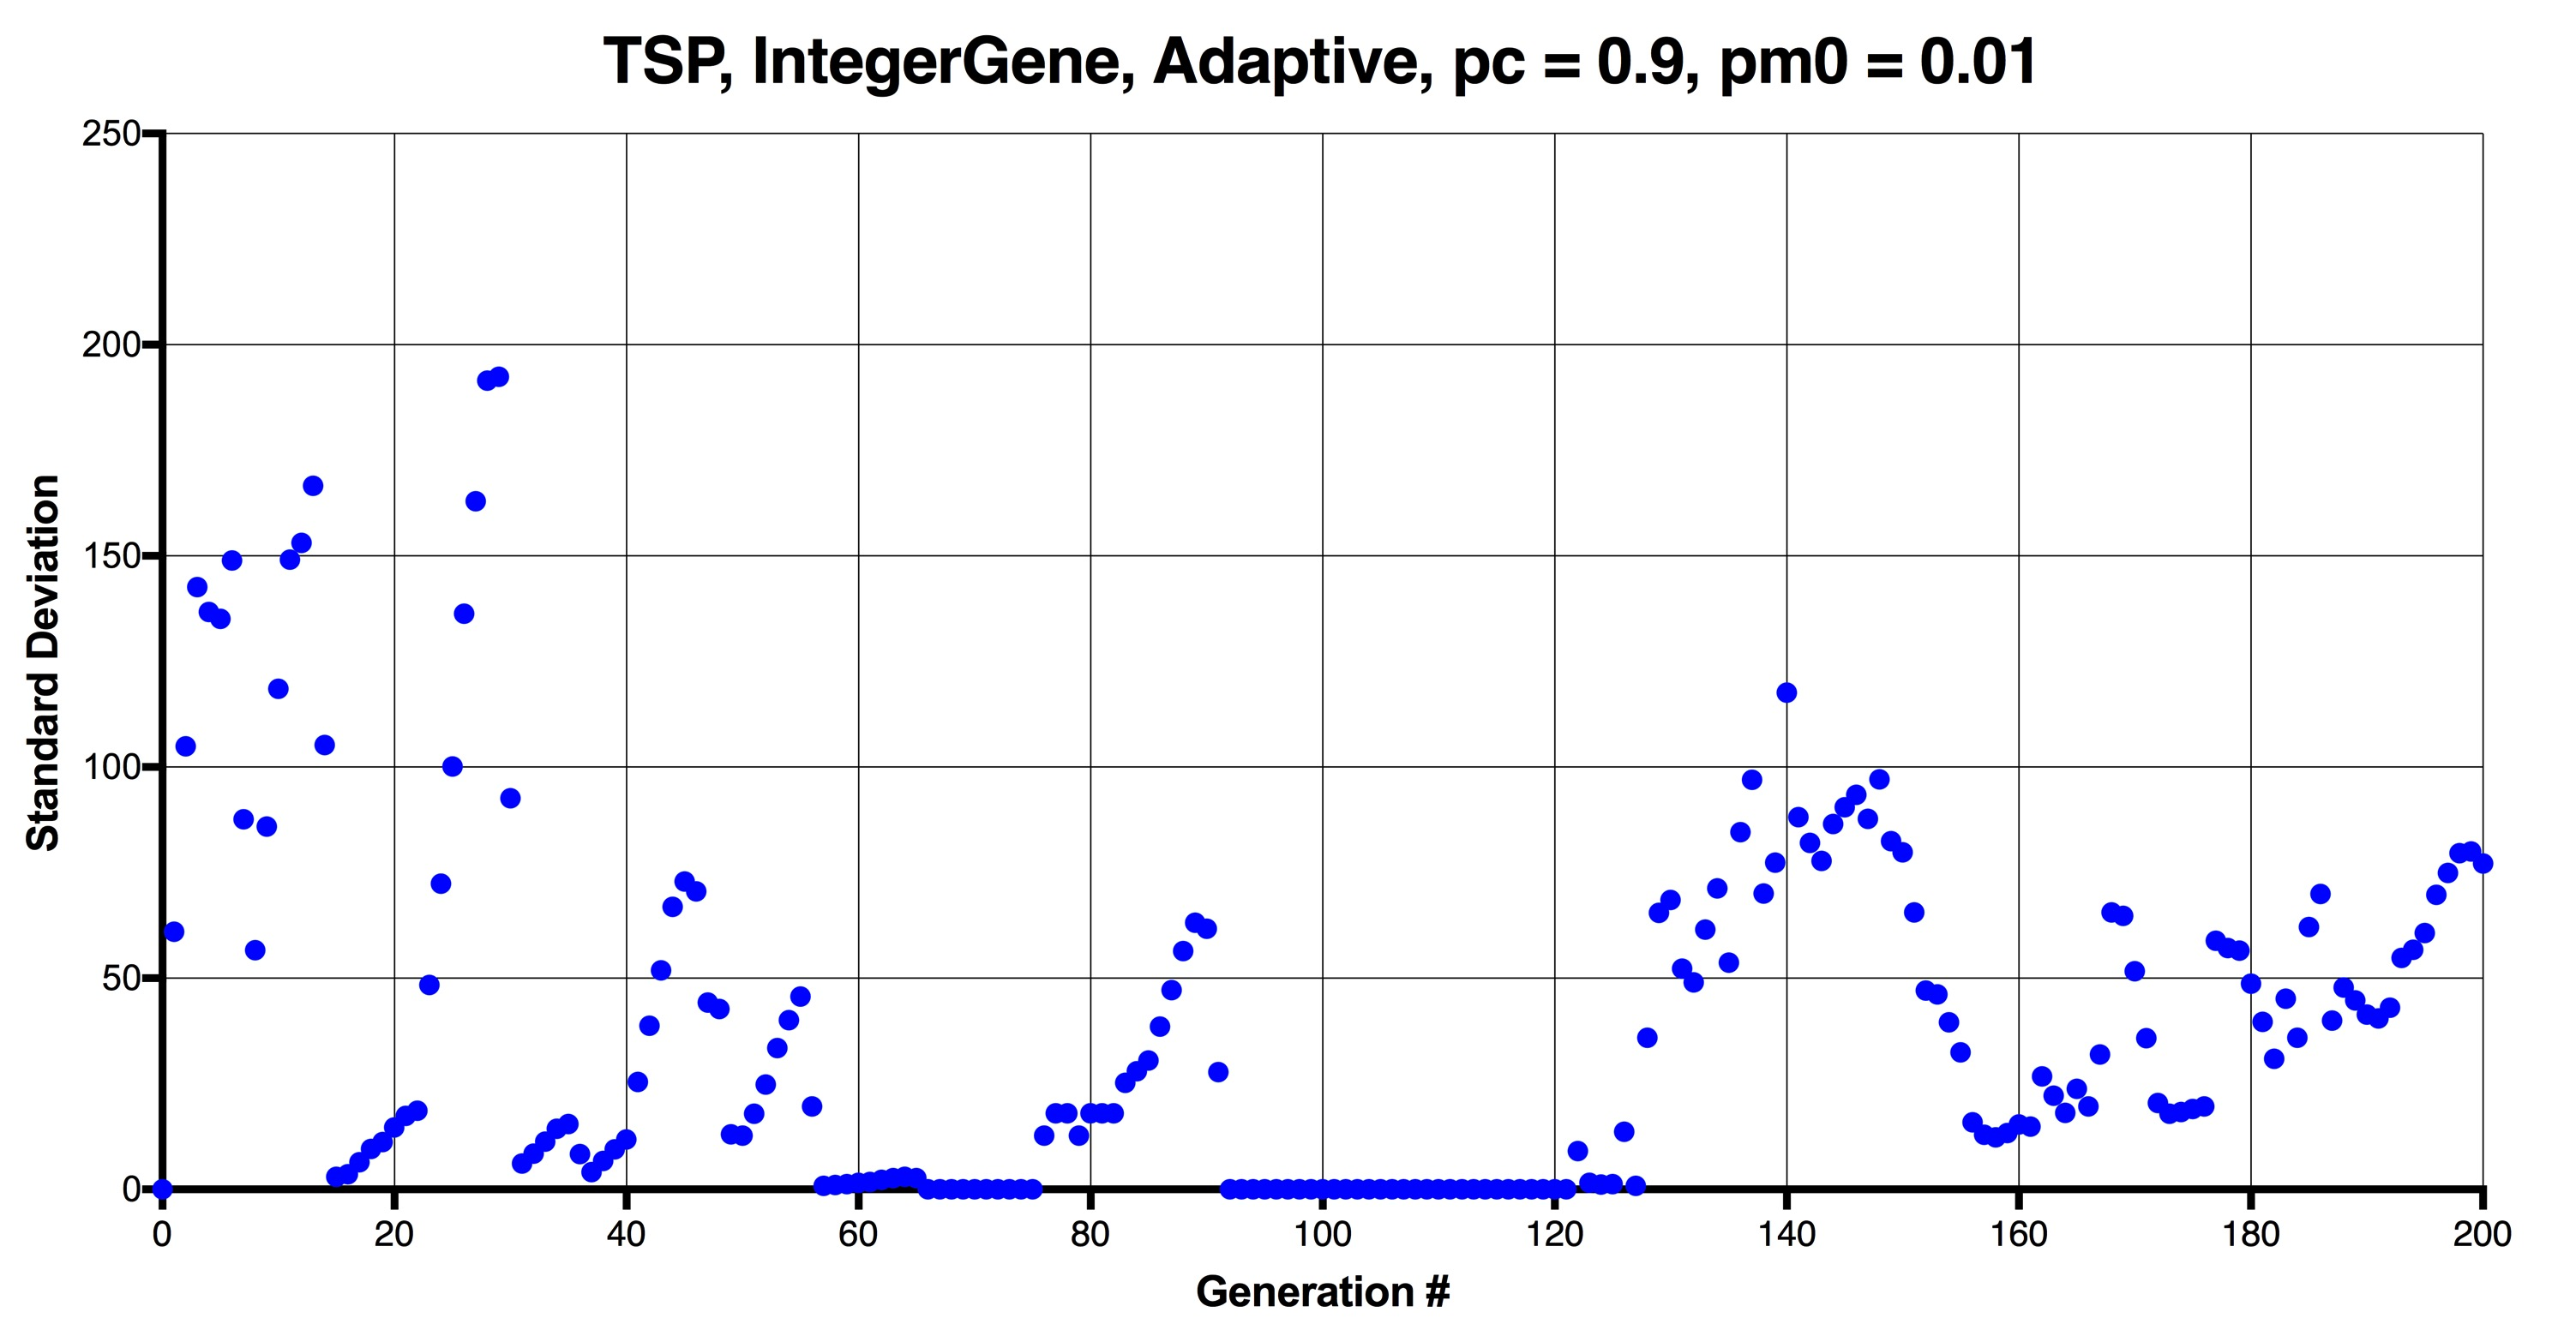
\includegraphics[width=1.0\textwidth]{tsp_001_adaptive_std.jpg}
    \caption{Desvio padrão ao longo das gerações para o problema do Caixeiro Viajante Adaptado Adaptativo ($p_c=0.9$, ${p_m}_0=0.01$).}
    \label{fig:tsp_001_adaptive_std}
\end{figure}

O funcionamento do AGA ficou bem mais evidente na figura \ref{fig:tsp_001_adaptive_pm}, com momentos de aumento e de redução de $p_m$ alternados com maior frequência. Fora isso, ${p_m}_0$ convergiu para um valor bem menor no final da execução (0.024). No entanto, ao contrário dos problemas OneMax, $p_m$ oscilou bastante também ao final das 200 gerações. Isso nos leva a crer que $0.01$ talvez não seja o melhor valor para inicializar ${p_m}_0$. Similar ao caso estático, simulou-se também ${p_m}_0 = 0.2$.

\begin{figure}[ht!]
    \centering 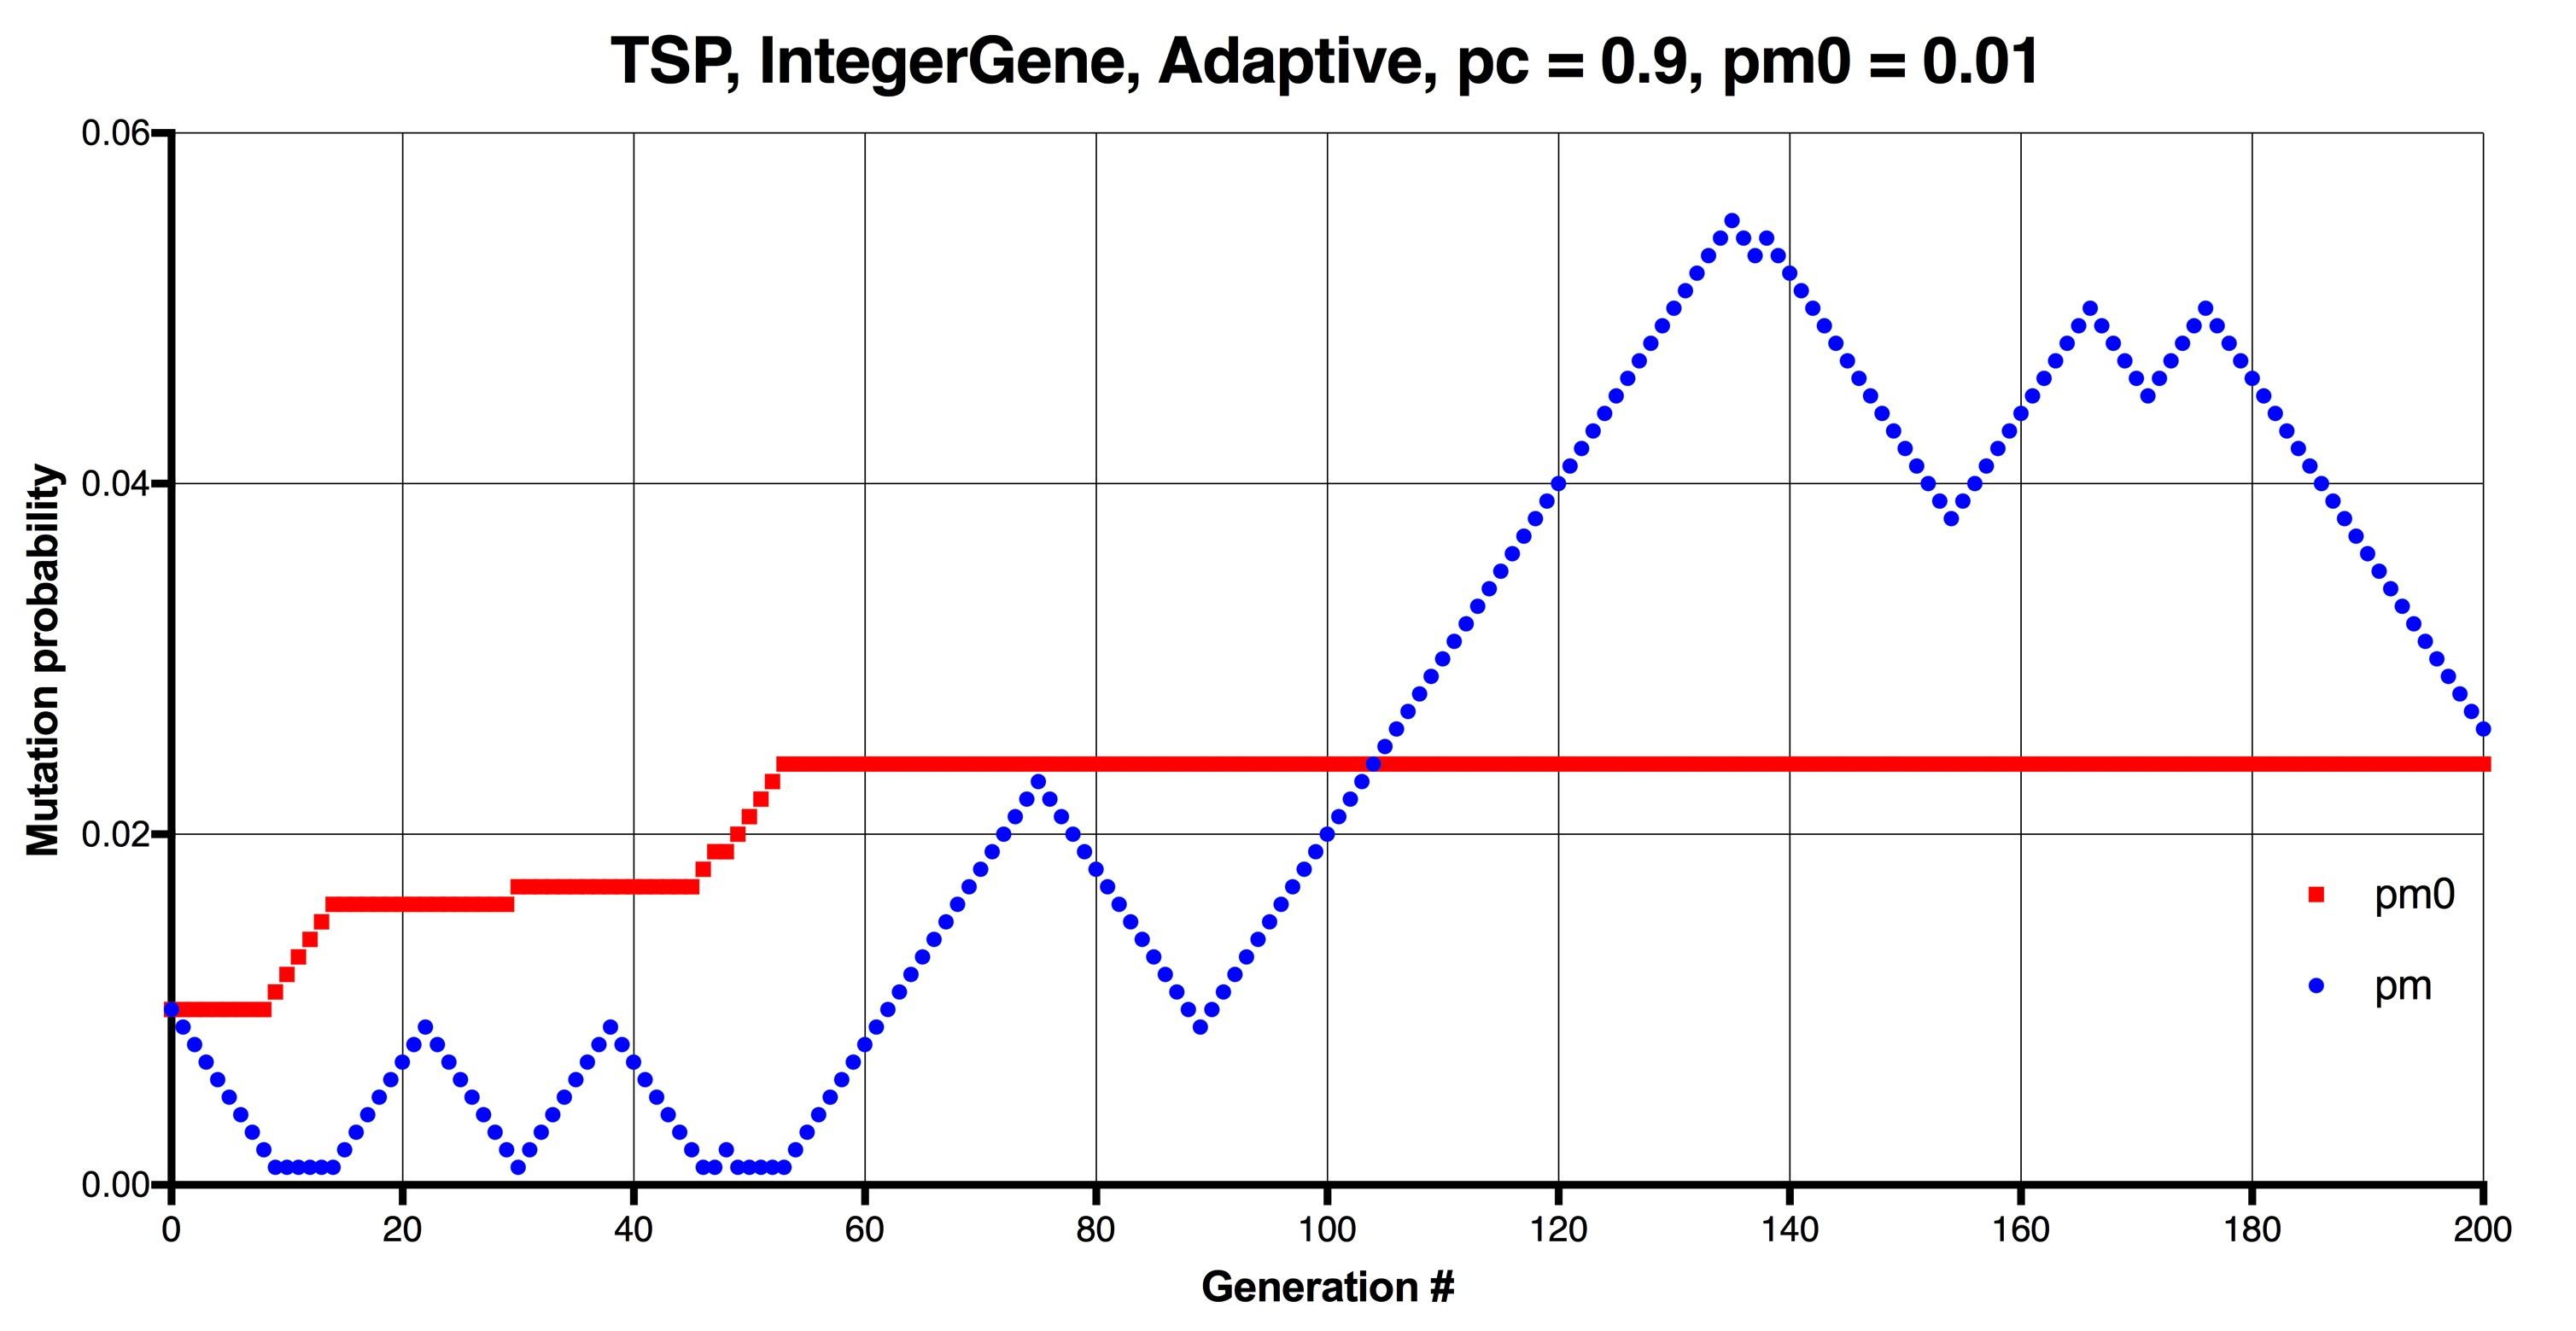
\includegraphics[width=1.0\textwidth]{tsp_001_adaptive_pm.jpg}
    \caption{Probabilidade de mutação ao longo das gerações para o problema do Caixeiro Viajante Adaptado Adaptativo ($p_c=0.9$, ${p_m}_0=0.01$).}
    \label{fig:tsp_001_adaptive_pm}
\end{figure}

\subsection{Caso Adaptativo ($p_m = 0.2$)}

O gráfico da figura \ref{fig:tsp_02_adaptative} encontrou o menor percurso dentre as simulações feitas aqui (2160). Não só isso, as melhores soluções pareceram ficar travadas por bem menos tempo (o pior caso, próximo do final da simulação, durou 34 gerações). Um outro efeito interessante também aconteceu: todas as curvas (mínimo, máximo e média) evoluíram de formas semelhantes, mesmo com uma mutação inicial intensa. Isso deu para observar também na evolução do desvio padrão, na figura \ref{fig:tsp_02_adaptive_std}, que conseguiu diminuir com o tempo e ficar mais ou menos estável ao longo das gerações.

\begin{figure}[ht!]
    \centering 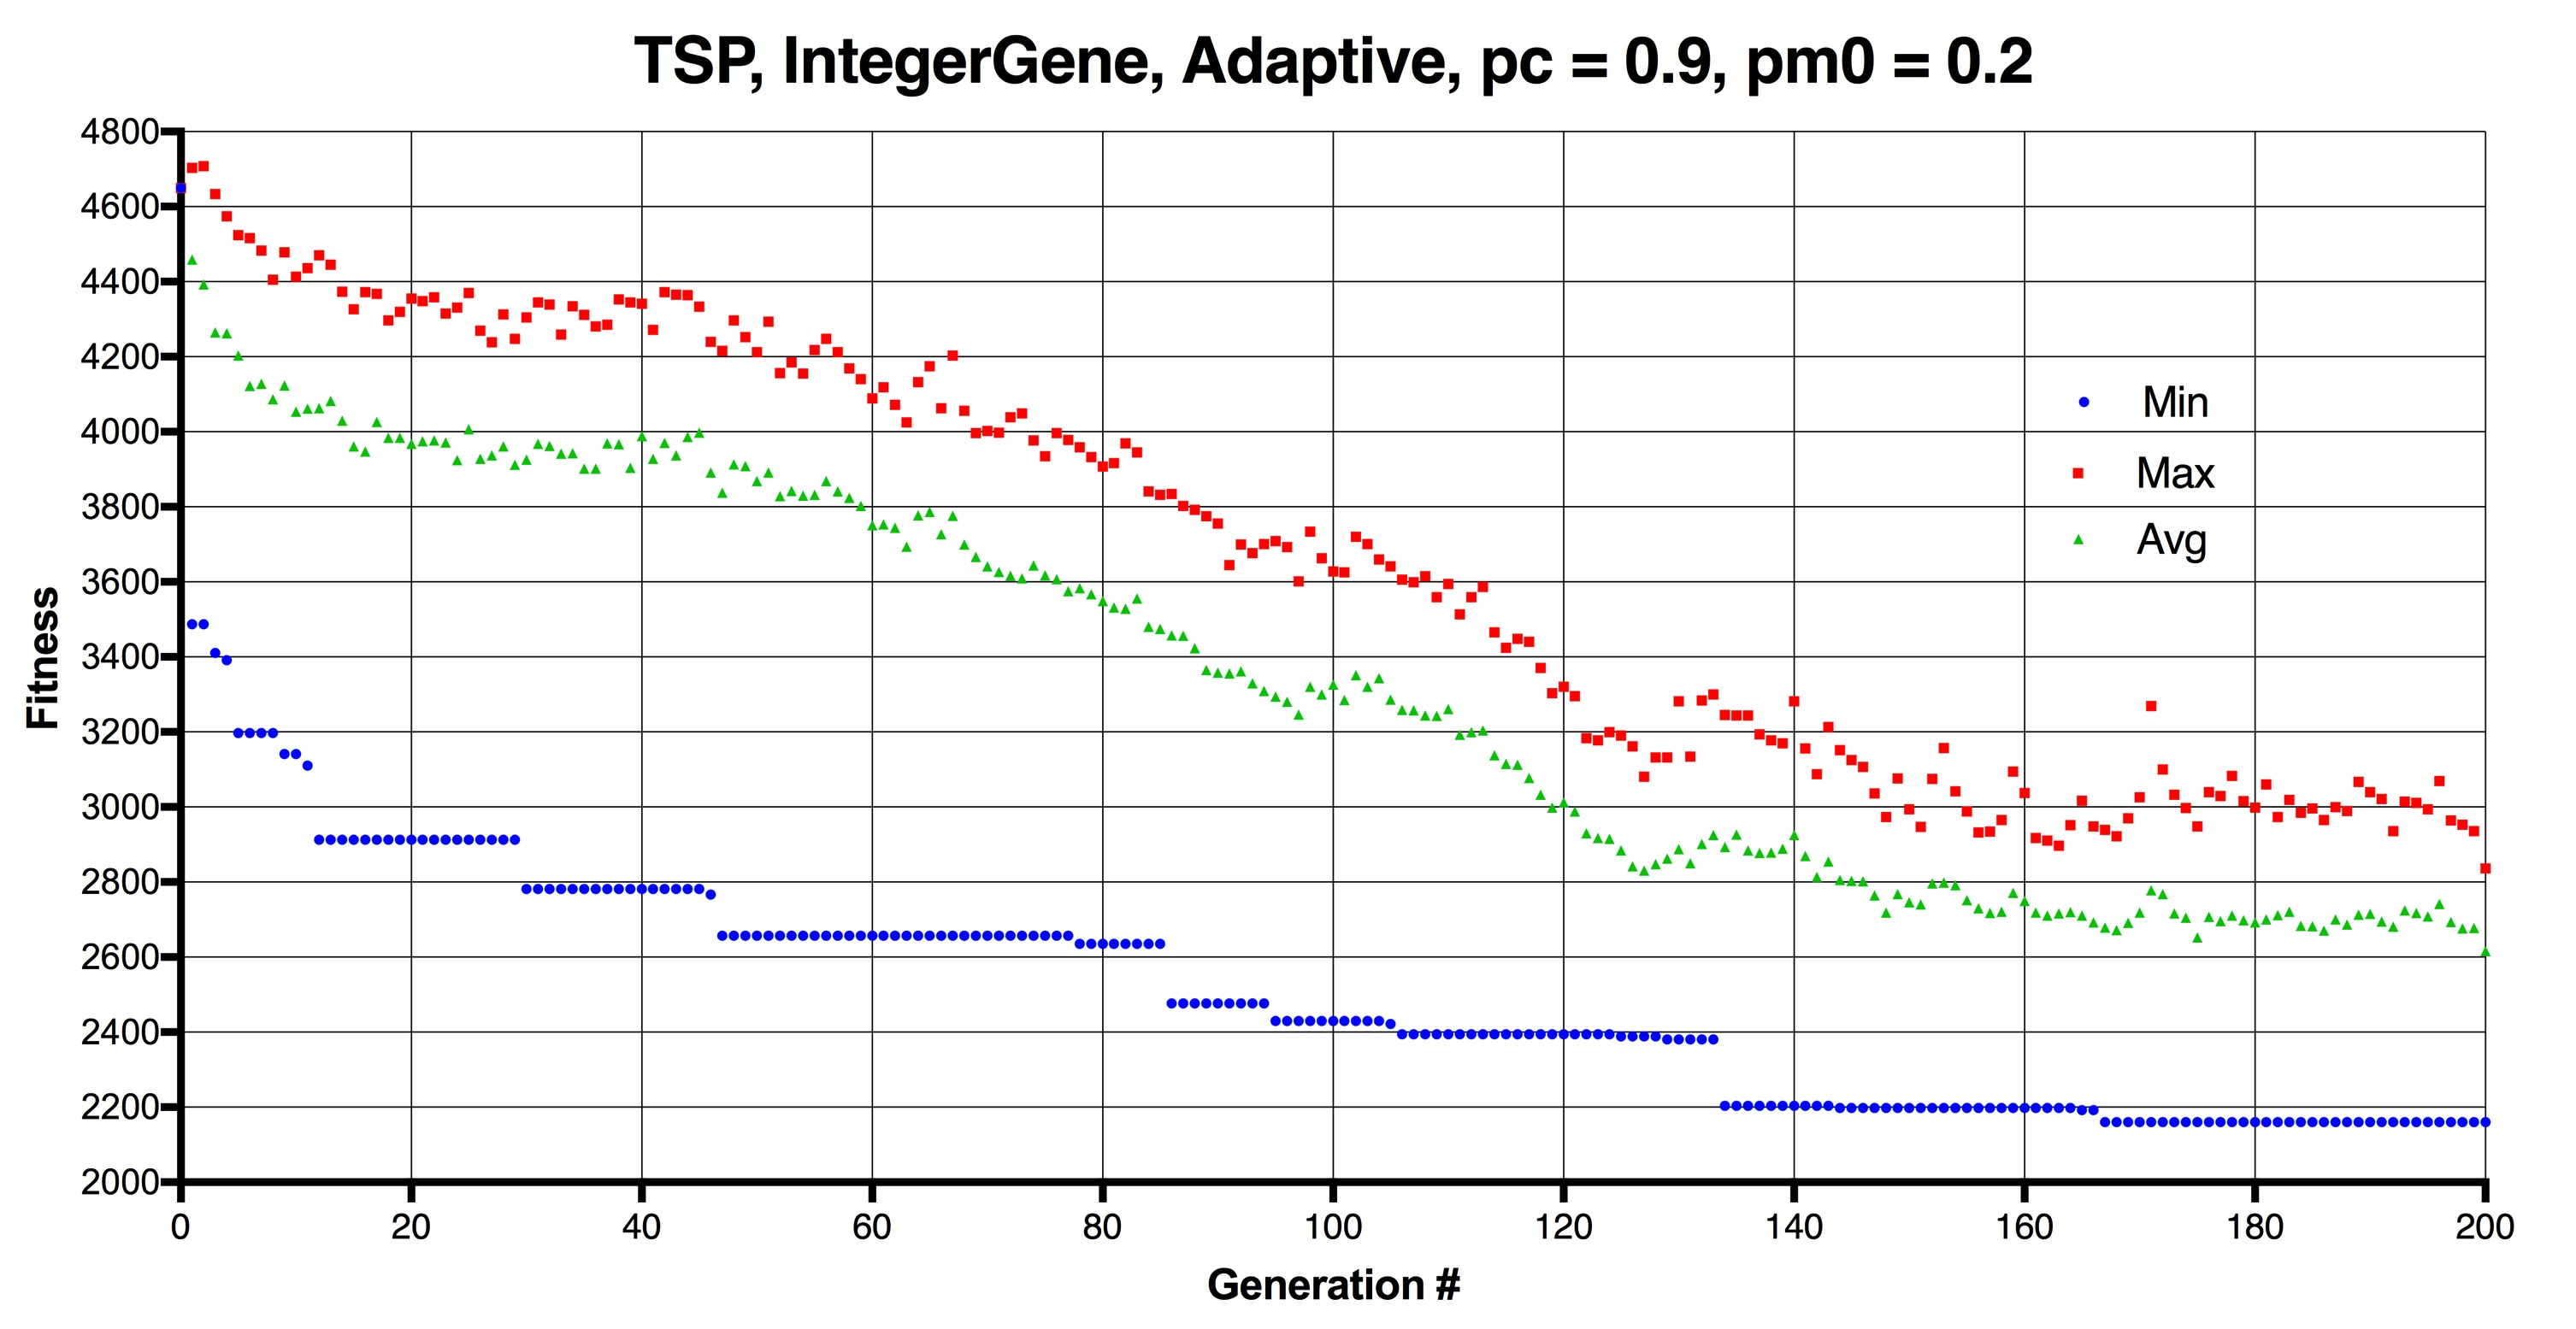
\includegraphics[width=1.0\textwidth]{tsp_02_adaptive.jpg}
    \caption{Evolução do fitness para o problema do Caixeiro Viajante Adaptado Adaptativo, mostrando mínimo, máximo e valor médio ($p_c=0.9$, ${p_m}_0=0.2$). O menor caminho encontrado tem distância total de 2160.}
    \label{fig:tsp_02_adaptative}
\end{figure}

\begin{figure}[ht!]
    \centering 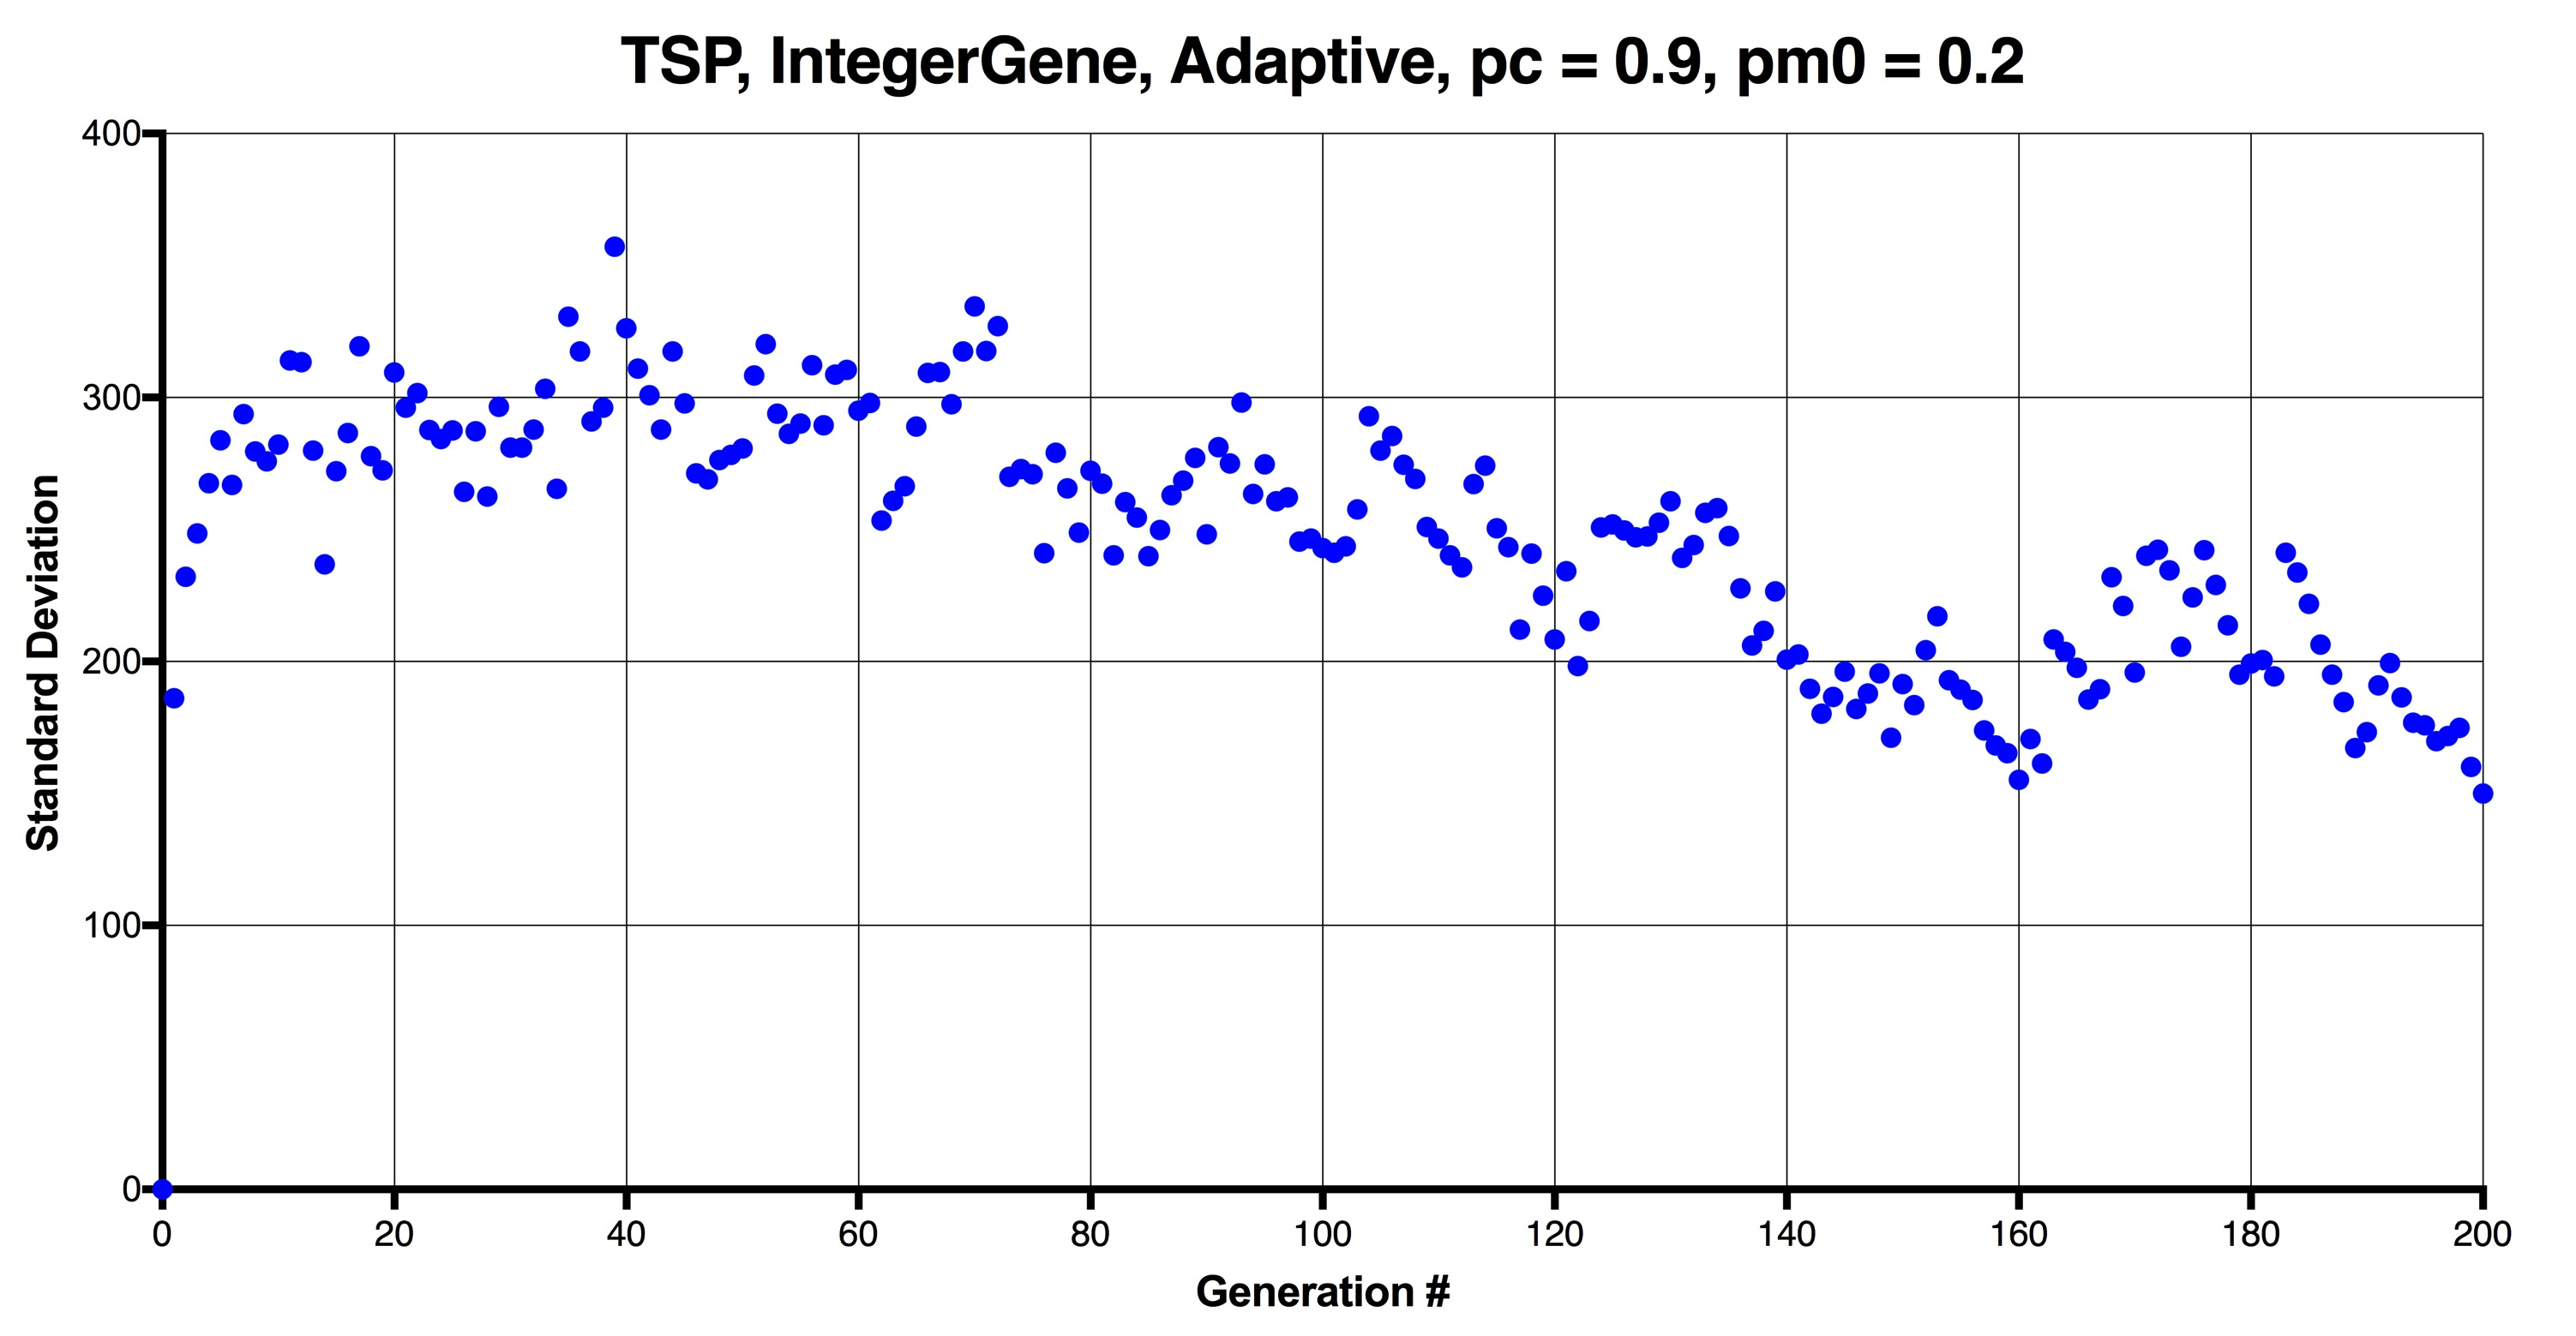
\includegraphics[width=1.0\textwidth]{tsp_02_adaptive_std.jpg}
    \caption{Desvio padrão ao longo das gerações para o problema do Caixeiro Viajante Adaptado Adaptativo ($p_c=0.9$, ${p_m}_0=0.2$).}
    \label{fig:tsp_02_adaptive_std}
\end{figure}

A curva de interesse aqui foi certamente a da figura \ref{fig:tsp_02_adaptive_pm}. O valor de ${p_m}_0$ não mudou em momento algum, e $p_m$ se estabilizou entorno de seu valor final (0.084). Esta é a curva que melhor demonstra o potencial do AGA desenvolvido aqui: mesmo começando num valor desfavorável para convergência, $p_m$ mudou de patamar e foi estabilizado, trazendo a melhor resposta e a melhor evolução para este problema em 200 gerações.

\begin{figure}[ht!]
    \centering 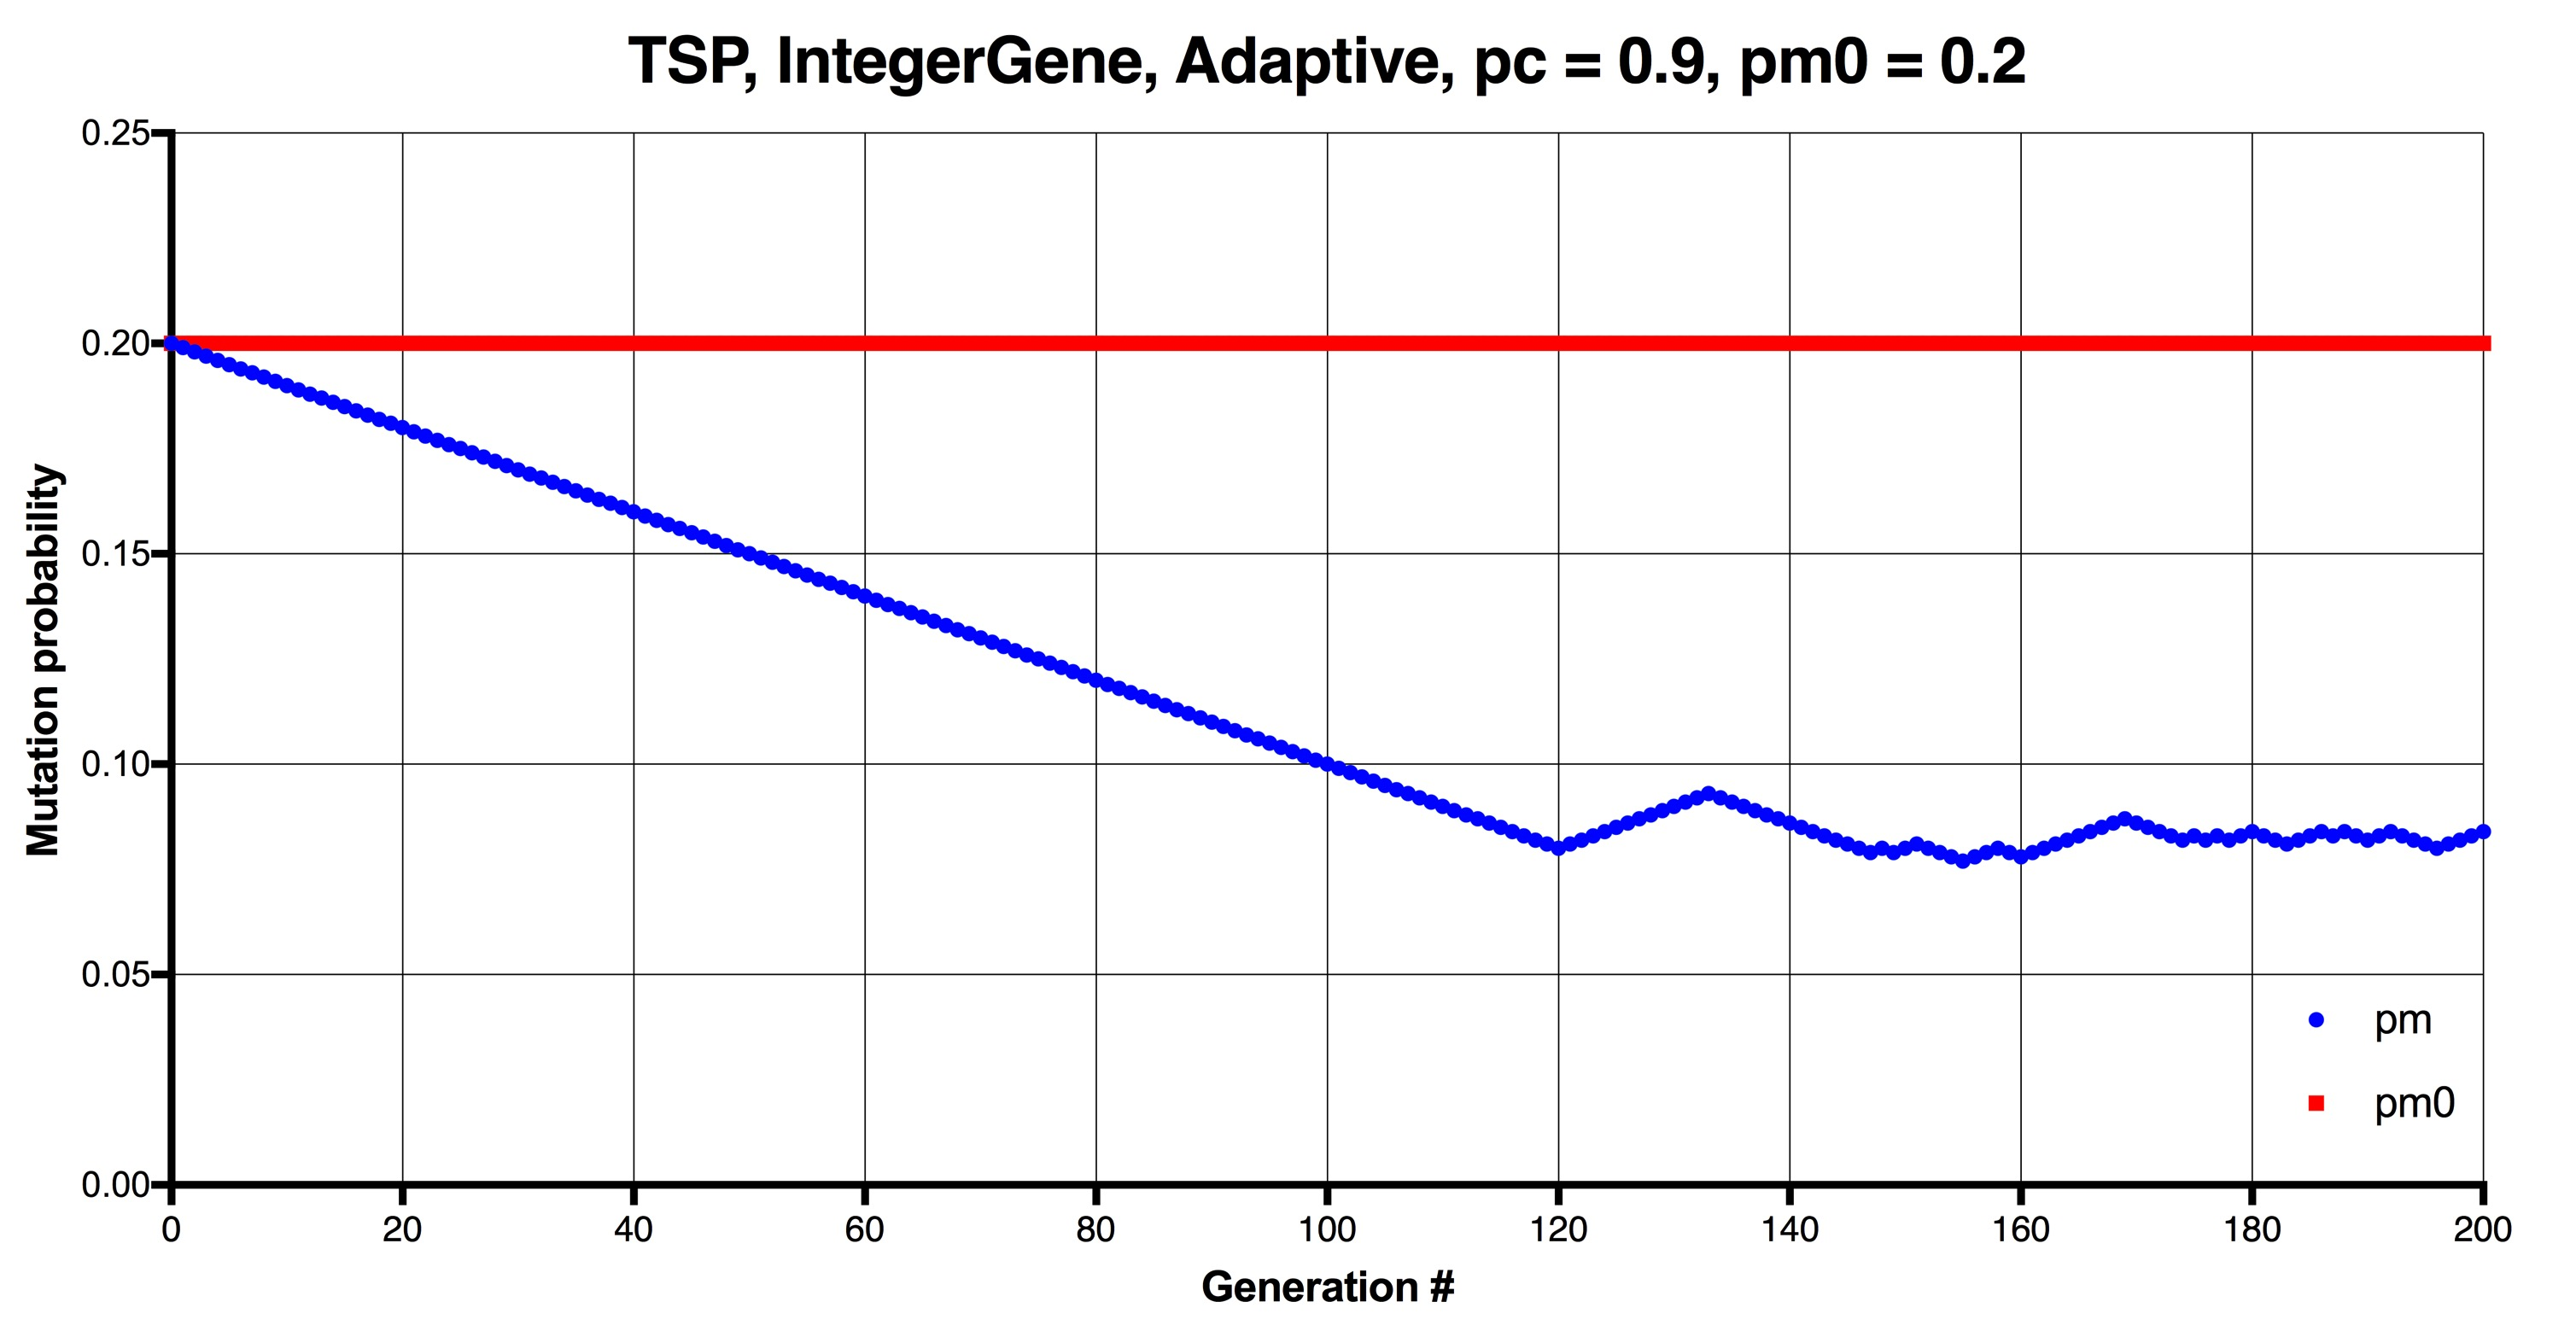
\includegraphics[width=1.0\textwidth]{tsp_02_adaptive_pm.jpg}
    \caption{Probabilidade de mutação ao longo das gerações para o problema do Caixeiro Viajante Adaptado Adaptativo ($p_c=0.9$, ${p_m}_0=0.2$).}
    \label{fig:tsp_02_adaptive_pm}
\end{figure}

Os dados de interesse destas quatro simulações estão presentes na tabela \ref{tab:tsp}.

\begin{table}
\caption{Dados coletados do problema do Caixeiro Viajante Adaptado.}
\label{tab:tsp}

\centering
\begin{tabular}[!hbt]{|c|cc|cc|}
	\hline
	Valor inicial de $p_m$								& \multicolumn{2}{c|}{0.01}		& \multicolumn{2}{c|}{0.2}	\\
	\hline
	Algoritmo analisado (AG = caso estático)			& AG		& AGA		& AG		& AGA		\\
	\hline
	Fitness mínimo após 100 gerações					& $2631$	& $2631$	& $2418$	& $2430$	\\
	Fitness médio após 100 gerações						& $2631$	& $2631$	& $3819.5$	& $3325.88$	\\
	Fitness mínimo após 200 gerações 					& $2375$	& $2381$	& $2300$	& $2160$	\\
	Fitness médio após 200 gerações 					& $2375$	& $2464.54$	& $3948.11$	& $2615.89$	\\
	\# máximo de gerações "travado" num mínimo local	& $118$		& $76$		& $127$		& $34$		\\
	Valor final de $p_m$								& $0.01$	& $0.026$	& $0.2$		& $0.084$	\\
	Valor mínimo de $p_m$								& $0.01$	& $0.001$	& $0.2$		& $0.077$	\\
	Valor máximo de $p_m$								& $0.01$	& $0.055$	& $0.2$		& $0.2$		\\
	Valor médio de $p_m$								& $0.01$	& $0.0249$	& $0.2$		& $0.117$	\\
	Valor médio de $p_m$ (últimas 100 gerações)			& $0.01$	& $0.0413$	& $0.2$		& $0.0846$	\\
	Valor final de ${p_m}_0$							& --		& $0.024$	& --		& $0.2$		\\
	\hline
\end{tabular}
\end{table}

\section{Discussões}

Os três problemas foram simulados tanto pelo AG estático quanto pelo AGA. Para os problemas OneMax, foi possível observar uma evolução muito melhor para o caso estático do que para o caso adaptativo. Para o problema do Caixeiro Viajante Adaptado, no entanto, observou-se o oposto. Seria possível validar o AGA a partir destes experimentos?

Pensemos nas operações de variação de um AG. Se associarmos probabilidade de crossover $p_c$ (alta) ao fator de homogeneização do fitness da população, então a probabilidade de mutação $p_m$, combinada com elitismo, pode atuar de duas formas:

\begin{itemize}
	\item Tornando a população heterogênea;
	\item \textbf{Melhorando o fitness do melhor indivíduo}.
\end{itemize}

O efeito que será mais predominante dependerá do valor de $p_m$ e do problema. Como visto no OneMax, um valor de 0.01 ou de 0.001 foi suficiente para priorizar o segundo efeito sobre o primeiro, evoluindo gradualmente o melhor indivíduo.

No entanto, o problema do Caixeiro Viajante Adaptado não conseguiu se beneficiar destes efeitos nem para $p_m=0.01$, nem para $p_m=0.2$. Não que o AG estático não possua um valor ideal para convergência deste problema em específico - isto apenas atesta que o parâmetro ideal para um problema pode não ser ideal para outro problema.

Se tentássemos estressar o problema do Caixeiro, poderíamos eventualmente encontrar um valor ideal para ${p_m}_0$. No entanto, tal problema (mesmo adaptado) ainda é NP-Hard, e um valor estático de $p_m$ pode não ser suficiente para encontrar o mínimo global. O que resolveria este problema, quando um valor muito baixo e um valor muito alto de ${p_m}_0$ não são suficientes?

Tal questionamento trouxe a este trabalho a ideia de se usar um algoritmo adaptativo. Algo a se acrescentar ao AG que permitisse adaptar o valor de $p_m$ ao longo das gerações. Mesmo que o uso do AGA não trouxesse melhores soluções mais rapidamente, ele se mostrou melhor para o encontro de percursos cada vez menores. No entanto, o uso do AGA não trouxe o mesmo benefício para os problemas OneMax. Repensar o AGA é uma ideia válida, mas usar o AGA será sempre uma ideia melhor?

Para isso, é necessário considerar os teoremas "No Free Lunch" (NFL - em português, teriam a mesma origem da expressão "Não existe almoço grátis") \cite{wolpert1997no}. De maneira simples, estes teoremas dizem que, para um algoritmo de busca e otimização (como é o caso do AG e do AGA), uma performance elevada para um grupo de problemas (como os problemas OneMax) tem como preço uma queda de performance para todos os outros grupos de problemas (como o problema do Caixeiro Viajante). O AGA tentaria ser a adaptação do AG para se adequar a outros problemas, e mesmo assim, ele veio com uma perda de performance para os problemas OneMax.

Não é possível utilizar o mesmo algoritmo para todos os problemas. Mesmo que não utilizássemos um AGA, ainda haveria formas melhores de se otimizar o AG para um grupo de problemas, incluindo o Caixeiro Viajante. Isso, no entanto, não tira o mérito do AGA.

Pelos experimentos feitos neste trabalho, ele foi capaz de encontrar soluções melhores para um problema mais complexo que os OneMax. Melhor performance é sempre interessante, mas ser capaz de encontrar soluções cada vez melhores sem ficar travado em extremos locais é, ao olhos deste trabalho, um benefício muito melhor. Restaria então verificar se outros problemas conseguiriam se beneficiar do AGA da mesma forma, e se o algoritmo do AGA poderia ser melhorado também.


\chapter{Conclus\oes e Trabalhos Futuros}
\label{6_conclusoes}

\section{Conclusões}

Este trabalho teve como objetivo o desenvolvimento de um Algoritmo Genético (AG) para a resolução de diferentes problemas de modo otimizado. Foram escolhidos três problemas: OneMax Booleano (variável booleana), OneMax Real (variável real) e Caixeiro Viajante Adaptado (permitindo atalhos). De modo a melhorar a performance do AG, foram implementadas duas otimizações: o elitismo do melhor indivíduo, e o uso de um Algoritmo Genético Adaptativo (AGA) com implementação própria, focada na adaptação do parâmetro de mutação.

Chegou-se à conclusão que utilizar um mesmo algoritmo para resolver um grupo diferente de problemas sem perda de performance é virtualmente impossível. No entanto, o uso do AGA implementado se mostrou mais eficiente no encontro de melhores soluções para o problema do Caixeiro Viajante, um problema NP-Hard. Por conta disso, o uso deste AGA é fortemente incentivado em outros problemas, buscando sempre validações e melhorias. Se isso não for possível, o conceito por trás do desenvolvimento de um algoritmo adaptativo é muito forte e próximo do conceito básico do AG, e seu uso deve ser considerado em outros algoritmos evolutivos.

\section{Trabalhos Futuros}

O desenvolvimento feito neste trabalho resultaram na criação de um algoritmo adaptativo e de implementações próprias tanto do algoritmo genético quanto dos problemas escolhidos. A proposta deste trabalho foi audaz, e muitos conceitos foram desenvolvidos ao mesmo tempo, conceitos que precisam ser quebrados e maturados ainda mais. Sugere-se então as seguintes frentes de trabalho futuro:

\begin{itemize}

	\item Análise mais cuidadosa do problema do OneMax Real, considerando modelagens matemáticas e sua proximidade com o OneMax Booleano;

	\item Análise do problema do Caixeiro Viajante com a distribuição genética deste trabalho, comparada com implementações mais tradicionais (este trabalho distribuiu os genes deste problema de tal forma que o crossover de dois pontos ainda fosse possível);

	\item Evolução dos conceitos por trás do AGA desenvolvido aqui, buscando formalizar os conceitos por trás de seu desenvolvimento e, onde for possível, melhorá-lo (tanto para performance quanto para busca de soluções);

	\item Testar o AGA junto a outros problemas, para verificar prós, contras e limitações;

	\item Os gráficos de teste do AGA mostraram um comportamento aproximadamente periódico para a curva de $p_m$ e do desvio, mesmo com o comportamento aleatório da mutação. Pode ser interessante estudar este comportamento;

	\item O algoritmo em si foi pouco trabalhado (mesmo tendo muita coisa sendo discutida aqui), dado o tempo utilizado para este trabalho. Recomenda-se uma melhoria drástica deste algoritmo de modo a comportar outras implementações dos problemas, dos operadores de evolução e de outros algoritmos adaptativos.

\end{itemize}


\bibliography{referencias}
\bibliographystyle{plain}

\appendix

\newpage
\chapter{Genes Utilizados}
\label{appendix:genes}
\lstinputlisting[language={python}, caption={Genes Utilizados (genes.py).}]{\src/genes.py}

\newpage
\chapter{Indivíduos dos problemas}
\label{appendix:genes}
\lstinputlisting[language={python}, caption={Indivíduos dos problemas (individuals.py).}]{\src/individuals.py}

\newpage
\chapter{Algoritmo Genético}
\label{appendix:geneflow}
\lstinputlisting[language={python}, caption={Algoritmo Genético (geneflow.py).}]{\src/geneflow.py}

\newpage
\chapter{Funções de fitness}
\label{appendix:fitness}
\lstinputlisting[language={python}, caption={Funções de fitness (fitness.py).}]{\src/fitness.py}

\newpage
\chapter{Mapa das cidades - Caixeiro Viajante}
\label{appendix:dijks}
\lstinputlisting[language={python}, caption={Arquivo com mapa das cidades - Caixeiro Viajante (dijkstra17.py).}]{\src/dijkstra17.py}

\newpage
\chapter{Implementação do Algoritmo de Dijkstra}
\label{appendix:dijks}
\lstinputlisting[language={python}, caption={Arquivo com algoritmo de Dijkstra (dijkstra.py).}]{\src/dijkstra.py}

\newpage
\chapter{Funções de utilidade}
\label{appendix:fitness}
\lstinputlisting[language={python}, caption={Funções de utilidade (utils.py)}]{\src/utils.py}

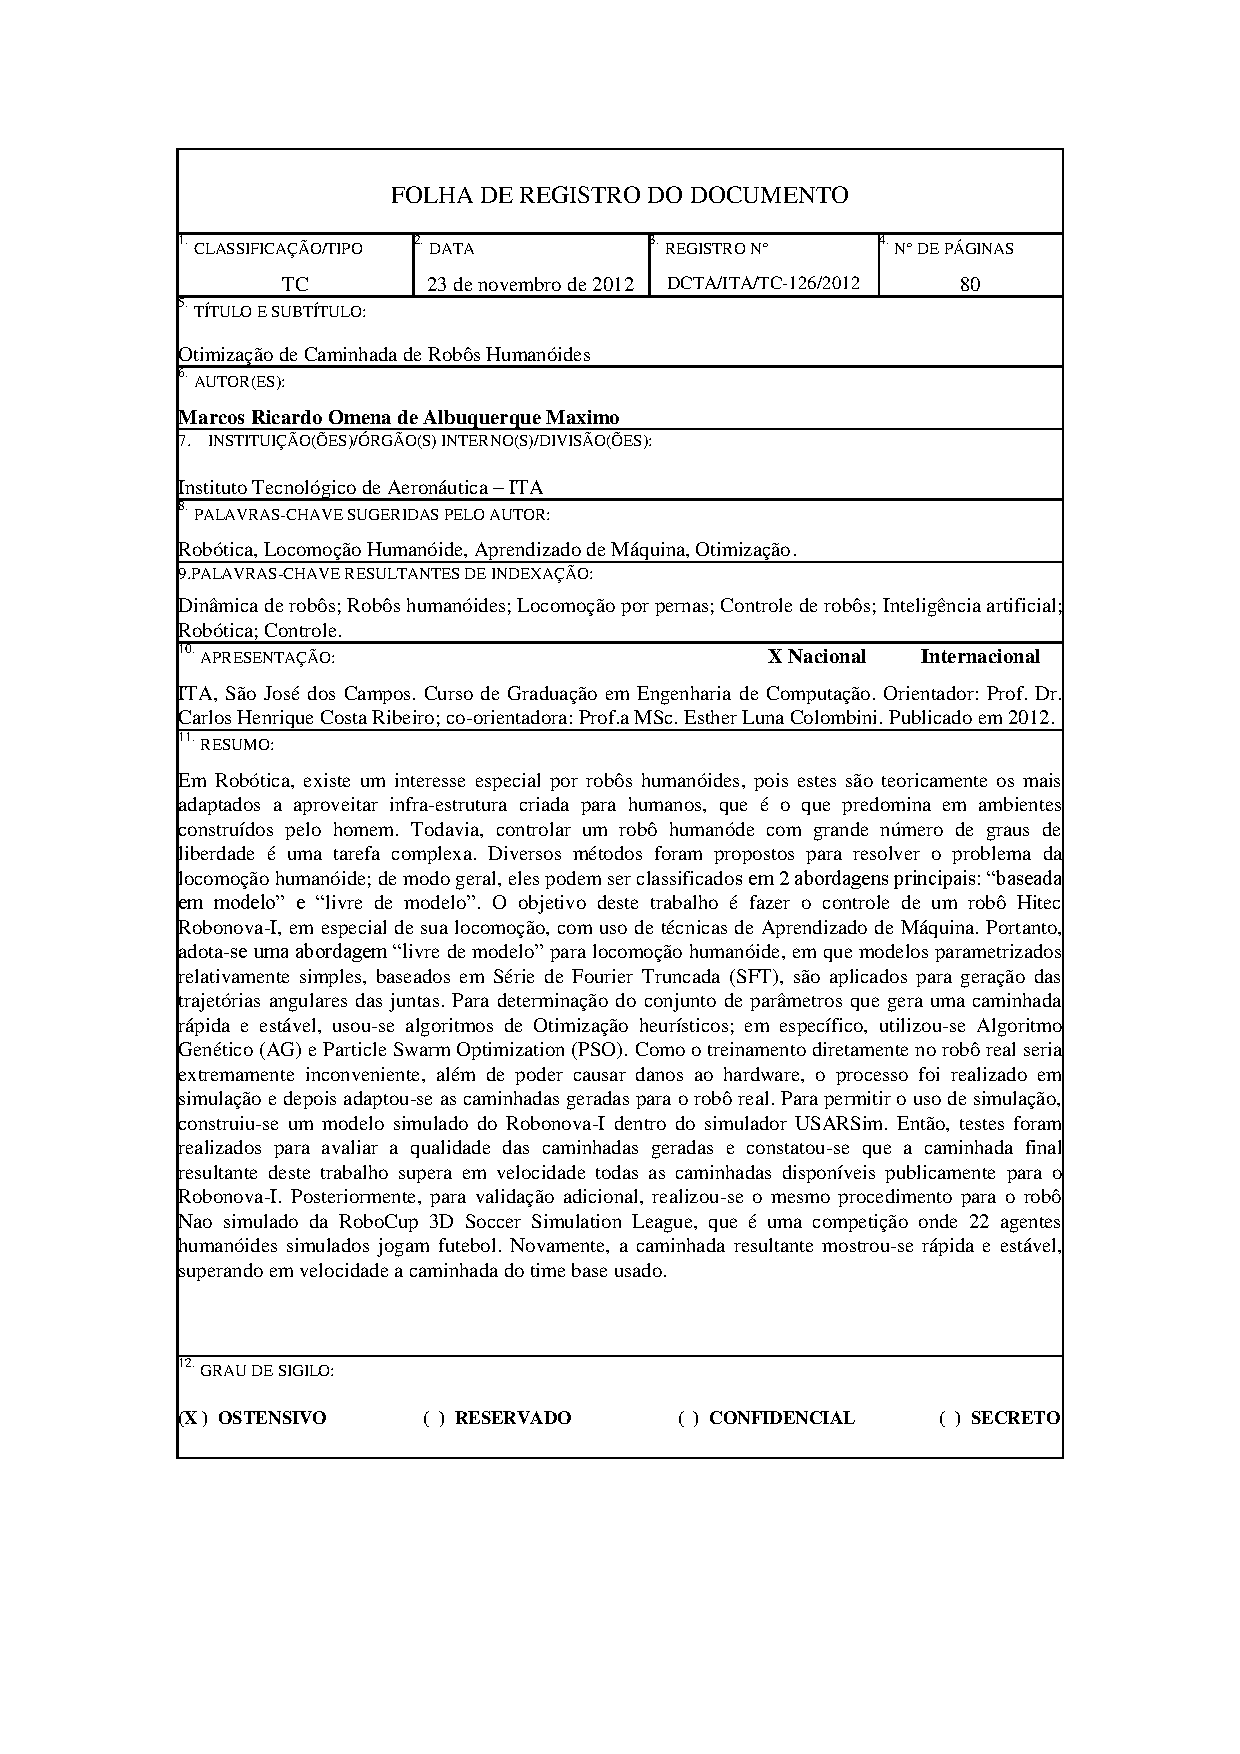
\includepdf{folha_registro_documento.pdf}
\bookmark[level=0, page=75]{Folha de Registro do Documento}

\end{document}